\documentclass[11pt,a4paper]{book} 
\usepackage[pdftex]{geometry}
\usepackage{fancyvrb}
\usepackage[dvips]{graphicx}
\usepackage{framed}
\usepackage{moreverb} % env: comment
\usepackage{amssymb,amsmath}
%\usepackage{alltt} 
%\usepackage{pifont} 
%\usepackage{color} 
%\usepackage{subfigure}
%\usepackage{listings}
%\usepackage{epstopdf}
%\DeclareGraphicsRule{.tif}{png}{.png}{`convert #1 `dirname #1`/`basename #1 .tif`.png}
%\usepackage{draftwatermark} 
%\SetWatermarkLightness{0.9}
%\SetWatermarkFontSize{20cm}
%\SetWatermarkScale{5.0} 

\title{An Introduction to Computer Programming\\
  Using Groovy and Java} % and maybe Java Decaf in the future
\author{Sergio Gutierrez-Santos\\
  Birkbeck, University of London}

\date{\InputIfFileExists{version.txt}
     {v}
     {version unkown}} % "version.txt" not found

\pagestyle{plain}

\begin{document}

%%%%%%%%%%%%%%%%%%%%%%%%%
%      TITLE PAGE       %
%%%%%%%%%%%%%%%%%%%%%%%%%

\maketitle

\thispagestyle{empty}

\vfill 

\begin{figure*}[h!]  % BBK logo
  \centering
  
\includegraphics[height=2cm]{bbk.eps}
\end{figure*}

\vfill

\noindent (Last revision: \today.)

%\vfill 

\newpage

~\vspace{8cm}

\textbf{Important note: } If anything is unclear, or you have any 
sort of problem (e.g.,
downloading or installing Groovy on your computer), please send an
email to Sergio Gutierrez-Santos (\emph{sergut@dcs.bbk.ac.uk}).

\textbf{Acknowledgements: } I am in great debt with 
Keith Mannock for his invaluable help in the initial stages of
preparing this document, and also with Roger Mitton for his C++ notes
(based on work by S.P. Connolly) that influenced its genesis. 
Thanks to all reviewers that have helped to 
find typos, errors, and omisions. Although they are too numerous to
name them all, I could not go without mentioning Alexandra
Poulovassilis for her \emph{beyond the call of duty} efforts clean
these notes free of numerical, syntactical, and typographical
\emph{bugs}. Any errors that you, my dear reader, may still find are
only my own fault. 

\newpage

\tableofcontents

% MAJOR REORGANISATION FOR NEXT YEAR:
% 
% Goals: 
%   - Trevor constraint: PT must see trees before D11 has ended
%   - Corolary to the Trevor constraint: PT should go to Xmas 
%       knowing how to use the Java Collections Library 
%   - Recursion constraint: recursion should be understood before 
%       trees are presented
%   - only solution: FT and PT follow different schedules
%   - In PC++ the difficulty is pointers and recursion; in PiJ the 
%       difficulty is pointers and multi-threading (recursion falls
%       down to level 2 of difficulty)
%
% FT:  
%   D1: refresh
%   D2: Git
%   D3: simple / complex types
%   D4: methods
%   D5: arrays, access levels, reading javadoc, differences groovy/java
%   D6: recursion 1
%   D7: recursion 2
%   D8: pointers, lists
%   D9: static, interfaces, stacks, queues, 
%   D10: trees,
%   D11: testing, introducing annotations
%   D12: TDD, final, more annotations, write javadoc
%   D13: inheritance
%   D14: polymorphism (and the collections library)
%   D15: Exception handling
%   D16: I/O
%   D17: concurrency 1: basics: Thread, Runnable, synchronized
%   D18: concurrency 2: java.concurrent and fork/join
%   D19: concurrency 3: CSP?
%   D20: network 1: RPC
%   D21: network 2: REST
%   D22: work in the lab: only one day... for revision

% PT:  
%   D1: refresh
%   D2: Git
%   D3: simple / complex types
%   D4: methods
%   D5: arrays, access levels, reading javadoc, differences groovy/java
%   D6: recursion all in one day (but it IS a full week)
%   D7: pointers, lists
%   D8: static, interfaces, stacks, queues, 
%   D9: trees (and what are arrays for: main method, varargs)
%   D10: inheritance
%   D11: polymorphism (and the collections library)
%   ------- Xmas ---------
%   D12: testing, introducing annotations
%   D13: TDD, final, more annotations, write javadoc
%   D14: Exception handling
%   D15: I/O
%   D16: concurrency 1: basics
%   D17: concurrency 2: java.concurrent and fork/join
%   D18: concurrency 3: CSP? Just more time for practice?
%   D19: network 1: RPC
%   D20: network 2: REST
%   D21: work in the lab: a full fortnight for revision
%   D22: work in the lab: a full fortnight for revision


% Day 0: what do I want from you?
%   - to be self-sufficient learners
%   - to be creative
%   - to be able to read code
%   - to be able to write code (is this the same as being "creative")

% Day 1: welcome to CS!  (assumption: they read the notes already!)
% \item Basics: variables, types, initialization, comments
% \item Flow control: branches, loops
%    add switch/case and ternary operator
%    leave for loops for lists
%    leave do/while for Java, because there is not in Groovy
% Day 2: 
% \item Source code version control
% and lots of exercises, because there is nothing else to tell...
\chapter{Week 1: Here it all begins\ldots}
\section{Introduction}

%Simple input/output with integers, outputting words and ends of lines, assignment and initialisation}

To get a computer to do something, you have to tell it what you want it
to do.  You give it a series of instructions in the form of a \emph{program}.
You write a program in a \emph{programming language}.
Many programming languages have been devised; well known ones include
Fortran, BASIC, Cobol, Algol, Lisp, Ada, C++, Python, Ruby, Scala, and Java.

The language we will use in this document is named \emph{Groovy}, and
it is \emph{very similar to the Java programming language but with a
simplified syntax} that better fits the purposes of this introduction. 

Programming languages vary a lot, but
an instruction in a typical programming language might contain
some English words (such as \verb!while! or \verb!return!), perhaps a mathematical
expression (such as \verb!x + 2!) and some punctuation marks used in a special way.
The following three lines are in BASIC, Cobol and C++ respectively:
\begin{Verbatim}
      FOR I% = 1 TO 100 STEP 5 DO

      PERFORM RECORD-TRANSACTION UNTIL ALL-DONE = "T"

      if (x > 100) cout << "Big"; else cout << "Small";
\end{Verbatim}

Programs can vary in length from a few lines to thousands of lines.
Here is a complete, short program written in Groovy:

\VerbatimInput[frame=single,label=Example]{src/Example1.groovy}

When you write a program, you have to be very careful to keep to the
syntax of the programming language, i.e. to the grammar rules of the language.  
For example, the above Groovy program would
behave incorrectly if in the 13$^{th}$ line we wrote 

\begin{Verbatim}
	if (max = 0)
\end{Verbatim}

instead of 

\begin{Verbatim}
	if (max == 0)
\end{Verbatim}

or if in the 9$^{th}$ line we put a semi-colon immediately after 

\begin{Verbatim}
      if (s.length() > max)
\end{Verbatim}

The computer would refuse to accept the program if we added dots or semi-colons 
in strange places
or if any of the parentheses (or curly braces) were missing, or if we wrote
\verb!leng! instead of \verb!length()! or even \verb!Length()! instead of \verb!length()!.

% Moved to earlier:
% 
%The language we will use in this document is named \emph{Groovy}, and
%it is \emph{very similar to the Java programming language but with a
%simplified syntax} that better fits the purposes of this introduction. 

\subsection{Input and output}

To get the computer to take some input and to store it
in its memory, we write in Groovy:

\begin{Verbatim}
      str = System.console().readLine()
\end{Verbatim}

\verb!System.console().readLine()! (pronounced \emph{system dot
  console dot read line}) is a phrase which has a special meaning to
the computer. The combination of these instructions
means\footnote{More precisely, it means ``Take the current system
  --- this computer, take its console --- its keyboard and screen,
and read a line of character input from it as entered by the user'' (from the keyboard,
not the screen because the user cannot type a line onto the screen... or
could not before they invented touchscreens!)).} 
``Take some input which is a sequence of characters and put it into the computer's memory.''

\verb!str! by contrast, is a word that I (the programmer) have chosen.
I could have used \verb!characters! or \verb!thingy! or \verb!foodle!
or just \verb!s! or almost any word I wanted. (There are some
restrictions which I will deal with in the next section.)  
% You may occasionally see the semi-colon used in a program and that signals the
% end of this instruction.

Computers can take in all sorts of things as input --- numbers,
letters, words, records and so on --- but, to begin with, we will
write programs that generally handle strings of characters (like
"I", "hi", "My mother has 3 cats", or "This is AWESOME!").
We'll also assume that the computer is taking its input from the
keyboard, i.e., when the program is executed, you key in one or more
words at the keyboard and these are the characters that the computer 
puts into its memory.

You can imagine the memory of the computer as consisting of lots of
little boxes.  Programmers can reserve some of these boxes for
use by their programs and they refer to these boxes by giving
them names.  

\begin{Verbatim}
      str = System.console().readLine()
\end{Verbatim}

means ``Take a string of characters input using the keyboard and
terminated when the user presses RETURN, and
then put this string into the box called \verb!str!.''  When the program runs and
this instruction gets executed, the computer will take the words which
you type at the keyboard (whatever you like) and will put them into
the box which has the name \verb!str.!

Each of these boxes in the computer's memory can hold only one string at a time.  If a box is
holding, say, ``hello'', and you put ``Good bye!'' into it, the
``Good bye!'' replaces the ``hello''.  In computer parlance these
boxes are called \emph{variables} because the content inside the box
can vary; you can put an ``I'' in it to start with and later change it
to a ``you'' and change it again to ``That was a hurricane'' and so on
as often as you want.

In Groovy, you have to tell the computer that you want to use a variable
with a certain name before you use it.  You can't just pitch in using \verb!str!
without telling the computer what \verb!str! is.  Most of the time you also have to
tell the computer what {\em type} of variable this is, i.e., what sort of thing you are going
to put into it. In this case we are going to put strings of characters into \verb!str!. 
Strings of characters, or simply \emph{strings} as they are called in programming, are
known in Groovy as \verb!String!, with capital S.  To tell the computer that we want to use a
variable of type \verb!String! called \verb!str!, we write in our program:

\begin{Verbatim}
      String str
\end{Verbatim}

If we wanted to declare more than one variable, we could use two lines:

\begin{Verbatim}
      String myName
      String yourName
\end{Verbatim}

or we could declare them both on one line, separated by a comma:
\begin{Verbatim}
      String myName, yourName
\end{Verbatim}

Your program can have as many variables as you want.  In Groovy you don't
have to declare all your variables at the start of the program, as is the
case in some other languages.  You can declare them in the middle of a
program, but you mustn't try to use a variable before you've declared it.

If you want the computer to display (on the screen) the contents of one of
its boxes, you use \verb!print! followed by the name
of the box.  For example, we can print the contents of \verb!str! by writing:

\begin{Verbatim}
      print str
\end{Verbatim}

If the contents of the box called \verb!str! happened to be ``Karl'', then when the
computer came to execute the instruction \verb!print str! the word ``Karl'' would appear
on the screen.  

% Arithmetic expressions such as \verb!num + 5! can also appear in a \verb!print!
% line.  For example, if \verb!num! had the value 7, then \verb!print num + 5!
% would output 12.
If we use \verb!println! instead of \verb!print! then an extra line is
printed after the value. 

So we can now write a program in Groovy (not a very exciting program,
but it's a start):

\VerbatimInput[frame=single,label=Example]{src/Example2.groovy}

This program takes some text as input from the keyboard and displays it
back on the screen.

It is customary to lay out programs like this with each instruction on a line 
of its own. The indentation, if there is any, is just for the benefit
of human readers, not for the computer which ingnores any indentations. 

\subsection{Compiling and running a program}

You can learn the rudiments of Groovy from these notes just by doing the
exercises with pencil and paper.  It is not essential to run your programs
on a computer.  However, if you have a computer and are wondering how
you run the programs, you will need to know the following, and, even if you don't have
a computer, it will help if you have some idea of how it's done.

First of all you type your program into the computer using a text
editor. Then, 
before you can run the program, you have to \emph{compile} it.  This means that
you pass it through a piece
of software called a \emph{compiler}.  The compiler checks whether your program
is acceptable according to the syntax of Groovy.  If it isn't, the compiler
issues one or more error messages telling you
what it objects to in your program and where the problem lies.
You try to see what the problem is, correct it and try again.  You keep
doing this until the program compiles successfully.  You now have an
{\em executable} version of your program, i.e., your program has been translated
into the internal machine instructions of the computer and the computer
can run your program.

Now you issue a command and the computer executes
your program. You can issue commands\footnote{In
    a modern operating system, you can click on an icon to execute a
    program. However, this only makes sense for graphical applications
    and not for the simple programs that you will write at first.}
from the command prompt in Windows (you can find the command prompt under 
\emph{Start $\rightarrow$
    Accesories}), or from the terminal in Linux and Mac OS/X.  
If you are lucky, your program does what you expect it 
to do first time.  Often it doesn't.  You look at what your program is
doing, look again at your program and try to see why it is not doing what
you intended.  You correct the program, recompile and run it again.
You might have to do this many times before the program behaves in the way
you wanted.

As I said earlier, you can study this introduction without running your
programs on a computer.  However, it's possible that you have a PC with
a Groovy compiler and will try to run some of the programs given in these
notes. 
If you have a PC but you don't have a Groovy compiler, I attach a few notes telling
you how you can obtain one (see Section~\ref{sec:obta-inst-runn}).


\subsection{Outputting words and ends of lines}

Let's suppose that you manage to compile your program 
and that you then run it.  Your running of the above program
would produce something like this on the screen if you typed in
the word Tom followed by RETURN: 

\begin{Verbatim}
Tom
Tom
\end{Verbatim}

The first line is the result of you keying in the word Tom.  The system ``echoes''
the keystrokes to the screen, in the usual way.  When you hit RETURN, the
computer executes the \verb!str = System.console().readLine()! instruction, 
i.e., it reads the word or words that have been input.  Then it
executes the \verb!println! instruction and the word or words that were
input appear on the screen again.

We can also get the computer to display additional words by putting
them in quotes after the \verb!println!, for example:

\begin{Verbatim}
      println "Hello"
\end{Verbatim}

We can use this to improve the above program:

\VerbatimInput[frame=single,label=Example]{src/Example3.groovy}

An execution, or ``run'', of this program might appear on the screen thus:
\begin{Verbatim}
Please key in a word: Tom
The word was: Tom
\end{Verbatim}

Note the spaces in lines 2 and 4 of the program after \verb!word:! and \verb!was:!.
This is so that what appears on the screen is \verb!word: Tom! and
\verb!was: Tom! rather than \verb!word:Tom! and \verb!was:Tom!.

It's possible to output more than one item with a single \verb!print! instruction.
For example, we could combine the last two lines of the above program into one:

\begin{Verbatim}
println "The word was " + str
\end{Verbatim}

and the output would be exactly the same. The symbol ``+'' does not
represent addition in this context, it represents concatenation i.e. 
writing one string after the other. We will look at addition of numbers in the next section.

Let's suppose that we now added three lines to the end of our program, thus:

\VerbatimInput[frame=single,label=Example]{src/Example4.groovy}

After running this program, the screen would look something like this:
\begin{Verbatim}
Please key in a word: Tom
The word was TomNow please key in another: Jack
And this one was Jack
\end{Verbatim}

which is probably not what we wanted.  If we want a new line after the
the first word is printed, we need to use the \verb!println! instruction we mentioned earlier:

\VerbatimInput[frame=single,label=Example]{src/Example5.groovy}

Now we would get:
\begin{Verbatim}
Please key in a word: Tom
The word was Tom
Now please key in another: Jack
And this one was Jack
\end{Verbatim}


\subsection*{Exercise A}

Now pause and see if you can write:
\begin{enumerate}
\item
a Groovy instruction which would output a blank line.
\item
an instruction which would output

\begin{Verbatim}
Hickory, Dickory, Dock
\end{Verbatim}

\item
a program which reads in two words, one after the other, and then displays them
in reverse order. For example, if the input was 

\begin{Verbatim}
First
Second
\end{Verbatim}

the output should be

\begin{Verbatim}
Second
First
\end{Verbatim}

\end{enumerate}

%To check your answers, click on  \verb!Answers to the exercises!. (TO BE COMPLETED)

\subsection{Assignment and initialisation}

There is another way to get a string into a box apart from using
\verb!System.console().readLine()!.  We can write, for instance:

\begin{Verbatim}
    str = "Some text"
\end{Verbatim}

This has the effect of putting the string ``Some text'' into the
\verb!str! box.  Whatever content was in \verb!str! before is obliterated; the
new text replaces the old one. 

In programming, this is called \emph{assignment}.  We say that the
value ``Some text'' is
assigned to the variable \verb!str!, or that the variable \verb!str! takes the
value ``Some text''.  The ``='' symbol is the assignment operator in Groovy.  We are not
testing whether \verb!str! has the value ``Some text'' or not, nor are we stating that
\verb!str! has the value ``Some text''; we are \emph{giving} the value
``Some text'' to \verb!str!.

% Unneeded. Probably should delete.
%
% If we want, we can have arithmetic expressions on the right-hand side of
% the "=", for example:
% \begin{Verbatim}
% num = count + 10
% \end{Verbatim}
% This instruction means, "Take whatever number is in \verb!count!,
% add 10 to it and put the result into \verb!num!."

An assignment instruction such as this:

\begin{Verbatim}
    str = str + " and some more"
\end{Verbatim}

looks a little strange at first but makes perfectly good sense.
Let's suppose the current value of \verb!str! (the contents of the
box) is ``Some text''.
The instruction says, 'Take the value of \verb!str!
(``Some text''), add `` and some more''  to it (obtaining ``Some text and some
more'') 
and put the result into \verb!str!'.
So the effect is to put ``Some text and some more'' into \verb!str! in
place of the earlier ``Some text''.

The \verb!=! operator is also used to initialise variables.  When the computer
allocates a portion of memory to store one of your variables, it does not
clear it for you; the variable holds whatever value this portion of memory
happened to have the last time it was used.  Its value is said to be
\emph{undefined.}

Using undefined values is a common cause of program
bugs.  
% Suppose a program uses the variable \verb!str! without giving it an
% initial value and suppose that, on the computer the programmer is using,
% the initial value in \verb!num! happens to be zero and that, by happy chance,
% zero is just what the programmer wants it to be.
% The program seems to work fine.  Then the program is compiled and run on
% a different computer.  On this second computer, the initial value of \verb!num!
% does not happen to be zero.  The program, which has worked OK on the first
% computer, does not work on the second one.
%
To prevent yourself from using undefined values, you can give a variable
an initial value when you declare it.  For example, if you wanted \verb!str! to begin
with empty, you should declare it thus:

\begin{Verbatim}
      String str = ""
\end{Verbatim}

This is very like assignment since we are giving a value to \verb!str!. But
this is a special case where \verb!str! did not have any defined value before,
so it is known as \emph{initialisation.}

Finally a word about terminology.  I have used the word ``instruction''
to refer to lines such as \verb!println str! and \verb!str = 5!
It seems a natural word to use since we are giving the computer instructions.
But the correct word is actually ``statement''.  \verb!println str! is
an output statement, and \verb!str = "Hello"! is an assignment statement.
The lines in which we tell the computer about the variables we intend to
use, such as \verb!String str! or \verb!String str = ""! are called
variable \emph{definitions}.  They are also referred to as 
variable \emph{declarations}.  When you learn more about Groovy you will
find that you can have declarations which are not definitions, but the
ones in these introductory notes are both definitions and declarations.

\subsection*{Exercise B}

Now see if you can write a program in Groovy that takes
two words from the keyboard and outputs one after the other on the same line. 
E.g., if you keyed in ``Humpty'' and ``Dumpty'' 
it would reply with ``Humpty Dumpty'' (note the space in between).
A run of the program should look like this:

\begin{Verbatim}
    Please key in a word: Humpty
    And now key in another: Dumpty
    You have typed: Humpty Dumpty
\end{Verbatim}

%To check your answers, click on \verb!Answers to the exercises!. (TO BE COMPLETED)

 	

%%% Local Variables:
%%% TeX-master: "primer"
%%% End:


\input{section2-Variables,integers,strings,comments}
\input{section3-If,else}
\section{Loops and booleans}

How would you write a program to add up a series of numbers?
If you knew that there were, say, four numbers, you might write
this program:

\VerbatimInput[frame=single,label=Example]{src/s3Example.groovy}

But a similar program to add up 100 numbers would be very long.
More seriously, each program would need to be tailor-made for a particular
number of numbers.  It would be better if we could write one program
to handle \emph{any} series of numbers.  We need a \emph{loop.}

One way to create a loop is to use the keyword \texttt{while}.
For example:

\VerbatimInput[frame=single,label=Example]{src/s3Example2.groovy}

It is not essential to indent the lines inside the loop, but it makes the
program easier to read and it is a good habit to get into.


Having initialized the variable \texttt{num} to zero, the program checks
whether the value of \texttt{num} is less than 100.  It is, so it
enters the loop.  Inside the loop, it adds 5 to the value of
\texttt{num} and then outputs this value (so the first thing that
appears on the screen is a \texttt{5}).  Then it goes back to the
  \texttt{while} and checks whether the value of \texttt{num} is less than
100.  The current value of \texttt{num} is 5, which is less than 100,
so it enters the loop again.  It adds 5 to \texttt{num}, so
\texttt{num} takes the value 10, and then outputs this value.  It goes back
to the \texttt{while}, checks whether 10 is less than 100 and enters
the loop again.  It carries on doing this with \texttt{num} getting
larger each time round the loop.  Eventually \texttt{num} has the
value 95. As 95 is still less than 100, it enters the loop again, adds 5 to
\texttt{num} to make it 100 and outputs this number.  Then it goes
back to the \texttt{while} and this time sees that \texttt{num} is not
less than 100.  So it stops looping and goes on to the line after the
end of the loop.  (In the case of this program, there are no more
lines, so it finishes.)  The output of this program is the numbers 5,
10, 15, 20 and so on up to 95, 100.

Note the use of curly braces to mark the start and end of the loop.
Each time round the loop the program does everything inside the curly braces.
When it decides not to execute the loop again, it jumps to the point
beyond the closing brace.

What would happen if the \texttt{while} line of this program was
\texttt{while (num != 99)}?
The value of \texttt{num} would eventually reach 95.  The computer would
decide that 95 was not equal to 99 and would go round the loop again.
It would add 5 to \texttt{num,} making 100.
It would now decide that 100 was not equal to 99 and would go round the
loop again.  Next time \texttt{num} would have the value 105, then 110,
then 115 and so on.  The value of \texttt{num} would never be equal to 99
and the computer would carry on for ever.  This is an example of
an \emph{infinite loop}.

Note that the computer makes the test \emph{before} it enters the loop.
What would happen if the \texttt{while} line of this program was
\texttt{while (num > 0)}?   \texttt{num} begins with the value zero and the computer would first
test whether this value was greater than zero.  Zero is not greater than
zero, so it would not enter the loop.  It would skip straight to the end
of the loop and finish, producing no output.

% It is not essential to indent the lines inside the loop, but it makes the
% program easier to read and it is a good habit to get into.

\subsection*{Exercise A}

Write a program that outputs the squares of all the numbers from 1 to
10, i.e. the output will be the numbers 1, 4, 9, 16 and so on up to 100.

\subsection{Booleans (true/false expressions)}

So far we have just used integer and string variables.  But we can
have variables of other types and, specifically, we can have
\emph{boolean} variables\footnote{The word ``boolean'' was coined in honour of an
Irish mathematician of the nineteenth century called \emph{George Boole}}.  
In Groovy, these are variables of type \texttt{boolean}.
A variable of type \texttt{boolean} does not hold numbers;
it can hold just the values \texttt{true} and \texttt{false}.  We
might declare and initialize a boolean variable thus:

\begin{Verbatim}
    boolean positive = true
\end{Verbatim}

Note that we do not have quote marks around the word \texttt{true}.  
The word \texttt{true}, without quote marks, is not a string; it's the name of a
boolean value.  Contrast it with:

\begin{Verbatim}
    String stringvar = "true"
\end{Verbatim}

\texttt{stringvar} is a String variable which is being initialized
with the four-character string ``\texttt{true}''; we could assign any
other string to \texttt{stringvar}. By contrast, \texttt{positive}
is a boolean variable and we cannot assign strings to it.
It can hold only the values \texttt{true} or \texttt{false}.

You have already met boolean expressions.  They are also called conditional
expressions and they are the sort of expression you have in brackets
after \texttt{if} or \texttt{while}.  When you evaluate a boolean expression,
you get the value \texttt{true} or \texttt{false} as the result.

Consider the kind of integer assignment statement with which you are
now familiar:

\begin{Verbatim}
    num = count + 5
\end{Verbatim}

The expression on the right-hand side, the \texttt{count + 5}, is an
integer expression.  That is, when we evaluate it, we get an integer value
as the result.  And of course an integer value is exactly the right kind of
thing to assign to an integer variable.

Now consider a similar-looking boolean assignment statement:

\begin{Verbatim}
    positive = num >= 0
\end{Verbatim}

The expression on the right-hand side, the \texttt{num >= 0}, is a
boolean expression.  That is, when we evaluate it, we get a boolean value
(true/false) as the result.  And of course a boolean value is exactly the
right kind of thing to assign to a boolean variable.  You can achieve
the same effect by the following more long-winded statement:

\begin{Verbatim}
    if (num >= 0) {
        positive = true
    } else {
        positive = false
    }
\end{Verbatim}

The variable \texttt{positive} now stores a simple fact about the value of
 \texttt{num} at this point in the program.  (The value of  \texttt{num} might
subsequently change, of course, but the value of \texttt{positive} will not
change with it.)  If, later in the program, we wish to test
the value of \texttt{positive}, we need only write

\begin{Verbatim}
    if (positive)
\end{Verbatim}

You can write \texttt{if (positive == true)} if you prefer, but the
\texttt{== true} 
is redundant.  \texttt{positive} itself is either true or false.  
%Once the computer has evaluated \texttt{positive} 
%(established whether it is true or false) there is nothing more to do.  
We can also write

\begin{Verbatim}
    if (!positive)
\end{Verbatim}

(pronounced \emph{if not positive}) that is exactly the same as \texttt{if
  (positive == false)}. If \texttt{positive} is true, then not
\texttt{positive} is false, and vice-versa. 

Boolean variables are often called \emph{flags}.  The idea is that
% , leaving aside subtleties such as half-mast, 
a flag has basically two states
--- either it's flying or it isn't.

So far we have constructed simple boolean expressions using the operators
introduced in the last chapter --- \texttt{(x == y), (s >= t)} and so on ---
now augmented with negation~(\verb+!+).
We can make more complex boolean expressions by joining simple ones
with the operators \emph{and} (\verb!&&!) and \emph{or} (\texttt{||}).  For example,
we can express ``if x is a non-negative odd number'' as
\verb+if (x >= 0 && x \% 2 == 1)+. We can express ``if the name begins
with an A or an E'' as \texttt{if (name.substring(0,1) == "A" ||
  name.substring(0,1) == "E")}.  The rules for evaluating \emph{and}
and \emph{or} are as follows:

\vspace{1em}
\begin{tabular}{|l|lcr||lcr|}
\hline
& left & \verb!&&! & right & left & \verb+||+ & right\\
\hline
\hline
1 & true & \textbf{true} & true&true&\textbf{true}&true\\
2 & true & \textbf{false} & false&true&\textbf{true}&false\\
3 & false & \textbf{false} & true&false&\textbf{true}&true\\
4 & false & \textbf{false} & false&false&\textbf{false}&false\\
\hline
\end{tabular}
\vspace{1em}

Taking line 2 as an example, this says that, given that you have two simple
boolean expressions joined by \emph{and} and that the one on the left is
true while the one on the right is false, the whole thing is false.  If,
however, you had the same two simple expressions joined by \emph{or}, the
whole thing would be true. As you can see, \emph{and} is true if and
only if both sides are true, otherwise it's false; \emph{or} is false
if and only if both sides are false, otherwise it's true.

\subsection*{Exercise B}

Given that \texttt{x} has the value 5, \texttt{y} has the value 20,
and \texttt{s} has the value ``\texttt{Birkbeck}'', decide whether these
expressions are true or false:

\begin{Verbatim}
(x == 5 and y == 10)
(x < 0 or y > 15)
(y % x == 0 and s.length() == 8)
(s.substring(1,3) == "Bir" or x / y > 0)
\end{Verbatim}

\subsection{Back to loops}

Returning to the problem of adding up a series of numbers, have a
look at this program:

\VerbatimInput[frame=single,label=Example]{src/s3Example3.groovy}

If we want to input a series of numbers, how will the program know
when we have put them all in?  That is the tricky part, which accounts
for the added complexity of this program.

The \texttt{boolean} variable
\texttt{finished} is being used to help us detect when there are no more
numbers. It is initialized to \texttt{false}.  When the computer detects
that the last number (``0'') is introduced, it will be set to \texttt{true}.
When \texttt{finished} is true, it means that we have finished reading in
the input. The \texttt{while} loop begins by testing whether \texttt{finished}
is true or not.  If \texttt{finished} is not true, there is some more input
to read and we enter the loop. If \texttt{finished} is true, there are
no more numbers to input and we skip to the end of the loop.

The variable \texttt{total} is initialized to zero.
Each time round the loop, the computer reads a new value into \texttt{num}
and adds it to \texttt{total}. So \texttt{total} holds the total of all
the values input so far.

Actually the program only adds  \texttt{num} to \texttt{total} if a (non-zero) 
number has been entered. 
% The user will signal that there are no more numbers by keying in a special
% character.  (On Unix this is a Control-D; on PCs it is usually a Control-Z.
% If this is gobbledygook to you, just imagine that the user strikes a special
% key on the keyboard.)  
If the user enters something other than an integer 
--- perhaps a letter or a punctuation mark --- 
then the parsing of the input will fail 
and the program will stop, giving an error message.
% If the program is expecting an integer
% and instead receives something like ``abc'' or ``W'' or ``**!'', the input will fail.
% We can test whether the input has finished with the line \texttt{if (sc.hasNext())}.
% If this is false, then there is no more input available and we set \texttt{finished} to \texttt{true}
% in order to terminate the loop.

A real-life program ought not to respond to a user error by aborting
with a terse error message, though regrettably many of them do.
However, dealing with this problem properly would make this little program
more complicated than I want it to be at this stage.

\textbf{You have to take some care in deciding whether a line should go in the
loop or outside it}.  This program, for example, is only slightly different
from the one above but it will perform differently:

\VerbatimInput[frame=single,label=Example]{src/s3Example4.groovy}

It resets \texttt{total} to zero \emph{each time round the loop.}  So
\texttt{total} gets set to zero,
has a value added to it, then gets set to zero, has another value added to
it, then gets set to zero again, and so on.  When the program finishes,
\texttt{total} does not hold the total of all the numbers, just the value
zero.

Here is another variation:

\VerbatimInput[frame=single,label=Example]{src/s3Example5.groovy}

This one has the \texttt{print} line inside the loop, so it outputs the value
of \texttt{total} each time round the loop.  If you keyed in the numbers
4, 5, 6, 7 and 8, then, instead of just getting the total (30) as the output,
you would get 4, 9, 15, 22 and then 30.

\subsection*{Exercise C}

Write a program that reads a series of numbers, ending with 0, and then tells you how
many numbers you have keyed in (other than the last 0).  For example, if you keyed in the
numbers~5, -10, 50, 22, -945, 12, 0 it would output ``You have entered 6
numbers.''.


% \subsection{System libraries}

% The purpose of libraries is to provide the programmer with extensions
% to the language which can be pulled in, as and when needed. 
% Some libraries, known as the standard libraries, are provided with every
% Groovy implementation.  Other libraries can be created for special purposes.

% One team of programmers might produce a library of routines for another
% team of programmers to use.  When teams of programmers divide up the
% work on a large program in this way, it is all too easy
% for programmers in team A to choose a name for some item in their library
% and for programmers in team B to choose
% the same name for some quite unrelated item elsewhere in the program.
% This can be a serious nuisance.  To help contain the problem, Groovy
% provides \emph{packages}.  Team A declares one namespace and team B
% declares another.  Now it doesn't matter if they accidentally choose the
% same name.  Team B can still use names from A's package, but they have to
% tell the compiler specifically which names they are going to use.




%%% Local Variables:
%%% mode: latex
%%% TeX-master: "main"
%%% End:



\section{More on branches}
\label{sec:more-branches-loops}

You can write a lot of different programs with the little
\texttt{if\ldots else} and \texttt{while} constructs you have already
learned and practiced, for executing different branches in your
program and for running loops. There are, however, other constructs
that you can use to make your programs clearer. In this section we
will learn about the \texttt{do\ldots while} loops, the
\texttt{switch\ldots case} multiple branching feature, and the
so-called ternary operator. In later chapters, we will also see how to
use the very useful \texttt{for} and \emph{for each} loops. 

\subsection{Multiple branching}
\label{sec:multiple-branching}

Look at the following code, that loosely resembles an automatic
phone-answering program:

\VerbatimInput[frame=single,label=Example]{src/s5E1.groovy}

Such a long list of \texttt{if} branches can be a bit confusing for
future readers. When there are many options, and especially if the
options are finite and known in advance, it is better to make the
multiple branching clearer by using a \texttt{switch\ldots case}
construct, as in the following example:

\VerbatimInput[frame=single,label=Example]{src/s5E2.groovy}

As you can see, the multiple branches are introduced by the keyword
\texttt{switch} followed by some parameter, \emph{choice} in this
case. Then several possible cases follow, each of them starting by a
semicolon. The whole list of cases is inside two curly brackets, but
the code of each case does not need curly brackets. 

There are two important things to note in this program. First, there
is a keyword \texttt{break} at the end of each case. This is very
important. Without it, Groovy will finish the execution of one case
and continue with the next one. Second, there is a default case that
is executed if none of the other cases matches \emph{choice}. This is
also important: always write a default case for your
\texttt{switch\ldots case} structures. They are good for detecting
errors in your program. 

\subsubsection*{Exercise A}

Write a program like the one in the last example, but add a little
code for each case (some \texttt{println} statements will do) and
remove the \texttt{break} keywords. Execute the program and see what
happens. 

\subsubsection*{Exercise B}

Write a program similar to the one in the former example, but a bit
better. Make the computer ask for an option and then execute the
corresponding code in a \texttt{switch\ldots case} structure. If the
user introduces an invalid option (e.g. 9 in the example above), make
the computer say ``That is not a valid option, please try again'', and
ask again until the user enters a valid numbers. Hint: You will need
to use a loop and change the default case. 

\subsubsection*{Exercise C}

Write a program that uses Strings instead of integers for the
\texttt{switch}. What happens?

\subsubsection{What types can go inside a \texttt{switch}}
\label{sec:what-types-can}

If you have tried all the exercises above, you have noticed that
Groovy complains when you try to use Strings inside a
\texttt{switch\ldots case}. The bad news is that we cannot use any
type of data, but only things like integers, characters (also known as
\emph{chars} for brevity), and enumerated types (also known as
\emph{enums}, we will come to them in a second). The good news is that
this is usually enough.

Characters can be used alone in any Groovy program, can be printed on
the screen, and can also be
combined to form our well-known Strings, as in the following code: 

\VerbatimInput[frame=single,label=Example]{src/s5E3.groovy}

Notice that single quotes are used for characters and double quotes
are used for Strings: \'c\' is the character \emph{c}, but ``c'' is a
String with only the character \emph{c} in it. 

\subsubsection{What are \emph{enums}}
\label{sec:what-types-enum}

Enumerated types (usually called \emph{enums}) 
are just lists of \emph{tags} that can be useful to
make your program more legible. They can be used to specify constants
that have some special meaning. Defining an \emph{enum} in Groovy is
really easy: 

\begin{verbatim}
    enum Day {
      MONDAY,
      TUESDAY,
      WEDNESDAY,
      THURSDAY,
      FRIDAY,
      SATURDAY,
      SUNDAY,
    }
\end{verbatim}

Once an \emph{enum} is defined, it can be used to declare new variables in
the same way that we define them as String or int. 

\begin{verbatim}
    Day dayOfWeek;
    dayOfWeek = Day.MONDAY;
\end{verbatim}

Now, an enum can be used in \texttt{switch} (or \texttt{if})
statements. Compare the clarity of this code:

\begin{verbatim}
    switch (day) {
      case 1: 
        // do something here for this day
        break;
      case 3: 
        // do something here for this day
        break;
      ...
    }
\end{verbatim}

and this code:

\begin{verbatim}
    switch (day) {
      case Day.MONDAY: 
        // do something here for this day
        break;
      case Day.WEDNESDAY: 
        // do something here for this day
        break;
      ...
    }
\end{verbatim}

In the second case, it is clear what each case is for. In the first
piece of code, you need to guess: look at the code for each case, look
at the surrounding code\ldots it is harder. Programming is already a
hard (and fun) activity. It is wise not to make it harder than it is;
it does not make it any funnier. 

There is a general lesson to learn here. What you see in the code
above is an example of \emph{magic numbers}: numbers that appear in
your code and have an effect, but is difficult to understand what
their effect is or why they are what they are (i.e. why a~1~and not
a~5?). \textbf{Magic numbers make code harder to read and
  understand. Never use magic numbers in your code.}

\subsection{The ternary operator}
\label{sec:ternary-operator}

There is another form of writing a branch. It is not commonly used,
but you should know it exists. It is the so-called \emph{ternary
  operator}. 

Most operators in Groovy are either \emph{unary} (they take one
argument, like logical NOT~``!'') or \emph{binary} (they take two
arguments, like logical AND~``\&\&'' or addition~``+''). There is only
one ternary operator, with three arguments, that is really another
fancy way of writing an \texttt{if\ldots else} clause. We will
illustrate how it works with a simple example:

\begin{verbatim}
    print "Enter a number: "
    int i = Integer.parseInt(System.console().readLine())
    String s = (i > 5)? "Greater than 5" : "Not greater than 5"
    println s
\end{verbatim}

This code behaves exactly in the same as the following code:

\begin{verbatim}
    print "Enter a number: "
    int i = Integer.parseInt(System.console().readLine())
    String s;
    if (i > 5) {
      s = "Greater than 5"
    } else {
      s = "Not greater than 5"
    }
    println s
\end{verbatim}

As you see, the ternary operator takes three arguments: a boolean
expression and two values. If the boolean expression is true, then the
second argument is returned; if it is false, it returns the third
argument. 

In some cases the ternary operator can make your code clearer, but
these cases are few and far between. In general, it is easier to write
\emph{bona fide} \texttt{if} statements. However, you may find the
ternary operator in code written by others, and it is thus important
to understand how it works. 

\subsubsection*{Exercise D}

Write a program that reads a series of numbers from the user, until the
user enters the String ``END''. The program
should then print how many numbers were positive, negative, or
zero. Write the program using (a) \texttt{if\ldots else} clauses first 
and then using (b) the ternary operator. 
Is there any difference? In which case it is
easier to write the program? In which case does it look clearer to you?

\subsection{It's a kind of magic}
\label{sec:its-kind-magic}

The ternary operator is not the only strange way of making your code
shorter. Incremental operations are so common that combinations of
symbols are used ---in a slightly cryptic way--- to make those code
lines shorter.

Incremental lines are lines in which the value of a variable
(typically \verb+int+) is incremented by some explicit value or the
value of another variable, for example: 

\begin{verbatim}
    time = time + lap;
    depth = depth + drillDepth;
\end{verbatim}

This can be written in a shorter way like: 

\begin{verbatim}
    time += lap;
    depth += drillDepth;
\end{verbatim}

The same principle can be applied to most binary operators, including
subtraction, multiplication, division, and string concatenation; so: 

\begin{verbatim}
    record = record - difference; 
    result = result * 2;
    name = name + newTitle;
\end{verbatim}

become: 

\begin{verbatim}
    record -= difference; 
    result *= 2;
    name += newTitle;
\end{verbatim}

A particular example is the increment of integer variable by one or
minus, used for all sorts of counters:

\begin{verbatim}
    time = time + 1;
    count = count + 1;
    i = i + 1;
    timesLeft = timesLeft - 1;
\end{verbatim}

which are most often written much more shortly as: 

\begin{verbatim}
    time++;
    ++count;
    i++;
    timesLeft--;
\end{verbatim}

There is a small difference between the line \verb-i++- and the line
\verb-++i-. The former evaluates the statement and then increases the
value of \verb+i+ while the later increases the value of \verb+i+ and
then evaluates the statement. This a subtle difference that you should
now worry about and should actually avoid in modern code. In other
words: never write any code that would behave differently if you
changes all instances of \verb-i++- for \verb-++i-. This is very easy
to do by just following the following rule: 

\begin{center}
  \vspace{1em}
  \textbf{\large If you use i++ or similar, make sure it is the only
  thing you write in that statement; do not combine it with anything else. }
  \vspace{1em}
\end{center}




%%% Local Variables:
%%% mode: latex
%%% TeX-master: "main"
%%% End:



% Week 2: getting up to speed, but not quite
% Day 3: 
% \item Simple and complex data types: primitive types (introducing
%    float and double), strings, 
%    classes without methods... use of "new" and "null"
% \item Let them create structs and modify them
%   - CHANGE: instead of levels of access, basics of regular
%       expressions!  -> and String.split()
%
% Day 4:
% \item For loops? -> already covered... where should this be in the
%       book? 
% \item Maybe?? They have seen classes -> levels of access
%       No, leave for D5
% \item Functions/Procedures/Methods, parameters (look at week 4
%   in C++) 
%   \item talk about side effects -> procedures
%   \item including a bit on already know methods like substring()
%       Update: Not needed, except as an example
%   \item scope: variables inside the methods are copied... but 
%     beware of what happens with complex types! Many exercises
%     about this!
%       Update: 
% \item Optional? Basics of regular expressions -> Update: no! Too much.
%     Maybe better access levels first, regular expressions later
%     Definitely!
%     Update: they are having trouble with moving pointers and copying
%     pointers around. Better leave regular expressions for the
%     future.
\chapter{Week 2: Moving on\ldots}

\section{Simple data types}
\label{sec:simple-data-types}

Programs have lots of data, they are basically
ways of getting data, transforming data, and giving data back to the
world. 
%
A data type, as we have already seen, tell you which kinds of data you
have in your program. 

Simple data types can be thought as boxes in the computer's
memory. Every time you declare a variable in your program, you can
think\footnote{This is only a metaphore and is not supposed to be an
  accurate description of how memory is managed on a modern
  computer. Explaining how things like the registers, the stack, and
  the heap work, the differences between actual machines and virtual
  machines, etc; are out of the scope of this document.} of the
computer as creating a little box in its memory to store your
variable. That box has two tags on it: one of them holds the name of
the variable and the other holds the type
(Figure~\ref{fig:github}). In the same way, you can think of
assignment as putting a value inside that box. 

\begin{figure}
  \centering
  \includegraphics{gfx/no_figure}
  \caption{Declaring a variable in Groovy can be seen as creating a
    box. The box has a tag for the name and another for the type.}
  \label{fig:var1}
\end{figure}

\begin{figure}
  \centering
  \includegraphics{gfx/no_figure}
  \caption{Assigning a value to a variable can be seen as putting a
    value in the box.}
  \label{fig:var1}
\end{figure}

\subsection{Strong typing and weak typing}
\label{sec:strong-typing-weak}

You have already seen that Groovy, as most languages, puts some
restrictions to what you can use as a ``name'' tag for your boxes. You
know that they have to start with a letter: ``count'' is a valid name
but ``/me'' or ``5thNumber'' are not. You also know that some words
cannot be used by the programmer for variables names because it would
be confusing, e.g. ``while'', ``if'', ``System'', or ``println''.

Many programming languages also place one restriction on the ``type''
tag: once you decide the type of a variable, you cannot change
it. This is like people having static opinions that they do not want
to change. This type of languages are called \emph{statically typed
  languages} and, contrary to people with fixed ideas, they are
not necessarily bad or obnoxious. Java is an example of
statically typed language. 

Some programming languages allow you to change the type of your
variables as you go along, so you can have a variable that sometimes
is an int and later in time is a boolean or a String. These languages
are called \emph{dynamically typed languages}. They have pros and cons
compared to their statically typed counterparts. Groovy is an example
of a dynamically typed language. The following code excerpt is valid
in Groovy but not in Java. In Java a variable cannot be a String, and
then a boolean, and then a String again. Note that \emph{true} is a
boolean while \emph{``true''} (in quotes) is a String. 

\begin{verbatim}
    String str = "This is a string";
    str = true;   // This is different to: str = "true"
    if (str) {
      str = "This is a different string";
    }
\end{verbatim}

\subsection{Most common simple types}
\label{sec:most-common-simple}

\subsubsection{Integer numbers}
\label{sec:integers}

\subsubsection{Floating-point (decimal/rational) numbers}
\label{sec:float-point-decim}

\subsubsection{Boolean (binary) values}
\label{sec:bool-binary-valu}

\subsubsection{Characters}
\label{sec:characters}



% ...

You may have noticed that we have not mentioned String yet. This is
because String is a complex type. 

\section{Complex types}
\label{sec:complex-types}




%%% Local Variables:
%%% mode: latex
%%% TeX-master: "main"
%%% End:


\section{Methods}
\label{sec:methods}

We have briefly introduced the concept of
\emph{methods}. In the last section we have seen that they have an
\emph{identifier}, like variables, and that they have (round)
brackets. Sometimes we can put variables or values inside the brackets
like with methods \verb+charAt()+ or \verb+substring()+ of class
String. 

Let's look at methods in a bit more detail now, because they are very
important. 

\subsection{Why are methods important?}

Imagine that you are writing a program in which you need to make some
checks on user input. For example, your program needs the user to
introduce several logins/usernames and the program must make sure that
they do not contain spaces and they are all lower case letters. You
could have some code like:

\begin{verbatim}
    String login = System.console().readLine();
    boolean loginIsValid = true;
    for (int i = 0; i < login.length(); i++) {
        char c = login.charAt(i);
        if (!Character.isLetter(c) || !Character.isLowerCase(c)) {
            loginIsValid = false;
        }
    }
\end{verbatim}

As you can see, the loop goes through the whole length of the string
\emph{login} checking that each and every character is a letter in
lower case. If that is not the case, the boolean flag
\emph{loginIsValid} is set to \verb+false+ so the program knows that a
new login must be asked from the user.

Now you can think of this code being necessary at different parts of
your program. This can be useful (1) when you are adding new users to the
program, (2) when you are changing the username of a user, and (3) when
you want to remove a user from the system, to name but a few. If you
have to write the same code for every single place that you need it,
you have too problems.

First of all, it is \textbf{boring}. You have to type it several
times. Even if you copy--and--paste, you have to find the file where
it is (normal programming projects have tens of hundreds of source
code files, and sometimes they are quite long). Programmers like to
make computers work for them and not the other way around.

Second, but most important, if you find an error (a so-called
\emph{bug}) in those lines of code, you only need to fix in one
place. If you have to fix it in several places, sooner or later you
will forget to do it because you are human. That means that your
program will still be \emph{buggy} even if you are sure you have fixed
it, which is the worse thing than can happen to you. There is a very
important rule in programming that is usually referred to as the DIE
principle: 

\begin{center}
\vspace{1cm}
\textbf{\large DIE: Duplication Is Evil}
\vspace{1cm}
\end{center}

Duplication of information will result in problems sooner or later, so
we must avoid it. This is what methods are for. They allow the
programmer to put code in just one place that can be used from
anywhere else in the program. This means that, for example, if you
need to fix a bug, you fix it in only one place; and if you need to
improve the code to add a new feature, or to make it faster, or for
any other reason, you only need to change it in one place. That way
you are sure that you fix things once and forever. 

Besides, separating code in methods also makes your code
clearer. Compare the easiness of reading the code above with the
following statement: 

\begin{verbatim}
    String login = System.console().readLine();
    boolean loginIsValid = containsOnlyLowerCaseLetters(login)
\end{verbatim}

What is under the hood of that \verb+containsOnlyLowerCaseLetters()+
method? Let's see it. 

\subsection{Defining a method}

A method is defined by its name, its return type, and the parameters
inside the brackets. We will look at parameters in the next section.

A method's name must be an identifier
like those used for variables: starting with a letter and consisting
of letters, digits, and underscores (``\_''). Actually, underscores
are rarely used when you are programming in Java. Methods
usually have names consisting of a single word
(e.g.~\verb+length()+) or several words in so-called \emph{camel case}
starting with a verb (e.g.~\verb+isLetter()+
or~\verb+containsOnlyLowerCaseLetters()+). Note that variables usually
have identifiers that are a noun or an adjective, not a verb.

The return type of a method is a data type, simple or complex, that is
returned by the method when it finishes. When a method finishes, it
must return a value of the appropriate data type by using the keyword
\verb+return+. For example, the method we defined above could look
like the following code:

\begin{verbatim}
    boolean containsOnlyLowerCaseLetters(String login) {
        boolean result = true;
        for (int i = 0; i < login.length(); i++) {
            char c = login.charAt(i);
            if (!Character.isLetter(c) || !Character.isLowerCase(c)) {
                loginIsValid = false;
            }
        }
        return result;
    }
\end{verbatim}

Note that the code is the same that we wrote before. The difference is
we only need to write it once and can use it from anywhere else in the
program just by using its name. We are avoiding duplication of
code. That is good. 

You will notice that this method has a return type ``boolean'', so we
must create a boolean variable and return it at the end. The return
statement is the last statement that is executed inside any method:
once you return the value, there is nothing else to do. This means
that we can make our method a bit more efficient by returning early: 

\begin{verbatim}
    boolean containsOnlyLowerCaseLetters(String login) {
        for (int i = 0; i < login.length(); i++) {
            char c = login.charAt(i);
            if (!Character.isLetter(c) || !Character.isLowerCase(c)) {
                return false;
            }
        }
        return true;
    }
\end{verbatim}

Instead of traversing the whole string, we return \verb+false+ as soon
as we find a character in the login that is not a letter or is not
in lower case. If we arrive at the end of the login, that means that
all characters are fine and we can return \verb+true+. Note that the
loop is automatically terminated when the method is finished,
i.e.~when the return value is given back. It does not matter if the
loop has run to the end or not, or whether there is more code after
the \verb+return+ statement. 

This is important.
It means that you can only return from a method once. Even if you have
several \verb+return+ statements, your program will only execute the
first one it encounters. This does not mean that you can only return
one piece of data from any method; remember that the return value can
be any simple or complex data (like String or Person). By returning a
complex type, you can return as much information as you want. 

You have noticed that there is something inside the round brackets, a
String called \emph{login}, that is used inside the method. The
variables inside the round brackets are called the \emph{parameters} of the
method. 

\subsection{Positional parameters}
\label{sec:pospar}

You can think of methods as small mini-programs: they get some input,
they produce some output. The output is the return value, the input
are the so-called \emph{positional parameters}. 

Positional parameters are declared in the same way as any other
variable. The programmer must specify the type and give it a name, an
identifier. Parameters can have any type, simple or complex, and
separated by commas. If a method does not return any value, the
keyword \verb+void+ is used as return data type. 

In the body of the method (what comes inside the curly
brackets) parameters are used the same as variables declared and
initialised inside the method. Parameters are initialised when the
method is called (see below). 

Some methods do not have any parameters. If that is the case, the
method is defined and called with an empty list of parameters,
i.e.~empty brackets. The method \verb+length()+ is an example of a
method without parameters. 

\emph{Positional} parameters get their name because they come in some
order and they must be called \emph{in the same order}. Let's see how
this is done. 

\subsection{Calling (i.e.~using) methods}
\label{sec:using}

You have already seen how to use some methods, like methods
\verb+length()+ or \verb+substring(int,int)+ of strings\footnote{As
  you can see, now that you know that methods have parameters I will
  start referring to them in a proper way, specifying the type of
  their parameters.}. They are methods of a
class, so you access them with the name of the variable and a dot: 

\begin{verbatim}
    int familyName = fullName.substring(6,12);
\end{verbatim}

This is called \emph{calling}, \emph{executing}, or \emph{running} the
method (the first term is more common). 
You call a method by using its name and specifying the value of its
parameters. 
It is important to call a
method with the right parameters in the right order. For example, if
you have a method like \verb+repeat(String s, int times)+ you 
cannot call it like \verb+repeat(3, "Some text")+ because you will get
an error. Note are well that you do not need to say the type of the
parameters: the computer already know because they are specified in
the method's definition. 

\subsection{Scope}

In a way, you can see the execution of a method as the execution of a
small program in which some of the variables (the parameters) are
initialised in advance (with the values given by the caller). 

A method has access to variables outside of it, but its own variables
are hidden from the rest of the world. They cannot be read or modified
from outside the method. In technical terms, the \emph{scope} of
variables inside the method is the method itself. 

Actually, scope is not just a property of methods. In Java, scope is
roughly defined by any pair of curly brackets, so loops and classes
have scope too. That is why you must use the name of a class to access
variables inside the class, because otherwise they are restricted to
be used \emph{in their scope}. 

But what happens with the method's parameters? They are like variables
for the method but they also come from outside the method, don't they?
Good question. 

When you call a method, the variables used to initialise the
parameters are \emph{copied}, and the copies are used instead of the
original variables. This means that any change to the method's
parameters is forgotten as soon as the method returns. You can check
for yourself by running the following code: 

\begin{verbatim}
    void add1000(int number) {
        println "Starting method, parameter is " + number;
        number = number + 500;
        println "In the middle of method, parameter is " + number;
        number = number + 500;
        println "Ending method, parameter is " + number;
    }
    int myNumber = 0;
    println "Starting program, my number is " + myNumber;
    add1000(myNumber);
    println "After the method is used, my number is " + myNumber;
\end{verbatim}

The output is: 

\begin{verbatim}
    Starting program, my number is 0
    Starting method, parameter is 0
    In the middle of method, parameter is 500
    Ending method, parameter is 1000
    After the method is used, my number is 0
\end{verbatim}

You can see that the value of \emph{myNumber} never changes. The
method made a copy of \emph{myNumber}, used it (under the name
\emph{number}) inside the method, and then forgot it as soon as the
\verb+return+ statement was reached. 

\subsubsection*{Void methods}
\label{void}

Note also that the method does not return anything (i.e.~return type
is \verb+void+). When this is the case, there is no need to have a
return statement because there is nothing to return, and the method
ends after the final statement is reached or when the first \verb+return+
statement is found (with no value). 


\subsubsection{Beware of parameters of complex types!}
\label{beware}



% scope and duplication of variables
  % beware of complex types!

% methods in classes

% side effects

% Flow of execution

% access levels


%%% Local Variables:
%%% mode: latex
%%% TeX-master: "main"
%%% End:


% Day 5: From Groovy to Java (only 1 day)
% \item More on classes and objects: initialization and
% constructors (what "new" really does), 
%      - PLUS access levels
%        \item Information hiding
%        - Levels of access in Java
%          - All variables private unless good reason
%          - Methods public or private depending on target public
%
%   NOTE: no main method, no real java today: continue working from Groovy
%   script ---> BUT YOU NEED TO COMPILE THE CLASSES with javac!
%      - explain some basic classes and their main methods, like String
%      (equals, substring(*), length (*), intValue, doubleValue),
%      Integer (parseInt), Math, System
%      - introduce them to (reading) JavaDocs: constructors, methods, deprecated
%      - make them do exercises with their own classes: create them, 
%        make objects, use them
%   - casting of simple types
%   - chars with 'c', Strings with "c"
%   - arrays and multi-dimensional arrays, 
%   exercise: enter a matrix and say if it is simmetrical
%   exercise: hundir la flota
%             y luego hundir la flota pintando en la pantalla
%   - Update: sometimes Groovy cannot use Java classes. Investigate. TODO
% 
% ASSIGNMENT: class Library (and class Book, and class User): enter
%    new books, enter new Users, take books (max 3 per user), return
%    books; only three classes, and only public what needs to be
%    public (check by reflection)
\chapter{Week 3: From Groovy to Java}

\section{More on clases}
\label{sec:more-clases}

There are two important aspects of classes that we have to learn
about. I am talking about constructor methods and levels of access. 

\subsection{Constructor methods}
\label{sec:constructor-methods}

When classes have been used in the preceding sections, they were used
in two steps: first the memory was reserved for them using \verb+new+
and then their fields were initialised. 

\begin{verbatim}
    Point corner = new Point();
    corner.x = 4;
    corner.y = 0;
\end{verbatim}

This is not too cumbersome unless you have a class that has much more
than two fields that need initialising. For example, if you wanted to
create a \verb+Person+ with first name, family name, gender, age, job,
nationality, etc, you would need a lot of code every time you created
a new \verb+Person+. 

\begin{verbatim}
    Person john = new Person();
    john.firstName = "John";
    john.familyName = "Smith";
    john.gender = Gender.MAN; // This is an enumerated type
    john.age = 30;
    // the rest of the parameters would come here...
    // ...
    Person mary = new Person();
    mary.firstName = "Mary";
    mary.familyName = "Jordan";
    mary.gender = Gender.WOMAN;
    mary.age = 33;
    // the rest of the parameters would come here...
    // ...
\end{verbatim}

We have written a lot of code and we have just created two
objects. This is really boring. On top of that, it looks like we are
repeating code over and over again by having to initialise all fields
manually. There is a better way of doing this. 

Every class (or complex type) can have one or more \emph{constructor
  methods}. A constructor method is a special type of method that is
used to initialise an object of a class when it is first created, and
it is executed every time a new method is created using \verb+new+. In
other words, the constructor method is a way of telling Java to use
\verb+new+ to allocate the memory \emph{and} initialise the object
at the same time. Simpler. Clearer. 

A constructor method looks like a method without a return type (not
even \verb+void+). Have a look at this example:

\begin{verbatim}
class Point {
    double x;
    double y;
    
    Point(double x, double y) {
        this.x = x;
        this.y = y;
    }
    
    double moveTo(Point remote) {
        this.x = remote.x;
        this.y = remote.y;
    }
    
    // more methods here...
}
Point point = new Point(1,1);
println "The point is now at " + point.x + "," + point.y
Point remotePoint = new Point(10,20);
point.moveTo(remotePoint);
println "The point is now at " + point.x + "," + point.y
\end{verbatim}

No need to initialise the points after creating them. The constructor
method does it for both of them. 
If a class has more than one constructor method, Java chooses the
right one according to the positional parameters. For example, we
could create a class Rectangle that has one or two parameters, and
then create different instances (i.e.~objects) of it: 

\begin{verbatim}
class Rectangle {
    int length;
    int width;
    Rectangle(int length, int width) {
        this.length = length;
        this.width  = width;
    }
    // This method creates a square, all sides equal
    Rectangle(int length) {
        this.length = length;
        this.width  = length;
    }
}
Rectangle dominoRectangle = new Rectangle(1,2);
Rectangle pitagoreanRectangle = new Rectangle(3,4);
Rectangle goldenRectangle = new Rectangle(1618,1000);
Rectangle square = new Rectangle(5); 
\end{verbatim}

Every class has 
\textbf{at least one} constructor method. 
If it is not explicit ---as it has been
the case with all classes in the previous sections---, Java 
implicitly adds an empty
constructor: a constructor method with no parameters that does not
initialise any field. 


\subsection{Levels of access (public, private) and information hiding}
\label{sec:levels-access-inform}

A real programming project can have thousands of classes, and millions
of live objects in memory at any given time (remember that we create a
new object every time we use \verb+new+). Keeping track of all the
interactions of these objects becomes very complex very quickly. That
is why programmers make an effort to keep 
the complexity as low as possible. One
strategy to achieve that objective is 
to hide as much information as possible
and leave visible only what is strictly necessary. 

Imagine that you want to find out the total population of the European
Union and you request data from every country. Governments of each
country can give you either their population figure or a listing with
the names of every citizen; it is clear that the former option makes
your life much easier. This is the principle of \emph{information
  hiding}. 

Information hiding is achieved in Java by means of two\footnote{There
  is a third keyword but it is 
less important and we will come to it when we talk about class
hierarchies.} new keywords:\verb+public+ and \verb+private+. 
The keyword \verb+private+ specifies that the field (i.e.~variable) or
method that comes after it will be visible only inside its own
class. This should be your default option as a programmer, especially
for fields. The keyword \verb+public+ specifies that the field or
methods that comes after it will be visible from outside the class. 

Classes can also be \verb+public+ or \verb+private+. In the same way
that public fields and methods are visible out of their own class, a
public class is visible out of its file, and viceversa. 


\subsubsection*{Rules of thumb for access levels}
\label{sec:rules-thumb-access}

After many decades, programmers have developed some rules of thumb
to know what should be public and what should be private. The
following rules cover 90\% of all cases, but do not expect them to be
valid in absolutely every situation. 

\begin{itemize}
\item If a class does not have any methods (not counting
  constructors), its fields must be public.
\item If a class has methods, its fields must be private.
\item Methods of a class must be private unless their purpose is to be
  called from outside the class, in which case they must be public.
\item Constructor methods must be public. 
\end{itemize}

How would class \verb+Point+ be if we were doing things right and
using \verb+public+ and \verb+private+ to specify the visibility of
everything? Like this: 

\begin{verbatim}
    public class Point {
        private double x;
        private double y;
        public Point(double x, double y) {
            this.x = x;
            this.y = y;
        }
        public int getX() {
            return x;
        }
        public int getY() {
            return y;
        }
        public double moveTo(Point remote) {
            this.x = remote.x;
            this.y = remote.y;
        }
        // more methods here...
    }
    Point point = new Point(1,1);
    println "The point is now at " + point.getX() + "," + point.getY();
    Point remotePoint = new Point(10,20);
    point.moveTo(remotePoint);
    println "The point is now at " + point.getX() + "," + point.getY();
\end{verbatim}

This is a bit more complex at first sight, but now we can understand
all its components. What can we see?

\begin{itemize}
\item The class is \verb+public+, because we probably want it to be
  used from other files. This is the usual case.
\item The constructor is \verb+public+. If it was not, it would be
  difficult to create new objects of type \verb+Point+ using
  \verb+new+. Actually, it would be impossible.
\item The methods are all \verb+public+ (at least the methods we can
  see in the example), because all of them are to be used by other
  code that uses objects of type \verb+Point+.
\item The fields \verb+x+ and \verb+y+ are \verb+private+. Fields
  should be private and be accessed through methods in 99\% of all
  programs.
\item As fields are private, two \emph{getters} or \emph{accessor
    methods} have been added. If we want to be able to modify the
  dimensions of objects of type \verb+Rectangle+ after they are
  created, we will need to add \emph{setters} too. 
\end{itemize}

%%% Local Variables:
%%% mode: latex
%%% TeX-master: "main"
%%% End:

% \chapter{From Groovy to Java}

\section{Introducing Java}
\label{sec:introducing-java}

The time has come to start using full-flavoured Java. This section
will introduce the main features that are new with respect to what we
have seen so far. We will make a gradual transition to the new
language. 

\subsection{Everything is a class}
\label{sec:everything-class}

In Java all the code comes inside a class. There is no class-less
code as in Groovy. 

Usually every class is defined in its own file, e.g.~a \verb+Person+
class is defined in a file called \verb+Person.java+. When a file
contains only one class, this class must be public and have the same
name as the file (without the \verb+.java+ extension). 

Classes in different files must be compiled independently before they
can be used. This is another important difference with the Groovy
scripts we have been using until now, where every script was
self-contained. From now on we will have classes in different files,
and unless we compile\footnote{If you do not remember clearly what
  \emph{compiling} means, read again the notes from day 1. } them and
transform those text files into something that can be understood by
the machine, the machine will not find the classes you are
calling. Java classes (i.e.~files) are compiled with the java
compiler, \verb+javac+. 

\begin{verbatim}
    > javac Person.java
\end{verbatim}

This will produce a file \verb+Person.class+ in your folder. Once you
have it, you can use the Person class from any other file. 

\paragraph{Classpath. }
\label{sec:classpath.-}

You may be wondering how is it possible to use classes like String
that are not in your current directory in the form of a \verb+.class+
file. This is because Java comes with a lot of classes built-in,
including String. These classes are in your CLASSPATH, which is a list
of locations in your computer\footnote{A CLASSPATH is something
  conceptually similar to a PATH, a list of locations in your computer
  where the operating system looks for executable files when you type
  them in the command line. Both are environment variables, and can be
  accessed and modified in the same way.} where Java looks for the
classes you are using in your program. We will see more about this in
the future.

%%% Local Variables:
%%% mode: latex
%%% TeX-master: "main"
%%% End:


% Day 6,7,8: Pointers!
% \item Data structures: lists, stacks, trees, maps (and iterators)\ldots
%       including exercises in creating their own structures
%       themselves -> correct them with JUnit to show them the tests
%       the week after.
% \item day 6: Real java: 
%                 the static keyword,
%                     and methods from System and Math
%                 the main method,
%                 OBSOLETE: System.out.println(); bye, bye, Groovy scripts,
%                 OBSOLETE: introduce pointers...
%                 use pointers for creating a linked list (a 
%                     growing/decreasing array, using a Node 
%                     class that contains data and points to another
%                     Node) 
%                 do..while
%                 sorting algorithms (for exercises)
% TODO: We need to explain JARS

\section{Static data}
\label{sec:static-data}

% TODO: mira a ver si se te ocurre un ejemplo mejor que una constante
%   o un contador de objectos. 
%       Con los métodos es más fácil: pure functions

% Math
% System

\section{The main method}
\label{sec:main-method}

As we leave Groovy behind and move into full-flavour Java, we need a
way to launch our program: a starting point. It is all too well to
have a lot of Java classes, each of them in their own \verb+.java+
file, but this is of little use if we cannot start our program from
the command like (or clicking on an icon, for that matter). 

In Groovy, we did not need an entry point. The programs or scripts
were their own entry point. We only needed to 
write \verb+groovy myScript.groovy+ and Groovy would
start the execution. The situation is slightly more complex in Java
because all files are classes, not scripts. We need to have an entry
point, a place in the code where Java knows the execution of the
program can start. This entry point is the \verb+main+ method. The
main method is a normal method of a class, and every class can have
one. It looks like this: 

\begin{verbatim}
    public static void main(String[] args) {
      // Here be the code to launch the program
    }
\end{verbatim}

If a class has a main method, it can be run from the operating system
by typing: 

\begin{verbatim}
    > java myClass
\end{verbatim}

assuming that there is a \verb+myClass.class+ file. The 
signature of the \verb+main+ method is a bit long, but we have
already learnt what each of its elements means: 

\begin{itemize}
\item It must be \verb+public+, because otherwise it cannot be
  accessed from outside the class (and how would the program launch
  then?).
\item It must be \verb+static+, because it pertains to the class, not
  to each of its objects.
\item It returns \verb+void+. This is a method that is never called by
  other classes, so a return type is unnecessary.
\item The only parameter is a 1-D array of Strings, called \verb+args+
  (short for arguments). Actually the name is not important. The
  elements in the array are the parameters passed in the command line,
  if any. For example, if you run a program with a line like
  \verb+java myClass www.google.com 80 true+, the first element
  (i.e.~args[0]) of \verb+args+ will be ``www.google.com'', the second
  element will be ``80'', and the third one will be ``true''. If you
  want to use these parameters with a different type you need to parse
  them. 
\end{itemize}

\subsection{Liberating your main method from static restrictions}
\label{sec:liber-your-launch}

As static code does not understand anything about instance
(i.e.~non-static) methods or data, you will not be able to use your
instance data from your main method. This seems restricting at first,
as in the following example: imagine that we want to start a program
from a BitTorrentDownloader class, and we want to give the name of the
host and the port from the command line

\begin{verbatim}
    public class BitTorrentDownloader {
        private String host;
        private int port;
    
        public BitTorrentDownloader(String host, int port) {
            this.host = host;
            this.port = port;
        }
    
        public static void main(String[] args) {
            host = args[0];
            port = Integer.parseInt(args[1]);
        }
    }
\end{verbatim}

When you try to compile this program, java will complain with the
following error: 

\begin{verbatim}
    non-static variables cannot be referenced from a static context
    host = args[0];
    ^
    port = Integer.parseInt(args[1]);
    ^
\end{verbatim}

One (bad) solution is to make \verb+host+ and \verb+port+ static, but
that means that there can only be one of each. This is usually a bad
idea in the long run. Maybe in a future version you will like several
BitTorrentDownloaders working in parallel, or maybe you would to
launch many at the same time and put them in a queue. All of this
would be impossible if the fields were static. Remember: \verb+static+
means ``only one per class'', and programmer usually like to have as
many as possible of everything, just in case. As a rule of thumb,
\textbf{never use \verb+static+ unless it is absolutely necessary}.

There is another (much better) solution: to instantiate the class
inside it main method, and then run all the code from a non-static
launching method. This method is commonly called \verb+run()+. See the
example: 

\begin{verbatim}
    public class BitTorrentDownloader {
        private String host;
        private int port;
    
        public BitTorrentDownloader(String host, int port) {
            this.host = host;
            this.port = port;
        }
    
        public static void main(String[] args) {
            String host = args[0];
            int port = Integer.parseInt(args[1]);
            BitTorrentDownloader downloader = new BitTorrentDownloader(host, port);
        }
    }
\end{verbatim}

%%% Local Variables:
%%% mode: latex
%%% TeX-master: "main"
%%% End:

\chapter{Week 4: Pointers everywhere!}
% \item day 7: More on data structures: 
%              interfaces: Stack, Queue, 
%              queues and stacks, 
%              // sets - removed because it requires overriding of equals
%              maps,
%              basics of memory allocation, gargage collection, 

\section{Interfaces}
\label{sec:interfaces}

Classes in Java have member fields and member methods. The fields are
variables stored inside objects for that class, and contain
information about the object. For example, they can represent the age
of a person or the number of patients in a hospital. The set of all
member fields of an object is usually called the \emph{state} of the
object: they say how the object \emph{is} at the current moment. 

On the other hand, methods (at least public ones) say what the object
can do. For example, a person can say something or a hospital can take
a new patient. The set of (public) methods of a class is usually
called the \emph{behaviour} of the class. 

The behaviour of a class is more important for a programmer than its
state. The state is an implementation detail that can change without
affecting its behaviour, and is usually not important for the task at
hand: this is why fields should be \verb+private+ in most
situations. If I want an object of type \verb+Person+ to say
something, I do not really mind if the person internally uses some
object of type \verb+VocalCord+, or some \verb+Vocoder+, or something
else: I just want the method to do what it is supposed to do. I do not
mind either if a future version of \verb+Person.say(String)+ is
implemented internally in a different way or with different
fields. Actually, it is quite common that the implementation changes
over time (to make it faster, or to use less memory, or to fix bugs)
so I should not worry about it; I should assume it will happen sooner
or later. 

This is why the behaviour of a class is more important than its
state. There are two consequences of this. First, the state should
always be private. Second, the behaviour must be easy to know and
understand without the need to read the whole code of my class. This
where interfaces come in. 

An interface in Java is just a way of showing and explaining the
behaviour of your class. An interface does not contain any information
at all about the implementation or the state of your class. It only
describes some (sometimes all) of the public methods of your
class. Let's see an example: 

\VerbatimInput[frame=single,label=Example]{src/Person.java}

As you can see, the definition of an interface is very similar to the
definition of a class, it is even defined in a java file. 
The difference (and it is a big one!) is that
there are no implementation details at all in the definition of the
interface. It only declares the methods: their names, and their
parameters. Every other detail about the class is left for the class
to be defined. 

Note that there is no need to say that the methods are public because
methods defined on an interface are public by definition. 



%              interfaces
%              queues and stacks, 
%              trees, binary and non-binary trees, 
%              basics of memory allocation, gargage collection, 

% \item day 8: More on data structures: 
%         OPTIONAL? iterators (interace Iterable, interface Iterator)
%             -> for-each loops --> star exercise
%         trees, binary and non-binary trees, 
%         OPTIONAL (creating) JavaDoc: document inputs, output, and rationale 
%         OPTIONAL/TOO MUCH/NEXT YEAR: memory leaks (profiling?) -->
%                     ---> too much, leave as "extra" material
%    \item ASSIGNMENT: read XML (I provide the class) and re-create the tree
%    structure up to a point THIS IS NOT WELL DEFINED!
%
%   at the beginning, introduce real Java: needed for Testing with
%      Junit4 anyway
%      a) main method (optional)
%      b) class structure
%      c) no more println -> System.out.println()
%      d) no more String comparisons with "==" -> make an exercise
%        or an example about it

\section{Trees}
\label{sec:trees}

When we use a list for storing our data in a dynamic structure, we can
see there are two limitations: 

\begin{itemize}
\item Finding an element in the list takes a long time, proportional
  to the length of the list.
\item Keeping the elements of the list in order also takes a lot of
  time: you must find the place where the new element should be, and
  then insert it. 
\end{itemize}

Both seeking an element and inserting an element in a list require a
time that is proportional to the length of the list. They will take
(in average) twice as long in a list twice as big. 

We have seen that \emph{maps} provide a partial solution to the first
problem. By assigning a value with a key, they can access any element
immediately. However, maps have some problems too. Either you store
the keys on an array that you can access by index (i.e.~a hash of the
key) or you need a linked list of keys\ldots and then we are bumping
on the same problem again. 

Generally speaking, maps are used for relatively low numbers of
elements. When the number of elements is very big, and it 
is important to have them sorted, there is a better data structure:
the tree. 

A tree in computing is similar to a tree in nature because it has a
root and it has branches. Like a linked list, a tree is composed of
nodes/elements. Elements where branches start are usually called
\emph{nodes} and elements at the end of branches are usually
\emph{leaves}. In some trees you have data on nodes and leaves, while
in others you have data only on leaves. 

Trees are very important in computing. For example, the filesystem on
your hard disk, where you have stored all your files (including this
file you are reading now, your personal folders/directories, etc) has
a tree structure: folders are nodes and files are leaves.

Trees have a similar structure to lists, stacks, and queues; the main
difference is that each element points to two or more elements instead
of one. See 

\begin{figure}[hbtp]
  \centering
  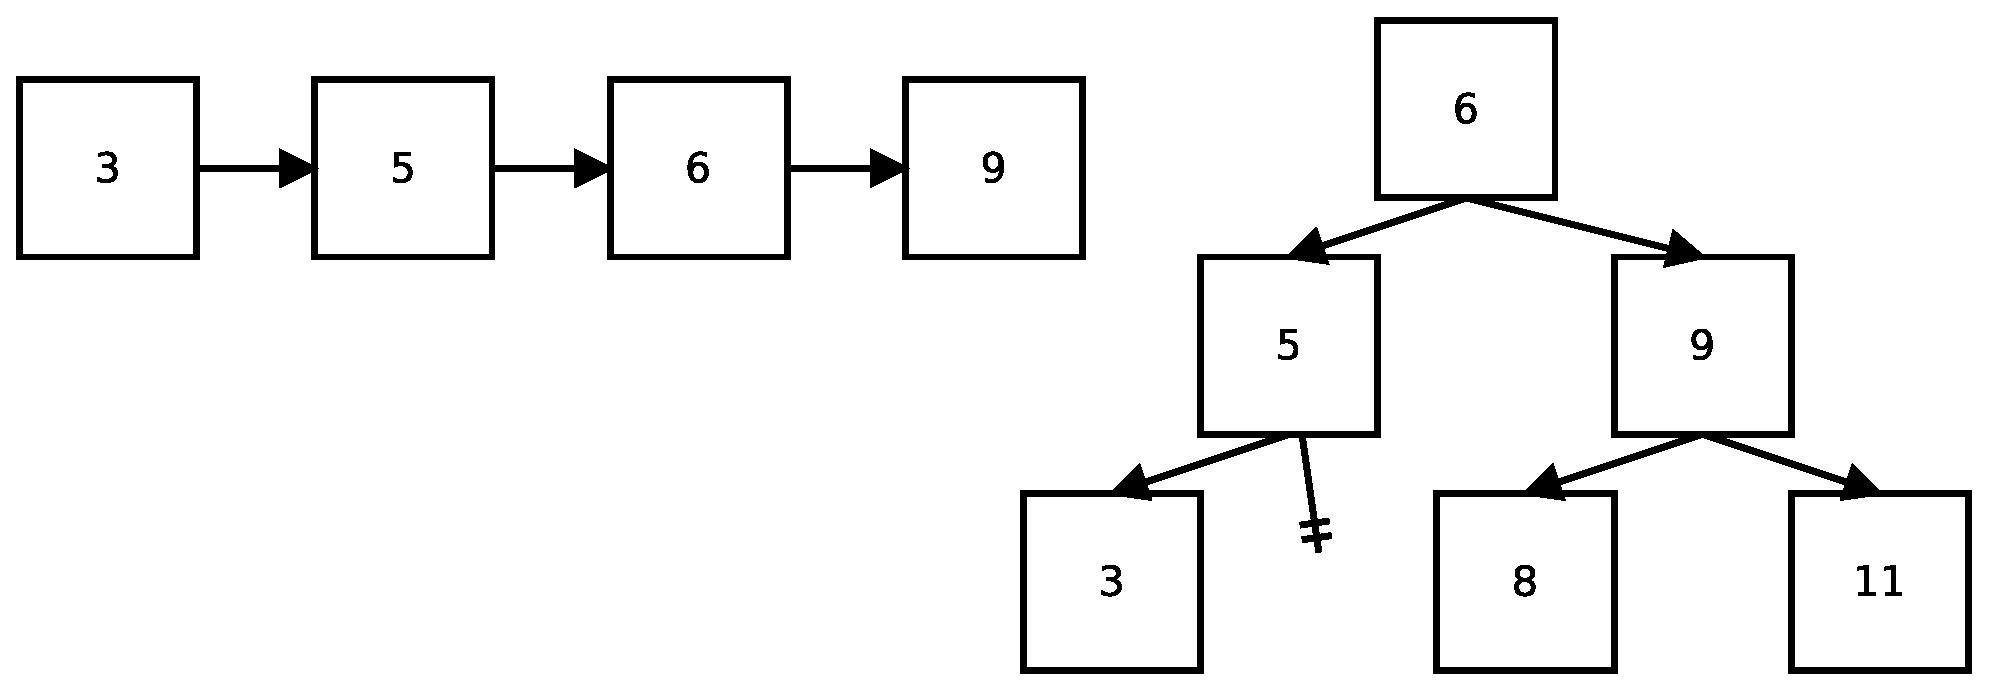
\includegraphics[width=\textwidth]{gfx/list-tree}
  \caption{In a singly-linked list, every element is connected to the next one. In a binary tree, every element is connected to two next elements.}
  \label{fig:listree}
\end{figure}

\begin{verbatim}
public class IntegerListNode {
    int value;
    IntegerListNode next;
    // ... methods would be here
}
(...)
public class IntegerTreeNode {
    int value;
    IntegerTreeNode left;
    IntegerTreeNode right;
    // ... methods would be here
}
\end{verbatim}

Trees where every node links to two other nodes are called
\emph{binary trees}. Binary trees are the most common types of
trees. But we can create trees of any cardinality:

\begin{verbatim}
public class IntegerTernaryTreeNode {
    int value;
    IntegerTernaryTreeNode left;
    IntegerTernaryTreeNode center;
    IntegerTernaryTreeNode right;
    // ... methods would be here
}
(...)
public class IntegerArbitraryTreeNode {
    int value;
    IntegerArbitraryTreeNode[] children;
    // ... methods would be here
}
\end{verbatim}

%%% Local Variables:
%%% mode: latex
%%% TeX-master: "main"
%%% End:


\chapter{Testing}
% Day 9,10: Testing (...whether they have learnt anything yet)
% Day 9:
% \item Software testing 
%       Show them the tests that test 
%         whether their versions work the
%         same as the versions of the Java library.
% \item NEXT YEAR: overloading of methods -> assertEquals()
% 
% IMPORTANT: HOW DO YOU RUN TESTS WITHOUT ECLIPSE (from cmd)!!
%    Easy: compile: javac -cp /.../junit.jar TestClass.java
%          run:     java  -cp
%          /.../junit.jar:. org.junit.runner.JUnitCore TestClass
% 
% \item Ultra-brief introduction to annotations in Java

\section{Software testing}
\label{sec:software-testing}

I know your code has bugs. If it is a small project it will have a few
bugs. If it is a big project it will have a lot of bugs. I know.

How do I know? Because I know you are a human being, and human beings
make mistakes. When a programmer is writing code there are too
many things to keep in the short-term memory at the same time: data
structures, communication between different parts of the program,
flows of information\ldots ~ Every program except the most trivial ones is
too complex for the human mind to see in its entirety. This is why we
use methods to isolate operations (using methods), and
why we use classes to group different behaviours and states in our program
around some conceptual ideas that we can grasp (e.g.~a supermarket has
queues, a queue has people, a person has a name and knows who is
behind in the queue; a company has products and employees, employees
have names and take money from the company, products give money to the
company). 

Structured and object-oriented programming are ways in which
programmers can reduce the complexity of their programs to levels that
are (more or less) manageable for their human minds, 
but it is still impossible to write
programs that do not contain bugs. Humans, even the best programmers,
have a tendency to forget some details of the program. That is the way
the human mind works: it concentrates on the most fundamental aspect
and forgets the details until needed\ldots which in computing means
when the program is already executing and nothing can be done about
it. 

Long story short, as long as programming is performed by humans,
programs will have bugs. The compiler can make sure that a program is
syntactically correct but it cannot tell if  it makes sense or
even whether it will do what the programmer expects. 

That is why software testing is important. Testing a program is a way
to ensure that the program does what it should. There are two types of
testing: manual and automatic (Table~\ref{tab:test}). You are already
familiar with the former type: you have been doing it for weeks, for
those programs you have been writing until now. Now we will learn how to
do things properly in an automated way. 

\begin{table}[htbp]
  \centering
  \begin{tabular}{|p{2.5cm}|p{5.8cm}|p{5.5cm}|}
    \hline
    & Manual & Automated \\
    \hline
    Speed & Very slow & Very fast \\
    Focus & Most important bugs known & Every single bug known \\
    Thoroughness & Sometimes forgets to test some things & Tests everything always \\
    It feels\ldots & Very repetitive and boring & Nothing: work is done by computer \\
    \hline
  \end{tabular}
  \caption{Manual testing vs automated testing}
  \label{tab:test}
\end{table}

\subsection{Automated testing}
\label{sec:automated-testing}

The idea behind automated testing is very simple: make a ``testing'' program that
verifies whether your ``main'' program behaves as expected. You can execute
this ``testing'' program every day as your original program grows to
make sure that everything works as it
should. Figures~\ref{fig:sdddfsdsrrers} and~\ref{fig:sdfsdsers} provide
two examples from real life when programs did not behave as expected. 

\begin{figure}[tbp]
\begin{verbatim}
    Programmer 1: The program has messed-up and now we have lost data
        from our clients!
    Programmer 2: How is that possible?
    Programmer 1: The function returnPastPurchases() returned null,
        the system got a NullPointerException and crashed. 
    Programmer 2: Oh! It returned null because there were no past
        purchases. 
    Programmer 1: But it has always returned an empty array! 
    Programmer 2: But I thought that null was more elegant than an
        empty array. If there is nothing to return, why not return
        null? 
    Programmer 1: What about... because the rest of the program
        expects an empty array! Now we face our clients sueing us!
    Programmer 2: I am sorry...
\end{verbatim}  
  \caption{Scenario 1: unmet expectations}
  \label{fig:sdddfsdsrrers}
\end{figure}

\begin{figure}[tbp]
\begin{verbatim}
    Programmer 1: Good, now we have found the bug. Method 
        getTaxReturns() had problems when it received a null
        TaxPayer. We have fixed the method that was returning 
        a null TaxPayer. Let's create a test for it to make sure it
        does not happen again. 
    Programmer 2: No need to. It will never happen again. I will never
        forget this week working 20h a day! I promise you no method
        will return a null TaxPayer ever again. 
    (...one year later...)
    Programmer 1: There is a serious bug in the system!
    Programmer 2: I have found it! Someone returned a null TaxPayer. 
    Programmer 1: What? A year ago, you promised me that it was not
        going to happen again!
    Programmer 2: It is not my fault! Someone else must have made
        changes to the core classes!
\end{verbatim}  
  \caption{Scenario 2: Star Bugs: Return of the Bug}
  \label{fig:sdfsdsers}
\end{figure}

Programs can behave badly for an infinite number of reasons,
including: 

\begin{itemize}
\item bad programmers writing bad code.
\item lack of communication between programmers in a big project.
\item programs without documentation that have to be modified, usually
  by a programmer that has nothing to do with the original
  programmers.
\item programs with \emph{obsolete} documentation that have to be modified, usually
  by a programmer that has nothing to do with the original
  programmers.
\item version changes in external libraries (or even the programming
  language) that are not backwards-compatible.
\item changes in one part of the program that affect some other part of
  the program, apparently unrelated. 
\end{itemize}

The last reason is particularly important because it is the most
common and it is quite difficult to fight. Big programs are usually
written by many programmers, and none of them knows everything about
the code. Sometimes a change in one region of the code breaks something
else that had been working seamlessly until then. The problem becomes worse as
programmers leave the project and other programmers join in with no
previous knowledge about the program. 
This results in programs that
are more and more difficult to modify and adapt as they evolve over
time. This is know as \emph{code viscosity}, and it is bad. Automated
testing, by means of regression tests, is a way of fighting code
viscosity: when the automated tests verify that everything 
is still working ---even those parts of the program unknown to the
programmer---, one can be confident that the last change did
not brake anything. 

\subsection{Creating tests}
\label{sec:creating-tests}

How do you write your own tests for your Java programs? You write them
as Java programs, using a special library called JUnit. There are
other ways, but JUnit is very simple, powerful, and well-known. JUnit
does not come with Java by default, but you can easily install it from
the web as it is free software\footnote{\emph{Free} as in free speech,
not free beer.}. 

An automated test is just a collection of methods that will be
executed by JUnit. These methods will test the methods in your
``main'' classes, and check that they return the right values. If they
do not, for any reason, JUnit will raise a flag so that you can look
into your code and find out why it is not behaving as expected. 

Let's see an example. Imagine that we have 
a method that returns the initials of a name
in a class called \verb+Person+: 

\begin{verbatim}
    public String getInitials(String fullName) {
        String result = "";
        String[] words = fullName.split(" ");
        for (int i = 0; i < words.length; i++) {
             String nextInitial = "" + words[i].charAt(0);
             result = result + nextInitial.toUpperCase();
        }
        return result;
    }
\end{verbatim}

A test program would be a Java class that could look like this: 

\begin{verbatim}
    import org.junit.*;
    import static org.junit.Assert.*;
    
    public class PersonTest {
       @Test
       public void testsNormalName() {
            Person p = new Person();
            String input = "Dereck Robert Yssirt";
            String output = p.getInitials(input);
            String expected = "DRY";
            assertEquals(output, expected);
         }
    }
\end{verbatim}

As you can see, there are several things that make a test class (using
JUnit) different from a normal Java class. First of all, there is no
main method. JUnit tests are not executed directly, they are executed
by JUnit, so there is no need for a main method. 

A second important difference are those \verb+import+ statements at
the beginning, before the class definition. These  statements
are the way in which a programmer can tell Java to use classes that
are not in the current folder (they must be in the \emph{classpath},
though). 

If you want to import just some \emph{static methods} from some
class, you can use \emph{static imports}. In this example, the method
\verb+assertEquals(String,String)+ is statically imported from class
\verb+Assert+. This is only a convenience so that you do not need to
write \verb+Assert.assertEquals(....)+ every time you need it, 
only the method's name is enough. 

The third difference is the most important one. There is a special
kind of word before the method definition, a word starting with an at
symbol: \verb+@Test+. These at-words are called \emph{annotations} in
Java, and have a special meaning for the compiler. In this case, the
annotation \verb+@Test+ tells JUnit that the method
\verb+testsNormalName()+ is a test to be run by JUnit. This is the way
JUnit knows which methods to run and which methods to ignore. (We will
learn more about annotations in the future). In short, you must
write \verb+@Test+ before each of your test methods. 

You can also appreciate some conventions in the code. The test class
for class \verb+Person+ is called \verb+PersonTest+ (some people
prefer \verb+TestPerson+). The method's name tells the story of
the test: it can be read as ``this method''\ldots \verb+testsNormalName()+:
this method tests a normal name. You can also appreciate some of the
variable names: \verb+input+, \verb+output+, \verb+expected+ (for
expected output). 

The tests ends with the method \verb+assertEquals(String,String)+,
statically imported from class \verb+org.junit.Assert+. This method performs an
\emph{assertion}, a test that the parameters verify some condition
(equality in this case). If that is not true, the method will throw an
exception and JUnit will report a failure in your test. Assertion can
be made on equality, difference, nullity, and truth value. The most
common methods are \verb+assertEquals()+, \verb+assertTrue()+, and
\verb+assertFalse()+. The full list
of methods of \verb+Assert+ can be found in the documentation of the
class\footnote{http://junit.sourceforge.net/javadoc/org/junit/Assert.html}. 

\subsection{Running tests}
\label{sec:running-tests}

To run your tests, you must run JUnit from the command
line\footnote{In the future, we will learn how to do this
  automatically from an IDE like Eclipse, but for now we will make the
effort of understanding each step by itself.}. In order
to do so, you must bear in mind some facts: 

\begin{itemize}
\item JUnit is not part of core Java, so it must be added to the
  \emph{classpath} either manually or by modifying the environment
  variable CLASSPATH.
\item When you modify the CLASSPATH, you must remember to add the
  current folder (or Java will not find your class!).
\item The core class in JUnit is called, perhaps unsurprisingly,
  \verb+JUnitCore+. 
\end{itemize}

With this in mind, you are now able to run the following
command: 

\begin{verbatim}
    > javac -cp .:junit-4.10.jar PersonTest.java
\end{verbatim}

This will compile your test class(es). The \verb+-cp+ parameter is the
way you can modify the classpath when executing \verb+javac+ or
\verb+java+. Remember that elements in the classpath are separated by
colons~(:) on Linux and Mac, but they are separated by semicolons~(;) on
Windows. To run the tests, you must execute the main method in class
\verb+JUnitCore+, which is inside package \verb+org.junit.runner+,
passing all your test classes as parameters: 

\begin{verbatim}
    > java -cp .:junit-4.10.jar org.junit.runner.JUnitCore PersonTest
\end{verbatim}

You can read that as ``execute on the Java Virtual Machine'', using as
classpath both the current folder~(.) and the JAR file of
JUnit\footnote{If you have left the JAR file, your classpath will look
different. You must write the full path to your JAR file in the
classpath.}, the
main method of class \verb+org.junit.runner.JUnitCore+ and pass as
argument the string ``PersonTest''. This will make JUnit run all the
tests inside the class PersonTest (as marked by the \verb+@Test+
annotation). 

If all tests run successfully, JUnit will congratulate you. If one or
more of the tests fail, JUnit will inform you of which tests failed
and why. 

\subsection{Designing tests}
\label{sec:designing-tests}

So far we have seen how to create automated tests, and how to execute
them in order to find bugs in our \emph{production code} (i.e.~our
``main code'', the program that we are creating to solve a
problem). Programmers usually create a lot of tests to verify the
behaviour of their classes (i.e.~as defined by its public methods, its
interface). 

But there is something that we need to bear in mind at all
times: tests do \textbf{not} prove that your code does not contain
bugs. No matter how many tests you have written, no matter how many
cases you cover with them, there is no way to prove that a code does
not contain bugs. We can only try to push the chance of bugs as low as
possible, but it is never zero.

You can think of tests as torches in a cavern, where the cavern
represents your code. The more
torches you place in the cavern, the more light there will be, so there
will be fewer shadows where bugs can hide. But you must place your
torches carefully. If you just put a lot of torches in one place, most
of the cavern will be in shadows, and your bugs will lurk in there until
the time is right to appear (usually to make your company look bad or
lose money or both). If you place your torches carefully and
illuminate as many corners as possible, your bugs will find it more
difficult to hide undetected. How can we ensure that we keep our
cavern as illuminated as possible? There are three basic strategies.

\subsubsection{Testing basic functionality}
\label{sec:test-basic-funct}

The first tests that you must write, the first torches you have to
place in your cavern, are those that shed light on the main features
of your code: if you have written a class with a method that returns
the number of colours in an image, write a test that provides an image
and checks that the right answer is returned; if you have written a
method that returns the initials in a name, write a test that checks
that the right initials for a name are returned. 

This is the simplest strategy, and everybody has it in mind, so there
is no need to hammer it anymore. The next two strategies are usually
forgotten by many programmers, so it is important that you think about
them carefully. 

\subsubsection{Testing border cases}
\label{sec:testing-border-cases}

Good code is simple, clear, and general. Programmers create programs
that repeat the same operations most of the time: checking the
salaries of all employees in a company, verifying the medicine doses
of all patients in a hospital, calculating all stress tensors for
every point on the wing of a plane, etc. Usually, this is performed
correctly in most programs. If it is not, the error tends to be quite
evident and is detected with the simple
``basic'' tests (or even at compile time).

Basic functionality is not the main source of bugs. 
Programs have a tendency to break around the \emph{borders}. Using the
metaphor of the cave, you can think that corners are usually darker
than the rest of a cave room, so they are good hiding places for
bugs. Border cases (the first, the last, etc) are usually slightly
different from the general case and your implementation may break
there: a list may not remove the first element correctly, or the
last; a loop may not check the last element in a list, or go out of
bounds; a method may break when it is given an empty list as a
parameter (or null). 

Border cases must always be checked in your tests. This is very
important. Leaving corners and borders in the shadows is just a
disaster waiting to happen. Many programmers forget to test border
cases and are later surprised by bugs in a code that seemed to be
``working fine''.

\subsubsection{Find bugs once}
\label{sec:find-bugs-once}

This is the most important rule in software testing, yet it is usually
forgotten by many programmers (especially lazy programmers). Whenever
you find a bug in a code, and you will find many in your life as a
programmer, you have to follow this simple algorithm: 

\begin{enumerate}
\item Find the bug again. Repeat the same steps until you know exactly
  how and when the bug appears. This is called
  \emph{reproducing the bug} and it is not always easy in large,
  complicated programs.
\item Once you have been able to reliably reproduce the bug manually,
  write a test that reproduces the bug programmatically. Check that
  the bug is always fired when you run your test with JUnit. Make the
  test as simple as possible.
\item Once you have written the simplest test that reproduces the bug
  ---\textbf{and only then}--- fix the bug. Verify that the tests passes. 
\end{enumerate}

Following this simple algorithm will ensure that the same bug does not
appear again and you never find yourself in the situation described in
Figure~\ref{fig:sdfsdsers}. You are a human being and you make mistakes. No
matter how careful you are, your code will have some bugs. Most of the
time you will find bugs in code that was written by other programmers
that were not as careful as you. Following the ``find bugs once''
algorithm will at least ensure that you do not have to track the same bug
twice and repeat work you have already done. This is a algorithm to make
sure your projects only move forward, never backwards, and you do not
waste your precious time. 

\subsection*{Final note: Running tests overnight}
\label{sec:runn-tests-overn}

The good thing about automated tests is that you do not need to run
the tests yourself over and over again. You write the tests and then
tell JUnit to run them. Every day, you can tell JUnit to run every
single test that you have written so far. Serious professional
projects have thousands or millions of tests: no human being can do
all of that without dying of boredom. That is why automated testing is
important. 

Testing everything frequently ensures that the code does not go
backwards, e.g.~that introducing new features does not break other
features that were already working. This why it is sometimes called
\emph{regression testing}: it makes sure that the code does not
regress, i.e.~it does not go backwards. 

It is common for most professional projects to run \emph{all tests}
on a daily basis, usually overnight when the programmers involved are
sleeping\footnote{Well, most of them at least.}. This is done by means
of an automatic script that retrieves the sources from a public
repository (e.g.~on GitHub), compiles everything, and then runs all
the regression tests. If anything is wrong, the programmers can fix it
as soon as they are back to their computers. Usually programmers run
a subset of all tests before pushing their changes, but a serious
project can have millions of tests that take several hours to run;
therefore, a full comprehensive test run is necessary every day to
keep projects on track. 

% How to design your tests
%   - check basic functionality
%   - check border cases
%   - Find bugs once
%     - the second test
%  @Test
%    public void trySG_S()
%      {
%         T t = new T();
%         String input = "Dereck Robert  Yssirt";
%         String output = t.getInitials(input);
%         String expectedOutput = "DRY";
%         assertEquals(output, expectedOutput);
%      }


%%% Local Variables:
%%% mode: latex
%%% TeX-master: "main"
%%% End:

% 
% Day 10:
% \item final
% \item Test-driven development
%       Show them the tests that test whether their versions work the
%       same as the versions of the Java library.
% \item Ultra-brief introduction to annotations in Java
% \item Annotations to cover:
%     @Test
%       timeout = 15000
%       expected = IllegalStateException.class
%     @Before, @BeforeClass
%     @After, @AfterClass
% \item JavaDoc: do you want your classes to look like the
%      proffesional ones? Use Javadoc!!
% \item Do not confuse annotations with JavaDoc!! @throws, etc
% \item final
% \item Introduction to the Java Collections library
%
% ASSIGNMENT: produce a test specification for some program, and then
% create the program... maybe better give them the interface and then
% they must implement the battery of tests... mmm... difficult to
% test, isn't it? How do you test tests? On the other hand, this is
% important stuff so they should be examined on it...
% 
% FOR NEXT YEAR: refactor TDD into D9, and leave D10 with little extra
%     material (or no extra material whatsoever, apart from the
%     collection library and JavaDoc?)

\section{Constants}
\label{sec:constants}

Programs use data, lots of data. Data is stored in variables of simple
and complex types, the latter being pointer that point to objects in
the memory. We have used a lot of variables up to now. 

Sometimes, we know that a piece of data is not going to change over
the course of the program. Maybe it is a physical constant like the
speed of light, maybe it is a mathematical constant like $\pi$, maybe
it is another element of your program that you know will never
change. 

Moreover, you want your program not to allow any part
of the code (possibly \emph{buggy}) to modify it. This is achieved by
using the keyword \verb+final+. This keyword tells Java that the value
of a variable must never change from the moment it is initialised
until the program ends. See an example: 

\begin{verbatim}
    public static final double PI = 3.14159265359; 
\end{verbatim}

% Cross-refs
You remember that we said that static \emph{fields} should be used
sparingly, and mostly (or only) for constants. The keyword
\verb+final+ is used to declare an identifier as constant, and
therefore both keywords are frequently found together when applied to
fields. 

You may also remember that we mentioned that constants fields can be
made public, as there is no risk of someone modifying their values and
having undesirable side effects. If you ever make a field public in a
class that has methods, make sure you make it static and (especially)
final too.

\section{Documenting your code with JavaDoc}
\label{sec:docum-your-code}

% TODO: write this better

We have already seen how the Java library is completely documented
online. All classes explain what they are and what they do (i.e.~their
methods, explaining the parameters), and this information is online on
the Java API documenation of JavaDoc. You can find the JavaDoc easily
by typing ``Java API'' on your favourite search engine. 

The good news is that it is easy to document your own classes in the
same professional way as the core Java library. In order to do so, we
just need to write the comments of our code in a special way and then
use the program \verb+javadoc+. 

\subsection{How to write comments}
\label{sec:writing-comments}

As we briefly saw when we introduced interfaces, JavaDoc comments
start by \verb+/**+, end by \verb+*/+, and can span several
lines. JavaDoc comments can also tag additional information regarding
parameters or return values, as shown in the following example: 

\begin{verbatim}
    /**
     * An StringStack is a dynamic structure that can contain any number
     * of strings. 
     * 
     * New elements (i.e. Strings) can be put on top of the stack or
     * removed from the top of the stack. Only the element at the top of
     * the stack can be removed at any given time; to access a specific 
     * element, all elements on top of it must be removed (popped) first. 
     * 
     * This interface allows the user to look at the elements of the list
     * even if they are not accessible. 
     */
    public interface StringStack {
        /**
         * Put an element at the top of the stack. 
         *
         * @param newString the new string to be put
         */
        void push(String newString);
        /**
         * Removes the element at the top of the stack and returns it. 
         *
         * @return the element at the top of the stack
         */
        String pop();
        /**
         * Replaces every occurrence of one string in the stack
         * for another string. 
         *
         * @param oldString the string to be replaced
         * @param newString the new string to replace it with
         */
        void push(String oldString, String newString);
    }
\end{verbatim}

There are three important things to notice in this example: 

\begin{itemize}
\item All comments start with \verb+/**+ and end with \verb+*/+. It is
  customary to make each line in the comment start with a star too.
\item Parameters are documented with the tag \verb+@param+, followed
  by the name of the parameter, followed by the description.
\item Return values are documented with the tag \verb+@return+,
  followed by the description of what is returned. 
\end{itemize}

Comments should explain the functionality of your classes and methods
in a short and clear way. Comments should not explain the internal
implementation details unless it really makes a difference to other
programmers using those classes or methods. In other words, comments
should be as clear as possible, and as short as possible, in that
order of importance. 

\subsection{How to create the online documentation}
\label{sec:how-create-online}

Creating the webpages with the documentation of your classes and
methods is very simple. Assumming that you have all your classes
documented (i.e.~with proper comments) in a folder called \verb+src+
and want to put all the web pages in a folder called \verb+www+, you
just need to run the following command: 

\begin{verbatim}
    > javadoc path/to/src/*java -d path/to/www/
\end{verbatim}

This will generate all the web pages, HTML files, CSS style sheets,
links, etc, for you. 

\section{More on testing}
\label{sec:more-testing}

\subsection{Additional annotations}
\label{sec:addit-annot}

In the former section we have seen how basic testing is performed. A
testing method is marked with the annotation \verb+@Test+, and this
indicates to JUnit that the method will be run as a test. The testing
method contains one (sometimes more) \emph{assertion}, which is
nothing more than a call to one of the methods of class
\verb+or.junit.Assert+, maybe \verb+assertTrue(boolean)+. 

In this section we are going to learn how to create slightly more
complicated tests. 

\subsubsection*{Constraints: timeout and expected}
\label{sec:timeout}

Sometimes a bug does not result in a bad result being returned,
sometimes it results in an infinite loop or an extremely long response
time. If we want to specify a maximum time for our testing methods to
run we can do it by passing a ``timeout'' parameter to annotation
\verb+@Test+, as in the following example: 

\begin{verbatim}
    @Test(timeout = 1000)  
    public void testsThatFinishedBeforeOneSecond() {  
        // ...
    }  
\end{verbatim}

If the method does not return a value before 1000 milliseconds have
passed, the test will fail. 

We can also expect a method to return an exception, as in the
following example: 

\begin{verbatim}
    @Test(expected = IndexOutOfBoundsException.class)
    public void testsNegativeIndecesFail() {  
        // ...
    }  
\end{verbatim}

If the method does not throw an \verb+IndexOutOfBoundsException+ in
this test, the test will fail. Note that this is quite the contrary of
the usual behaviour: when a testing method throws an exception, it is
usually a symptom of something not working as expected; but this not
always the case. Situation in which we may want to expect an exception
include requests to lists beyond their size, parsing strings that
are not in the right format, and passing negative parameters to
methods that only accept positive integers. 

\subsubsection*{Initialisation: Before and After}
\label{sec:init-before-after}

Testing methods usually require the creation of some object. It is
quite common that this is needed for all testing method in a testing
class. 

Instead of repeating the same code in each and every method, which
each boring and error-prone, we can create a method to that before
every testing method is called. This method must be annotated with
\verb+@Before+. In the same way, if some cleanup must be performed
after each testing method ends and before the next testing method
starts, this should be marked with the \verb+@After+ annotation. See
the example: 

\begin{verbatim}
    @Before
    public void buildUp() {  
        // A file is created here to be used in every test. 
    }  
    @After
    public void cleanUp() {  
        // The file is deleted here, after each test ends
    }  
\end{verbatim}

Assuming that your testing class contains three testing methods, the
execution path would be: buildUp, first test, cleanUp, buildUp, second
test, cleanUp, buildUp, third test, cleanUp. Note that you can change
the names of the methods (buildUp and cleanUp are common choices).

\subsubsection{Heavy initialisation: BeforeClass and AfterClass}
\label{sec:heavy-init-befor}

Using \verb+@Before+ and \verb+After+ is appropriate in those cases in
which initialisation and clean-up are fast. However, if the resources
needed are costly to allocate and release, and if they are not changed
inside each testing method, then it is better to just do some
initialisation at the beginning of all tests and some clean-up at the
end of all test. 

This is done by using the annotations \verb+BeforeClass+ and
\verb+AfterClass+. Examples of resources that are acquired and
released once per class include network connections and database
connections. 


\subsection{Test-Driven Development}
\label{sec:test-driv-devel}

Test-Driven Development (TDD) is a programming methodology that advocates
that tests should be driven before the actual program. This is
radically different from writing the program first and then writing
the tests as we have done in the past.

The TDD methodology consists of three steps that are repeated in a
loop: 

\begin{enumerate}
\item Write the tests for the next functionality of the program. Make
  sure they fail. If they do not fail, that means they are not testing
  anything that was not tested before (and are redundant) or they are
  incorrect (and should be fixed). 
\item Write the minimal code that passes all the new tests.
\item Refactor the code to make it clearer and simpler. Run the tests
  at the end to make sure the final functionality is right. 
\end{enumerate}

There are several benefits for programming in this fashion: 

\begin{itemize}
\item As the tests are written in advance, the \emph{production} code
  is written in a way that is easy to test.
\item As the tests are written in advance, all the code is tested by
  at least one testing method. Otherwise, programmers can forget to
  test some methods.
\item Writing the tests first makes the programmers think about the
  real specification of the class or method, focusing on \emph{what}
  needs to be done before their short-term memory is filled with
  \emph{how} to do it.
\item Errors are detected early, when they are cheap to fix. It is
  more difficult for bug to remain undetected until later in the
  development, when it can be more costly to fix them.
\end{itemize}

This methodology can be combined with the ``find bugs once'' strategy
we already know. A program can be developed using TDD, finding most
bugs in the process, but some bugs may appear later in the development
cycle; if that happens, the ``find bugs once'' strategy results in
adding new tests that will find them as soon as they reappear.


%%% Local Variables:
%%% mode: latex
%%% TeX-master: "main"
%%% End:


% Day 11,12: Padding week to recover their breath
% \item Introduction to generics in Java
%    Make your own List<T> (and Node<T>), Stack<T> and Queue<T>
%    (probably extending List<T>), and Map<K,V>
% \item Introduction to the Java Collections library
% \item More on object orientation: inheritance (and type
%   hierarchies, upcasting/downcasting of complex types),
%   polymorphism, overloading, overriding, "static" (good "real"
%   example: implementation of 
%   read-only versions of collections), interfaces (like Iterable, 
%   Runnable, or the ones in the Collections)... and why interfaces
%   are important. 
% \item the keyword super, and its role in constructor methods:
%     "hidden" super()
% \item the final keyword for methods and classes
% \item more on .equals(), .hashcode(), etc
% \item Annotation @Override
% Day 11: 
%    - extends
%      - top-down inheritance: interfaces + code = abstract classes
%        - explain that abstract classes are "extended" and have
%          "abstract" methods
%      - bottom-up inheritance: abstract/non-abstract classes
%      - extension of already existing classes
%         - final for methods and classes
%      - everything is Object
%    - overriding / overwriting
%      - annotation @Override
%      - equals(), hashcode()
%    - super
%      - "hidden" super()
%    \item composition better than extension
\section{Inheritance}
\label{sec:inheritance-1}

Repeating code is a bad thing. If the same code is used in more than
one place in a program, that is a disaster waiting to happen. Sooner or
later, one of the copies of the code will be changed (probably to fix
a bug), but not all copies will be changed\ldots and unpredictable things
will happen (never good). 

We already know one strategy to prevent code repetition: using methods 
inside a class. By enclosing code inside a method, the
programmer can just call the method from any other section of the code
and the same instructions will always be executed (probably with
different values for the parameters). In this section, we will move
one step further to avoid code repetition by using \emph{inheritance} to
prevent code repetition \emph{among} classes. 

\subsection{Extending already-existing classes}
\label{sec:extend-alre-exist}

From all the forms of inheritance, the easiest to understand is the
extension of already existing classes. This is done by means of the
keyword \verb+extends+. You can think of this keyword as stating a
``is a'' relationship: you use it to say that objects of your class
are also objects from another class\ldots with something on top.

Let's assume that we had a class \verb+Ebook+,
part of a program to run an electronic book reader. The class would
have
several methods, including some like \verb+nextPage()+,
\verb+prevPage()+, and maybe even \verb+readAloud(int page)+. When the next
version of our electronic book reader comes out, it includes a new
feature to regulate the background light of the screen. At this point
we have at least two options. First, we can add a new method
\verb+setLight(int)+ to the \verb+Ebook+ class to regulate the
background light; however, this method would also be included as part of the
software running in all the ``plain with no light'' e-books.
A second possibility, is to create two different classes,
\verb+Ebook+ and \verb+LightEbook+, each of them being used for a different
hardware; but this would lead to having lot of methods repeated in
both classes (e.g.~\verb+nextPage()+), which is
bad. 

There is a third, much better possibility. We can make
\verb+LightBook+ extend \verb+Ebook+, as in the following example code 
(JavaDoc comments ommited for the sake of brevity): 

\begin{verbatim}
    public class LightEbook extends Ebook {
        private int lightLevel = 100;
        public void setLight(int newLevel) {
            this.lightLevel = newLevel;
        }
    }
\end{verbatim}

You can see that extending a class is very easy: just say that you are
extending it (in this example, ~\verb+extends Ebook+).
From that point on, your class will be able to use all the public methods (and
some more, see below on Section~\ref{sec:protected-keyword}) from
the class that you are extending without the need to implement them
again. In other words, you can call \verb+nextPage()+ on a
\verb+LightEbook+ object exactly in the same way as you would do it
on a \verb+Ebook+ object. 

The base class that is extended is called the \emph{parent class} or
\emph{superclass}\footnote{In this context, ``super'' is as in Latin,
  meaning ``up''; there are no connotations of big, extra, or more
  powerful. Remember that the convention in computing is that general
  classes or interfaces are ``up'' and more specific or extending classes
  are ``down''.}, 
while the extending class is called a \emph{subclass}. When there are
many levels of hierarchy (a class extends a class that extends another
class, etc), those classes up in the hierarchy are called
\emph{ancestor classes}, while those down in the hiearchy are called
\emph{descendant classes}. 

\paragraph{Everything is an object!}
\label{sec:everything-an-object}

In Java, every class extends class \verb+Object+ or descends from a
class that extends \verb+Object+. \verb+Object+ is a class from the
core Java library that provides a few methods that every other class
can use. The most commonly used is \verb+equals()+, which compares two
objects and returns \verb+true+ if they are the same (according to
some class-specific rules) and \verb+false+ otherwise. 

As everything is an \verb+Object+ by default, you do not need to write
it explicitly (\verb+...extends Object+): Java will do it for
you. Programmers must only explicitly say which class they are
extending if they are extending a class that is \emph{not} \verb+Object+.

\begin{verbatim}
    public class MyClass {  // no need to say "extends Object" here
        // ...              
    }
\end{verbatim}

\paragraph{Final classes}
\label{sec:final-classes}

You remember that we could use the keyword \verb+final+ to indicate
that a variable holds a constant value, i.e.~that the variable could
not be changed. In a similar way, we can use \verb+final+ to tell the compiler
that a class cannot be changed either. A class defined as \verb+final+
cannot be extended; trying to do so will result in an error at compile
time. 


\subsection{Top-down inheritance}
\label{sec:top-down-inheritance}

We have already seen that we can use \emph{interfaces} to specify what a
class is like or, in other words, what is its behaviour, i.e.~the methods
that are public and can be used by other classes. For example, we may
have an interface \verb+Animal+ that was implemented by classes
\verb+Dog+, \verb+Human+, and \verb+Horse+. The interface may define
methods like \verb+move()+, \verb+makeSound()+, and
\verb+breath()+. The three classes would each implement each method. 

It is quite possible that the implementations of movement and
sounds are quite different, but on the other hand it seems likely that
\verb+breath()+ is very similar (or exactly the same) in the three
classes. As we know, repetition of code is bad: if we have a bug
in the \verb+breath()+ method, we will be in trouble if we forget to
fix it in all classes. It would be much better if we could have the
same method in just one place so that each class could use it, in the
same way that the code in a method can be used from anywhere in the
class. 

In cases like this one, it would be great if we could put the 
real code in the interface, not just the declaration; then, all
classes would have it\ldots Well, it turns out we can do something like
that in Java. Although we cannot write any code in an interface, 
we can transform the interface into an \emph{abstract class}, and then
make the other classes \emph{extend} it. Let's see an example: assuming
that the original interface looked like this (JavaDoc comments ommited
for the sake of space):

\begin{verbatim}
    public interface Animal {
         void move(int meters);
         String makeSound();
         void breath(int air);
    }
\end{verbatim}

\ldots if we implement the method \verb+breath()+, the resulting
abstract class could look like this: 

\begin{verbatim}
    public abstract class Animal {
         private int oxygen = 0;

         public abstract void move(int meters);
         public abstract String makeSound();
         public void breath(int air) {
             this.oxygen += air / 4;
         }
    }        
\end{verbatim}

As you can see, there are many differences between an interface and an
abstract class: 

\begin{itemize}
\item First and foremost, an interface never contains any actual code,
  while an abstract class ---like any other class--- can contain real
  implementation, i.e.~statements that perform some actions.
\item Interfaces are \emph{implemented}, while abstract classes are
  \emph{extended}.
\item All methods in an interface are by definition public and
  abstract (i.e.~without actual code), so there is no need to write it
  down (but it can be done). On the other hand, methods in an abstract
  class can be private or public, abstract or not, and it must be said
  explicitly for each of them (see \verb+move(int)+, for example).
\item Abstract classes can contain mutable fields. All fields on an
  interface are by definition static and final (i.e.~constant).
\end{itemize}

There are also some similarities: 

\begin{itemize}
\item Both abstract classes and interfaces can be used as data
  types to \emph{declare} a variable of a complex type 
  (e.g.~\verb+Animal indiana = new Dog()+).
\item Neither can be used to \emph{instantiate} an object using \verb+new+
  (because neither contains a full ``blueprint'' of what the new
  object would look like, e.g.~\verb+new Animal()+ is not valid). 
\end{itemize}

\subsection{Bottom-up inheritance}
\label{sec:boot-up-inher}

Sometimes, inheritance is a consequence of the design of your
program: you have an interface (e.g.~\verb+Animal+) 
that is implemented by several classes (e.g.~\verb+Horse+, \verb+Dog+)
and then decide to add a little code into it and turn it into an
abstract class. 

Sometimes it happens the other way around: you have two or
more classes that are apparently unrelated, and then realise that they
have the same code. At this point you want to move the code ``up'' to
an abstract class. For example, imagine that we had a class
\verb+ManorHouse+ and another class \verb+Castle+, initially unrelated
in the design of our program: 

\begin{verbatim}
    public class ManorHouse {
       private Gate gate;
       // ...
       public void closeForTheNight() {
           gate.moveInwards(90);
           gate.getLock().setLocked(true);
       }
       // ...
    }
    (...)
    public class Castle {
       private Gate gate;
       // ...
       public void closeForTheNight() {
           gate.moveInwards(90);
           gate.getLock().setLocked(true);
       }
       // ...
    }       
\end{verbatim}

Code repetition is bad. As soon as we realise that both classes have
the same method, such method should be put in a parent class: 

\begin{verbatim}
    public abstract class GateGuardedBuilding {
       private Gate gate;
       // ...
       public void closeForTheNight() {
           gate.moveInwards(90);
           gate.getLock().setLocked(true);
       }
    }
    (...)
    public class ManorHouse extends GateGuardedBuilding {
       // ...
    }
    (...)
    public class Castle extends GateGuardedBuilding {
       // ...
    }       
\end{verbatim}

Now the method \verb+closeForTheNight()+ is available to both
\verb+ManorHouse+ and \verb+Castle+ because they are extending
the parent (abstract) class \verb+GateGuardedBilding+. 

Clear? Not so easy\ldots There are situations in which 
this ``repetition of code'' is not straighforward. Look at the
following simplified example:  

\begin{verbatim}
    public class DrinkRefrigerator {
        // ...
        public int buyCan(int money) {
           if (money < price) {
               return money;
           } 
           int change = money - price;
           releaseCan();
           return change;
        }
        // ...
    }
    (...)
    public class ChocBarVendingMachine {
        // ...
        public int getBar(int moneyGiven) {
           if (moneyGiven < price) {
               return moneyGiven;
           } else {
               giveChocolateBar();
               int change = moneyGiven - price;
               return change;
           }
        }
        // ...
    }
\end{verbatim}

Although it may not seem at first that a \verb+DrinkRefrigerator+ and
a \verb+ChocBarVendingMachine+ have much in common, an analysis of the
code of methods \verb+buyCan()+ and \verb+getBar()+ shows a strong
similarity, suggesting that the code should be abstracted away to a
parent class. How would it look like? Maybe something similar to this: 

\begin{verbatim}
    public class Sale {
        public boolean sold; // public fields because it does not
        public int change;   // have methods
    }
    (...)
    public abstract class VendingMachine {
        // ...
        public Sale buy(int money, int price) {
           Sale result = new Sale();
           if (money < price) {
               result.sold = false;
               result.change = money;
           } else {
               result.sold = true;
               result.change = price - money;
           }
           return result;
        }
        // ...
    }
    (...)
    public class DrinkRefrigerator extends VendingMachine {
        // ...
        public int buyCan(int money) {
           Sale sale = buy(money, price);
           if (sale.sold) {
               releaseCan();
           } 
           return sale.change;
        }
        // ...
    }
    (...)
    public class ChocBarVendingMachine extends VendingMachine {
        // ...
        public int getBar(int money) {
           Sale sale = buy(money, price);
           if (sale.sold) {
               giveChocolateBar();
           }
           return sale.change;
        }
        // ...
    }
\end{verbatim}

The code in the subclasses is shorter and clearer because all the hard work
is done in the code that has been abstracted and put in the parent
class. If this code was more complicated and involved several
comparisons or long intrincated calculations, the benefits would be
even greater. 

In this second example, it is important to note
that the ``repeated'' methods had two effects: a return value
(to give change) and a side effect (release can or chocolate bar). Because of
this, we needed to create a new intermediate class \verb+Sale+ ---with
no methods--- in order to be able to return two values from the new
method \verb+buy()+. Remember that methods can only return one value;
the only way they can return more is by using a complex type to
encapsulate them all. 

\subsection{Visibility revisited}
\label{sec:protected-keyword}

As it evolves and grows, a program can become really complex, usually
beyond of what its programmer(s) can cope with. We know that one of
the basic strategies to keep complexity under control is by hiding
information. 

Information is hidden by making it not visible: visible fields can be
read and written, but non-visible fields cannot; visible methods can
be called, but non-visible fields cannot.  We have used two keywords
to control the visibility of our classes' fields and methods:
\verb+public+ and \verb+private+. Although these two keywords will
cover most of your needs as a programmer, it is good to know that
there are four levels of visibility in Java: public, protected,
default (package), and private.

\subsubsection{Public}
\label{sec:public}

Public fields are visible for any other class, and can be read and
written accordingly. Letting other classes (even classes that you have
written yourself) to modify
the fields of your classes can have unpredictable effects in a
normal-size program, and that is why you should make all your fields
private as a rule of thumb. The only exception are the fields of
method-less just-used-as-intermediate-data classes (like \verb+Sale+
in the former section). 

Public methods are visible to other classes and define the public
interface of your class. This is usually made explicit by implementing
one or more Java interfaces. Note that there is an ambiguity in
natural language here: the public methods of a class are its ``interface''
in the sense that they define how other classes can interact with it,
but that does not necessarily mean that the class \verb+implements+
(in the Java sense) a explicit Java \verb+interface+ defined in a
\verb+.java+ file. You should keep this distinction clear when you
read the documentation of software projects as both meanings of the
words are sometimes used without much care. 

\subsubsection{Protected}
\label{sec:protected}

Protected fields and methods are visible for classes in your package
(i.e.~the same folder/directory as the class) and for descendant
classes. There are a few cases in which the distinction
\verb+protected+ vs. \verb+public+ makes sense (i.e.~in event-oriented
architectures) but in most cases this nuance is not worth the
additional complexity, and that
is why many of the most recent programming languages do not include a
\verb+protected+ visibility, only \verb+public+. 

As a rule of thumb, use always public if you want other classes to
call the methods in your class. On the other hand, it is important to understand
what \verb+protected+ means because you will find it often when you
read Java code, especially if it is old legacy code. 

\subsubsection{Default (i.e.~package)}
\label{sec:default-i.e.-package}

When the visibility of a field or method is not specified, its default
visibility is ``package-wide'', i.e.~it is visible to other classes in
the same package. There is not a keyword for declaring ``package''
visibility: fields and methods of unspecified visibility become
visible for other classes in the same package. 

Up to now, you have not noticed any difference
between \verb+public+ visibility and default visibility because all
your interacting classes have been part of the same package or were
part of the standard Java library (e.g.~String) and you used only
their public methods. 

When Java was originally created, making things visible to the same
package seemed like a good idea for several reasons. However, things
have changed over the years and it is very rare today to find a
situation where ``package'' visibility makes sense but \verb+public+
visibility does not, with the additional complexity of keeping track
and what is visible at which level. Therefore, you will very rarely
find default visibility in Java code for a good reason; on the
contrary, it is almost
always a symptom of sloppy programming, a sign of a programmers not
thinking properly about the design of their program or --even worse---
not understanding the difference between \verb+private+ and default
visibility.   

\subsubsection{Private}
\label{sec:private}

Private fields and methods are only visible inside their own class. This
is the most complete form of ``hiding'', and should be the default
option for all the fields and most of the methods (unless they are
defined in an interface, i.e.~they are useful for other classes). 

Note that \verb+private+ only determines visibility between \emph{classes},
not between \emph{objects}. Objects of the same class are able to see each
other fields and methods. This is very evident in most implementations
of the \verb+.equals()+ method. 

\begin{verbatim}
    public class Integer {
        private int value;
        // ...
        public boolean equals(Integer other) {
            if (this.value == other.value) {
                return true;
            } else {
                return false;
            }
        }
    }
\end{verbatim}

Although the field \verb+value+ is private and cannot be seen from any
other class, any object of class \verb+Integer+ can see the
\verb+value+ method of other objects of the same class. 

\subsection{Changing behaviour, overriding methods}
\label{sec:chang-overr-behav}

Extending a class is a way of reusing part of its code in the form of
its public methods. However, there are cases in which by extending a
class you are inheriting a method you do not want. For example, your
class \verb+Employee+ may inherit from class \verb+Person+ a method
\verb+equals()+ that says that two objects are the same person if they
have the same passport number; however, you want your employee-objects
to represent the same employee if they have the same national
insurance number. When this happens, you have to \emph{override} the
method. 

Overriding a method is trivially easy: just write the method
again. Java will automatically use the most specific version of the
method when the method is called. Methods \verb+equals()+ and
\verb+hashcode()+, from class \verb+Object+, are typical examples of
methods that are overriden by many classes. 

\begin{verbatim}
   @Override
   public boolean equals(Object other) {
        // ... different code here to establish equality
   }
\end{verbatim}

The \verb+@Override+ annotation\footnote{We will see more about
  annotations in a week, when we start doing automated testing. For
  now, you just need to know that they are added just before the
  method declaration and start with a @ sign. } is optional, but it is a good idea to
always use it. This will make it evident to other programmers 
that the method is overriding a
method from an ancestor class. 

% TODO: Remove Footnote

\paragraph{Final methods}
\label{sec:final-methods}

In the same way that we can declare a class to be \verb+final+ so that
it cannot be extended, we can declare a method as \verb+final+; this
will prevent the method from being overriden. 

If a class is final, then all its methods are final too. 
The opposite is not true: a class with all its method
marked as final can still be extended (even if the existing ones
cannot be overriden, it is always possible to add new methods as long
as the class is non-final).

\subsection{The keyword super}
\label{sec:keyword-super}

There are few keywords in Java that we have not seen yet, but one that
is extremely relevant when we talk about inheritance is
\verb+super+. This keyword designates the \emph{superclass} or
\emph{parent class}, and can be used to use methods defined in it, as
in this trivial example: 

\begin{verbatim}
    /**
     * This method does exactly the same as the method of the same
     * name of the parent class, plus printing a message on screen. 
     * /
    @Override
    public void someMethod() {
        super.someMethod();
        System.out.println("Calling someMethod() at subclass.");
    }
\end{verbatim}

Calling methods from the superclass is not very useful in practical
terms, there are few situations in which this is needed or
adequate. However, there is another use of \verb+super+ that is extremely important to
understand: it is used to call the constructor of the parent class
inside the constructor of the subclass. This is so important that it must be
done at the first line of the constructor: 

\begin{verbatim}
    public MyClass() {     public MyClass(arguments) {
        super();               super(arguments);
        // rest here...        // rest here...    
    }                      }
\end{verbatim}

If you try to do anything ---like initialising your fields--- before
the \verb+super(...)+ constructor is called, you will get an error
from the Java compiler. 

\subsubsection*{Java magic constructors and the hidden super()}
\label{sec:hidden-super}

As this point, you may be wondering how was it possible that you have
created all your classes until now without calling \verb+super()+. The
answer is that Java makes a little bit of magic behind the scenes:
Java can add a default constructor to your classes and/or it can call
the \verb+super()+ constructor even if you forget to use it. 

\paragraph{Default constructor}
\label{sec:default-constructor}

Every Java class must have \emph{at least one} constructor method. If your
class does not have an explicit constructor, Java will add one like
this: 

\begin{verbatim}
    public NameOfMyClassHere() {
        super();
    }
\end{verbatim}

This constructor does not do much (just calls the superclass'
constructor) and has no parameters. If you do not add your own
constructor to your classes, they will at least have this one. On the
other hand, as soon as you add a constructor to a class Java will see
it, not adding the default constructor in that case.

\paragraph{Default call to the parent class' constructor}
\label{sec:default-call-parent}

The first thing that every constructor must do is calling the parent
class' constructor. The parent class constructor must always be
executed before the current class constructor starts to do
anything. In other words, a \verb+Dog+ is an \verb+Animal+, but it
becomes an \verb+Animal+ first (e.g.~initialises legs and eyes) and a
\verb+Dog+ later (e.g.~sets sound as barking and smell sensititivy to
a high value).

If the first line in one of your constructor methods is not a call to
one of the superclass' constructors, Java will automatically add a
call to the default parameter-less constructor: \verb+super()+. If
your parent class does not have a parameter-less constructor (either
explicit of magicaly added), the Java compiler will complain. 

\subsection{Only one mother(-class)}
\label{sec:limits-inheritance}

A class can only extend another one class. In other words, every Java
class has one and only one parent class (usually \verb+Object+). 

If a class could extend two different classes, it may potentially
inherit two methods with the same signature. For example, both parents
may implement a \verb+getName()+ or \verb+equals()+ method in
different ways. Which implementation should be inherited by the
subclass\footnote{This is known in computing as the \emph{diamond
    problem}.}?

Some programming languages allow \emph{multiple inheritance},
(extending several classes), and have rules that determine what to do
in the case of method clashes. These rules are not always clear or
intuitive, and can be source of confusion and bugs. The Java creators
considered (probably correctly) that the benefits of multiple
inheritance did not overcome its shortcomings, and Java is thus a
\emph{single inheritance} language, where every class extends one and
only one class. 

On the other hand, a class can implement an arbitrary number of
interfaces. As interfaces do not contain any implementation, it is not
a problem to implement two interfaces that define the same method: any
implementation of that method will satisfy both
interfaces\footnote{Some people use the argument of implementing
  several interfaces in Java to say that Java allows for a ``special''
  or ``limited'' form of multiple inheritance. I think it is clearer
  to use the term inheritance exclusively for those cases 
  in which actual code is
  actually \emph{inherited} from another class. }. 

\section{Final note: composition vs. inheritance}
\label{sec:final-note:-comp}

Inheritance is a form of code reuse, but it is not the only one, nor
is it the most adequate in any situation; there are many more. In
Java, the most common forms of code reuse are \emph{inheritance} and
\emph{composition}. Although we will learn more about these topics in
the next module (Object-Oriented Design and Programming), it is good
to have a fair understanding of the basics. 

Inheritance establishes an ``is-a'' relationship (e.g.~a dog is-an 
animal), and is implemented by
using the keyword \verb+extends+. When a class extends another class,
it gets access to all its public and protected fields and methods. 

Composition establishes a ``has-a'' relationship (e.g.~a dog has a leg
and has cells), and is implemented by including the ``contained''
classes as types of fields of the ``container'' class.  When a class
contains another class(es) it gets access to all its public methods
and fields. 

Both compositition and inheritance give access to the functionality of
another class. Which is the right approach in each situation? 

A first
question that a programmer should ask is whether there is an ``is-a''
or a ``has-a'' relationship between the classes. For example, both
\verb+Animal+ and \verb+Cell+ potentially have a method
\verb+breath()+ that a class \verb+Dog+ may reuse, but it is clear
that a dog is an animal but it is not a cell. However, the answer to
this question is not
always clear-cut. If you have a class \verb+Pound+, a class
\verb+Currency+, and a class \verb+Coin+, which one extends which one?
Is there any \verb+extends+ relationship at all? The final answer
depends on many factors that depend on the specifics of the source
code involved, but it is important to understand that inheritance and
composition are very different approaches. 

\paragraph{Only one extension}
\label{sec:only-one-extension}

The first difference is very obvious. In Java you can only extend one
class, but can include as many classes as you want as fields, even
having many fields of the same class. 

\paragraph{Flexibility }
\label{sec:flexibility-}

Another difference that is not obvious at first sight is that 
inheritance relationships are difficult to change, which can 
become problematic when the requirements
of the project change in the future\footnote{And you can bet the farm
  that they will. I still have to find a project in which the
  requirements were not only clear at the beginning (and there are
  \emph{very few} of those) but that they remained constant until the end.}; 
on the other hand, composition is
easier to modify. Type hierarchies defined by \verb+extends+ become
very rigid over time: changing one of the classes in the hierarchy
tree usually involves changes in many other classes in different parts
of the source code. In other words, type hierarchies provide structure
to the code, but increse its \emph{coupling} (dependance between classes) 
which also increments its viscosity. Composition, on
the other hand, provides more flexibility. Changes to the classes
inside a class are typically invisible to all other classes (they are
\verb+private+ fields) so the disruption of the code is contained. 

\paragraph{Additional baggage}
\label{sec:additional-baggage}

An additional difference is that inheritance brings more baggage than
composition. Take the example of a class \verb+DancePairMaker+, that
takes names of people in pairs and then prints them. Pairs of names
is something similar to a \verb+Map+, and adding pairs sounds like
\verb+Map.put(String,String)+\ldots so we would like to reuse that
code in \verb+Map+ without the need to write it all again. 
If \verb+DancePairMaker+ \emph{includes} a
\verb+Map+, it will use the method \verb+put()+ and nothing
else (there is no need to remove dance pairs: just adding and
printing). 
However, if \verb+DancePairMaker+ extends a \verb+Map+, other
classes may be able to \verb+remove()+ pairs because this method is
inherited from the \verb+Map+. 
Maybe this is not what the programmer wanted at the time of extending
\verb+Map+, but that is a consequence of extension. 

For these two reasons, and some other minor ones, the rule of thumb is
``composition works better than inheritance''. If you find yourself
thinking about extending a class, think twice in case it is better to
include the class instead. (Of course,
you should still abstract repeated code to parent classes, as
explained in Section~\ref{sec:boot-up-inher}).



%    \item composition better than extension


%%% Local Variables:
%%% mode: latex
%%% TeX-master: "d11"
%%% End:
 
% Day 12: 
%    - Polymorphyism: 
%        - generics
%        - overloading of methods
%        - upcasting / downcasting
\section{Polymorphism}
\label{sec:polymorphyism}

Polymorphism is the ability of an entity to show diferent shapes or
forms. In biology, polymorphic animals can exist in a variety of
different forms, e.g.~male and female animals, or different blood
types. In materials science, polymorphic materials can exist in a
variety of different crystaline configurations (e.g.~calcite and
aragonite). 

In computer science, polymorphism appears at many levels. In
Programming in Java, we are mainly interested in two types of polymorphism:
polymorphic classes and polymorphic methods. The former is usually
referred to as \emph{generic types}, while the latter is usually
called \emph{method overloading}. 

\section{Generic types/classes}
\label{sec:generic-types}

A generic type or generic class
is a complex type that can be combined with other
different types to produce a new type. 
The most common application of generic types is for
``container'' classes like lists, stacks, and queues. 

When we were creating our own dynamic classes in previous weeks, they
were usually attached to a type: lists of strings, stacks of integers,
etc. 

\begin{verbatim}
    // Part of a String List              // Part of an IntegerList
    public class StringNode {             public class IntegerNode {
        private String value;                 private Integer value;
        private StringNode next;              private IntegerNode next;
        // ...                                // ...
    }                                     }
\end{verbatim}

This seems a bit like code repetition. A \emph{generic class}, on the 
other hand, could work in the same with more than one
type, saving the programmer from the hassle of having different but very
similar types (e.g. stacks) for each different type of data they want
to use (i.e.~string stacks, integer stacks, patient stacks, etc). 

\subsection{Using generic classes}
\label{sec:using-gener-class}

A generic class is very similar to a normal class. The only
difference ---but it is a crucial one--- is that it uses one or more
\emph{type parameter} to indicate that it needs another type to be
fully declared. Type parameters
are specified in low quotes (``$<$'', ``$>$''). Let's see an
example of a generic interface, a stack (JavaDoc comments removed for
brevity): 

\begin{verbatim}
    public interface Stack<T> {
        void push(T object);
        T pop();
    }
\end{verbatim}

The type parameter \verb+T+ represents a type to be determined when the
interface \verb+Stack<T>+ is used. For example, we could declare a
\verb+Stack<String>+ or a \verb+Stack<Integer>+ (see below). 

If we wanted to implement this interface using arrays, it could look
like this (comments removed for brevity): 

\begin{verbatim}
    public class ArrayStack<T> implements Stack<T> {
        private T[] contents;
        private int headIndex; 

        public void push(T newElement) {
            contents[headIndex] = newElement;
            headIndex++;
        }
        public T pop() {
            if (headIndex == 0) {
                return null;
            }
            headIndex--;
            T result = contents[headIndex];
            contents[headIndex] = null;
            return result;
        }
        // ... constructor and other methods would be here ...
    }
\end{verbatim}

As you can see, there are two main differences between a normal class
and a generic class (and their methods): 

\begin{itemize}
\item The name of the class is extended to include the type, by using
  a type parameter in low quotes. Capital \verb+T+ (for ``type'') is a common
  name for type parameters. By convention type parameters are
  usually capital single letters (T for ``type'', K for ``key'', 
  V for ``value'', etc), but any valid identifier can be
  used.
\item The variable type can be used in every place where a type
  (simple or complex) should be: parameter types, return types, and
  for declaring new variables. 
\end{itemize}

How are generic interface and classes used? Look at this code:

\begin{verbatim}
    // ...
    Stack<Integer> myNumberStack = new ArrayStack<Integer>();
    Stack<String> myStringStack = new ArrayStack<String>();
    myNumberStack.push(1);
    myStringStack.push("Test string!");
    // ...
\end{verbatim}

As you can see, the same generic interface and generic class can be used to handle
different specific interfaces/classes, i.e.~stacks 
of integers and strings in this case. Generic types
must be based on complex types (classes), not simple types. Boxed
types are useful if you need a generic type based on one of the
primitive (i.e.~simple types). 
This is why the example uses a \verb+Stack<Integer>+; if you try
to create a \verb+Stack<int>+, Java will complain. 

\subsection{Restricting generic types}
\label{sec:restr-gener-types}

There are situations in which you want to create a generic type that
can only be combined with some specific types.
For example, you
may want to use a list of \verb+Person+ in your program, but you do
not want lists of string or hospitals appearing in your code from other
modules. 

Restricting the type is easy and can be done in more than one way. For
now, we will look at just one way of doing it by means of
interfaces. Look at this example:

\begin{verbatim}
    public interface PersonList<P extends Person> {
        void push(P object);
        P pop();
    }
\end{verbatim}

In this case, we are using P instead of T for the type parameter to
make it clearer that it must be a Person, not just any type. Note that
the keyword to retrict the type parameter is \verb+extends+, not
\verb+implements+. The
compiler knows that any type that we specify for \verb+PersonList<P>+
must be a class that extends/implements the interface \verb+Person+. Therefore, we will be
able to create a \verb+PersonList<KidPerson>+ but not a
\verb+PersonList<Integer>+. If we try to do the latter, Java will
complain. 

\subsection{Type wildcards}
\label{sec:type-wildcards}

Generic classes can also be used in a generic way (no pun
intended). For example, we may want to write a method that takes a
generic class inside a non-generic class, as in this example, where a
\verb+School+ class has a method that always returns the first element
of a list, regardless of it being a list of students, of teachers, or of
homework assignments: 

\begin{verbatim}
    public class School {
        // ...
        public T returnFirstElement(List<T> stack) {
            return stack.get(0); 
        }
        public int returnElementCount(List<T> stack) {
            return stack.size();
        }
        // ... more methods here
    }
\end{verbatim}

If you try to compile this method, the compiler will complain because
it does not know what the type parameter T is. There are three ways of
solving this problem. First, we could make School a generic class: 

\begin{verbatim}
    public class School<T> {
        // ...
\end{verbatim}

This is a bad idea. Classes should not be made generic unless there is
a reason for it. Generics add an additional level of complexity in the
code that must be balanced with some clear benefit, as in the case of
container classes (lists, stacks, trees, maps, etc). Another
possibility is to generify only the method
\verb+returnFirstElement()+: 

\begin{verbatim}
    public class School {
        // ...
        public <T> T returnFirstElement(List<T> stack) {
            return stack.get(0); 
        }
        // ... more methods here
    }
\end{verbatim}

This is slightly better because it keeps the generics more
contained, i.e.~restricted to the method. 

If the method returns a generified type, restricting generics to the
methods is the best
we can do. However, if the return type is not generic, 
we can use an even simpler notation using type wildcards: 

\begin{verbatim}
    public class School {
        // ...
        public int returnElementCount(List<?> stack) {
            return stack.size();
        }
        // ... more methods here
    }
\end{verbatim}

A type wildcard (i.e.~a question mark) means that the generic
type can be specified with any other type. Wildcards can be restricted
if necessary: 

\begin{verbatim}
    public class School {
        // ...
        public int returnElementCount(List<? extends Person> stack) {
            return stack.size();
        }
        // ... more methods here
    }
\end{verbatim}

In this case, the method will accept a list of any type as long as the
type is a \verb+Person+. 

% Maybe add something here about PECS? Next year!
%
% http://www.ibm.com/developerworks/java/library/j-jtp07018/index.html#3.0
% 
% http://stackoverflow.com/questions/2248390/java-generics-collections-max-signature-and-comparator/2248503#2248503
% 
% http://stackoverflow.com/questions/2723397/java-generics-what-is-pecs 


\subsection{Conclusion}
\label{sec:conclusion-2}

Generic classes are one of the main types of polymorphism present in
Java. They enable programmers to combine one class with several other
classes, by using type parameters. 

Generic classes are, therefore, a way of reusing code and/or avoiding
code repetition (remember the DRY principle: Don't Repeat Yourself). 
There is no need to create a list of integers, a list of
strings, and a list of books. It is better to create a generic list
that can be combined with any type, and then combine it with integers,
string, books, or any other type as needed. The drawbacks of generic
classes is that they are slightly more verbose (i.e.~the programmer
needs to write more) and that they can become very confusing if
abused, e.g. when generic classes of generic classes of generic
classes are employed. 

A full description of generics in Java, how they are implemented
internally, and the full list of possibilities and caveats, is beyond
the scope of this course. As a rule of thumb, use generics sparingly in
Java and do not use generics of generics. Your brain will thank you. 


\section{Method overloading}
\label{sec:method-overloading}

Another very common form of polymorphism is \emph{method
  overloading}. This is just a fancy name to say that a method can
receive different parameters. We have seen several examples already,
such as the method \verb+substring+ of class \verb+String+. This
method can take either one or two \verb+int+ parameters; depending on
the number of arguments, the behaviour is different. 

\begin{verbatim}
    // ...
    String str = "This is some text";
    System.out.println(str.subString(8));    // prints "some text"
    System.out.println(str.subString(8,12)); // prints "some"
    // ...
\end{verbatim}

A method in Java is defined by its name and the types and positions of
its parameters; therefore, strictly speaking, \verb+substring(int)+ is
a different method from \verb+substring(int,int)+ and it is not a
problem if both are present in class \verb+String+. The following
methods, however, do have the same \emph{signature} and there can be
only one version in each class: 

\begin{verbatim}
    // Same method! Cannot be in same class.
    String myMethod(int first, int second, String message);
    String myMethod(int start, int end, String txt);
\end{verbatim}

Remember that the names of the parameters are not important: only their types and
positions. Note that the return type is not part of the signature
either, so we cannot have two methods with the same name and
parameters but different return types. 

\begin{verbatim}
    // Same method! Cannot be in same class.
    int myMethod(int first, int second, String message);
    void myMethod(int first, int second, String message);
\end{verbatim}

\paragraph{Method overloading without repeating code}
\label{sec:meth-overl-with}

One thing that a programmer must bear in mind when method overloading
is used is not to repeat code. For example, the following overloaded
method repeats code unnecesarily: 

\begin{verbatim}
    public void printAverage(double d1, double d2) {
         double result = 0.5 * (d1 + d2);
         System.out.println("The average is: " + result);
    }
    public void printAverage(double d1, double d2, String msg) {
         double result = 0.5 * (d1 + d2);
         System.out.println(msg + result);
    }
\end{verbatim}

There is repeated code among both versions of the method. In this
trivial example this is just one line, but in a more serious program
this could be some non-trivial algorithm that is repeated, and we know
that code repetition must be avoided. 

Avoiding this kind of code repetition is easy by making the more
specific version of the method call the more general version, as in
the code below: 

\begin{verbatim}
    public void printAverage(double d1, double d2) {
         printAverage(d1, d2, "The average is: ");
    }
    public void printAverage(double d1, double d2, String msg) {
         double result = 0.5 * (d1 + d2);
         System.out.println(msg + result);
    }
\end{verbatim}

This is how we can have multiple polymorphic versions of the same
method without any repetition of code. Remember: Don't Repeat
Yourself. 

\section{Upcasting and downcasting}
\label{sec:upcasting}

There is a third type of
polymorphism (of sorts) in Java that is simpler but also very
important. 
We have
already seen how it works, although we have not used its proper name
until now.
%We are already familiar with \emph{upcasting}, although we have not
%called it like that. 
We have been using it every time we have declared
a variable by using an interface or a superclass: 

\begin{verbatim}
    List patientList;
    patientList = new ArrayPatientList();
\end{verbatim}

We know that it is good practice to work with interface names for our
data types, rather than to use the class names directly. Using interfaces
allows programmers to abstract themselves from all the implementation details
of the class and work with just its public behaviour, i.e.~the methods
defined on the interface. This is called \emph{upcasting}, and it is similar to the
casting of simple types we have already seen; you just need to know
that, by convention, interfaces are imagined to be ``up'' and specific
classes are imagined to be ``down'' (see Figure~\ref{fig:updown}), so casting from class to
interface is up-casting. (The ``origin'' in computer science is almost
always up: the root of a tree, the interface of a class, etc). 

\begin{figure}[hbtp]
  \centering
  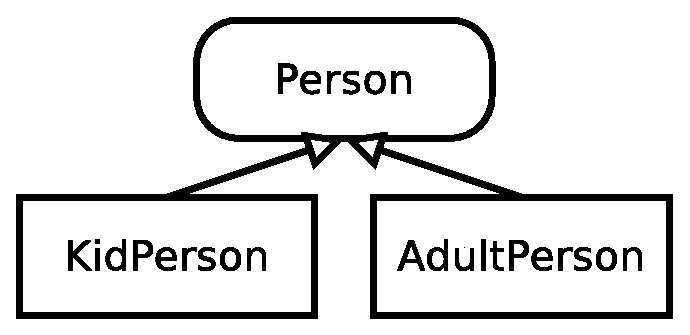
\includegraphics[height=3cm]{gfx/class_diagram-person}
  \caption{Interface Person is implemented by classes KidPerson and
    AdultPerson. By convention, the interface is represented ``up'' and
    the classes are represented ``down''.} 
  \label{fig:updown}
\end{figure}

Another useful form of upcasting is when a programmer uses an
interface as a type for a generic class: 

\begin{verbatim}
    Stack<Person> myPersonStack = new ArrayStack<Person>();
\end{verbatim}

On the left-hand side, we have a generic interface (\verb+Stack<T>+) that is made
specific by using another interface (\verb+Person+). The variable
\verb+myPersonStack+ will point to a stack that will only store
objects of classes that implement the \verb+Person+ interface
(e.g. \verb+KidPerson+, \verb+AdultPerson+, etc). 

Upcasting is a way of ``moving up to know less'', i.e.~to
intentionally forget details about the implementation so that we can
work with a simpler, more generic data type. 
Bear in mind that a real program is really complex, and therefore
reducing complexity is usually in the programmer's benefit; that
is why upcasting is so common in Java programs. 

In some rare occasions,
programmers need to do the opposite, i.e.~move down from the general
to the specific: this is called \emph{downcasting}. The syntax in this
case is very similar to the casting of simple types. Imagine that we
have a list of animals, but we knew (somehow) that all those animals
were dogs, and we wanted to make them bark. As \verb+bark()+ is a
method of \verb+Dog+ but not of \verb+Animal+ we would need to
downcast them: 

\begin{verbatim}
    public void makeThemBark(List<Animal> animals) {
        for (int i = 0; i < animals.size(); i++) {
            Animal nextAnimal = animals.get(i);
            Dog dog = (Dog) nextAnimal;
            dog.bark();
        }
    }
\end{verbatim}

Upcasting is an operation that detects errors at compile time: if the
code compiles, it will always run. This is not true of downcasting, which can
fail at \emph{runtime}, even if it compiled successfully. In the
example above, the method \verb+makeThemBark(...)+ may receive a list
of \verb+Animal+ where not all the elements are really objects of
class \verb+Dog+ (maybe there is a \verb+Cat+). When the code tries to
downcast a class into something that it is not, Java will throw a
\verb+ClassCastException+: 

\begin{verbatim}
    java.lang.ClassCastException: Cat cannot be cast to Dog
\end{verbatim}


%%% Local Variables:
%%% mode: latex
%%% TeX-master: "d12"
%%% End:

%
% \item Exercise Make a class that extends String and overwrites
%     toString() to call super.super.toString(), and then pass it to a
%     println(). 
% \item Maybe a sample test, like Roger Mitton does?(remember you
%   have a spare week (it's 11 not 10, count them JIC))... better next
%   week, so I can test up to here; plus recursion week seems a bit
%   empty.
% \item Maybe some project for groups?? -> leave for OODP
%
% ASSIGNMENT: something that uses inheritance and
%   polymorphism... great idea, now what?

% Day 13,14: Recursion!
% TODO: next year, introduce recursion before pointers? or better to
%     do it with full Java? Mmmm... given that recursion cannot be
%     graded with JUnit, it does not matter; therefore, probably
%     better to introduce it earlier, so that it can be used to work
%     with lists. -> Make sure you cover maps and trees before Xmas
%     with the part-timers (the Fenner constraint)!
%     UPDATE: early recursion means that PT go to Xmas with no
%     knowledge of generics or the Collections Library. Better to
%     leave recursion for later and remove all things recursive from
%     early days. 
%     UPDATE: major reorganisation. See above. 
% \item Recursion
% \item The execution stack (they will see it next week, if they have
%     not yet)
% \item Remember they have already seen recursion: add and delete in
%       linked lists
% \item Exercise: merge sort, quicksort (if seen after lists)
\section{Recursion}
\label{sec:recursion}

Recursion is the process of repeating items in a self-similar way. It
is a concept that appears often in computer science and other branches
of mathematics (e.g.~number theory, fractals), but it has also
attracted some interest from fields like the arts in recent times
(look up ``recursive images'' on your favourite search engine). 

In programming, the most basic form of recursion happens when a method
calls itself. This can be done in any modern programming language, and
definitely in Java. We have already seen some examples of recursive
calls, e.g.~when we tried to calculate the depth of a tree: 

\begin{verbatim}
    // Method of class Node/Tree
    public int depth() {
        int leftDepth = 0;
        if (left != null) {
            leftDepth = left.depth();
        }
        int rightDepth = 0;
        if (right != null) {
            rightDepth = right.depth();
        }
        int depthBelow = Math.max(leftDepth, rightDepth);
        return 1 + depthBelow;
    }
\end{verbatim}

This method calls itself twice before it can return a value to the
caller. In order to return the depth under a node in a binary tree,
the depth under the left branch is calculated (if it exists, otherwise
it is zero), then the depth under the right branch, and then the
result is the maximum of both depths plus one. The method
\verb+depth()+ is \emph{recursive}. 

In this section we are going to
learn more about how recursion works, when it is a good idea to use
it, and what are the possible pitfalls and how to avoid them. 

\paragraph{Classical examples: factorials and Fibonacci numbers}
\label{sec:class-exampl-fact}

The factorial of a natural number is represented with an exclamation
mark (!) and defined\footnote{If you like maths and would like to see
  how the factorial of a \emph{real} number is defined, search for the
  $\Gamma$ (gamma) function.} as:  

$$ n! = n \cdot (n - 1) \cdot (n - 2) \cdot \ldots 2 \cdot 1 $$

This definition makes it very easy to write a function that calculates
the factorial of a number recursively: 

\begin{verbatim}
    public static int factorial(int n) {
        if (n == 1) {
          return 1; 
        } else {
            int result = n * factorial(n-1);
            return result;
        }
    }
\end{verbatim}

(Note that the method is static because it has no side effects,
i.e.~it is a pure function). 

If the argument is 1, the function returns 1 (because 1! =
1). Otherwise, the function returns the argument multiplied by the
factorial of the argument minus one; that function call will in turn
return its argument (n-1) multiplied by the factorial of its argument
minus one (n-2); and so on. If we want to calculate the factorial
of~4, the resulting calculations look like this: 

$$ factorial(4) = 4 \cdot factorial(3) = 
   4 \cdot (3 \cdot factorial(2)) = 
   4 \cdot (3 \cdot (2 \cdot factorial(1))) = $$ 

$$ = 4 \cdot (3 \cdot (2 \cdot 1)) = 4 \cdot (3 \cdot 2) = 4 \cdot 6 = 24 $$

Another classical example of recursivity are Fibonacci
numbers\footnote{Fibonacci numbers were discovered by Italian mathematician
Leonardo di Pisa (known as Fibonacci) in the early 13$^{th}$ century
as an ideal solution to the growth of the population of rabbits. The
sequence of Fibonacci number starts as 1, 1, 2, 3, 5, 8, 13, 21, 34,
55, 89\ldots Fibonacci introduced arabic numerals to the West, and
thanks to him we can write 2989 instead of MMCMLXXXVIII.}.
Fibonacci numbers are defined recursively as:

$$ F(1) = F(2) = 1 $$

$$ F(n) = F(n-1) + F(n-2) $$

and have many applications in computer science and biology, among
other fields. As they are defined recursively, a recursive method to
calculate the n$^{th}$ Fibonacci number is quite straightforward to
write: 

\begin{verbatim}
    public static int fib(int n) {
        if ((n == 1) || (n == 2)) {
          return 1; 
        } else {
            int result = fib(n-1) + fib(n-2);
            return result;
        }
    }
\end{verbatim}

\subsection{How does recursion work?}
\label{sec:how-does-recursion}

Recursion works as any other method call. There is no magic. 

When a statement in Java calls a method, the same process is always
followed: 

\begin{enumerate}
\item A new level is added to the stack.
\item The values given by the caller code are copied into the
  parameters in the new level.
\item A hidden parameter ``this'' is also copied into the stack,
  pointing to the object where the method is called.
\item The code of the method is executed as usual. Any new local
  variable is created on the new level in the stack. 
\item When a \verb+return+ statement is reached, the corresponding
  return value (if any) is stored.
\item The level in the stack is wiped out, and its local variables
  (and parameter values) forgotten. The return value (if any) is
  returned to the original caller code (and usually assigned to a
  variable).
\end{enumerate}

This does not change in the case of a recursive call. If we take the
calculation of 4! before as an example, the computer stack changes are
represented if Figure~\ref{fig:fact}. First, a level is added to the
stack and the parameters are copied (only \verb+n+ in this case, with
value~4). The code of the method is executed line by line: as \verb+n+
is not 
equal to~1, a new local variable \verb+result+ is created; its value
is~1 plus the result of calling a method. A new level is added to the
stack, and the parameter values are copied (only \verb+n+ again, but
this time with value~3). A local variable \verb+result+ is created and
then the method is called again so we need to add a new level in the
stack. The process is repeated once more, and we call the method with
a value of 1 for \verb+n+. At this point, the method returns 1. Then
the calling method can finally calculate the value of \verb+result+,
which is $2 \cdot 1 = 2$, and returns it. Then the calling method can
calculate \verb+result+ itself, which in this case is $3 \cdot 2 = 6$,
and return it. The calling method can then find the value of
\verb+result+ (24) and return it. 

As you can see, a method recursively calling itself is no different
from a method calling another method. For every method call, recursive
or not, the calling code remains \emph{on pause} while the new level
in the stack is created and the code of the called method is
executed (in the example, the value is result is not defined until a
return value is received from the called method). 
When a result is returned, the calling code can continue its
execution. When a method calls a method that calls a method, etc,
several levels are added to the stack, and several methods are waiting
for a return value. Recursive calls are exactly the same, the only
difference being that the same code is executed over and over again
\emph{but on different levels of the stack}, which means that local
variables are new and independent. 

\begin{figure}[hbtp]
  \centering
  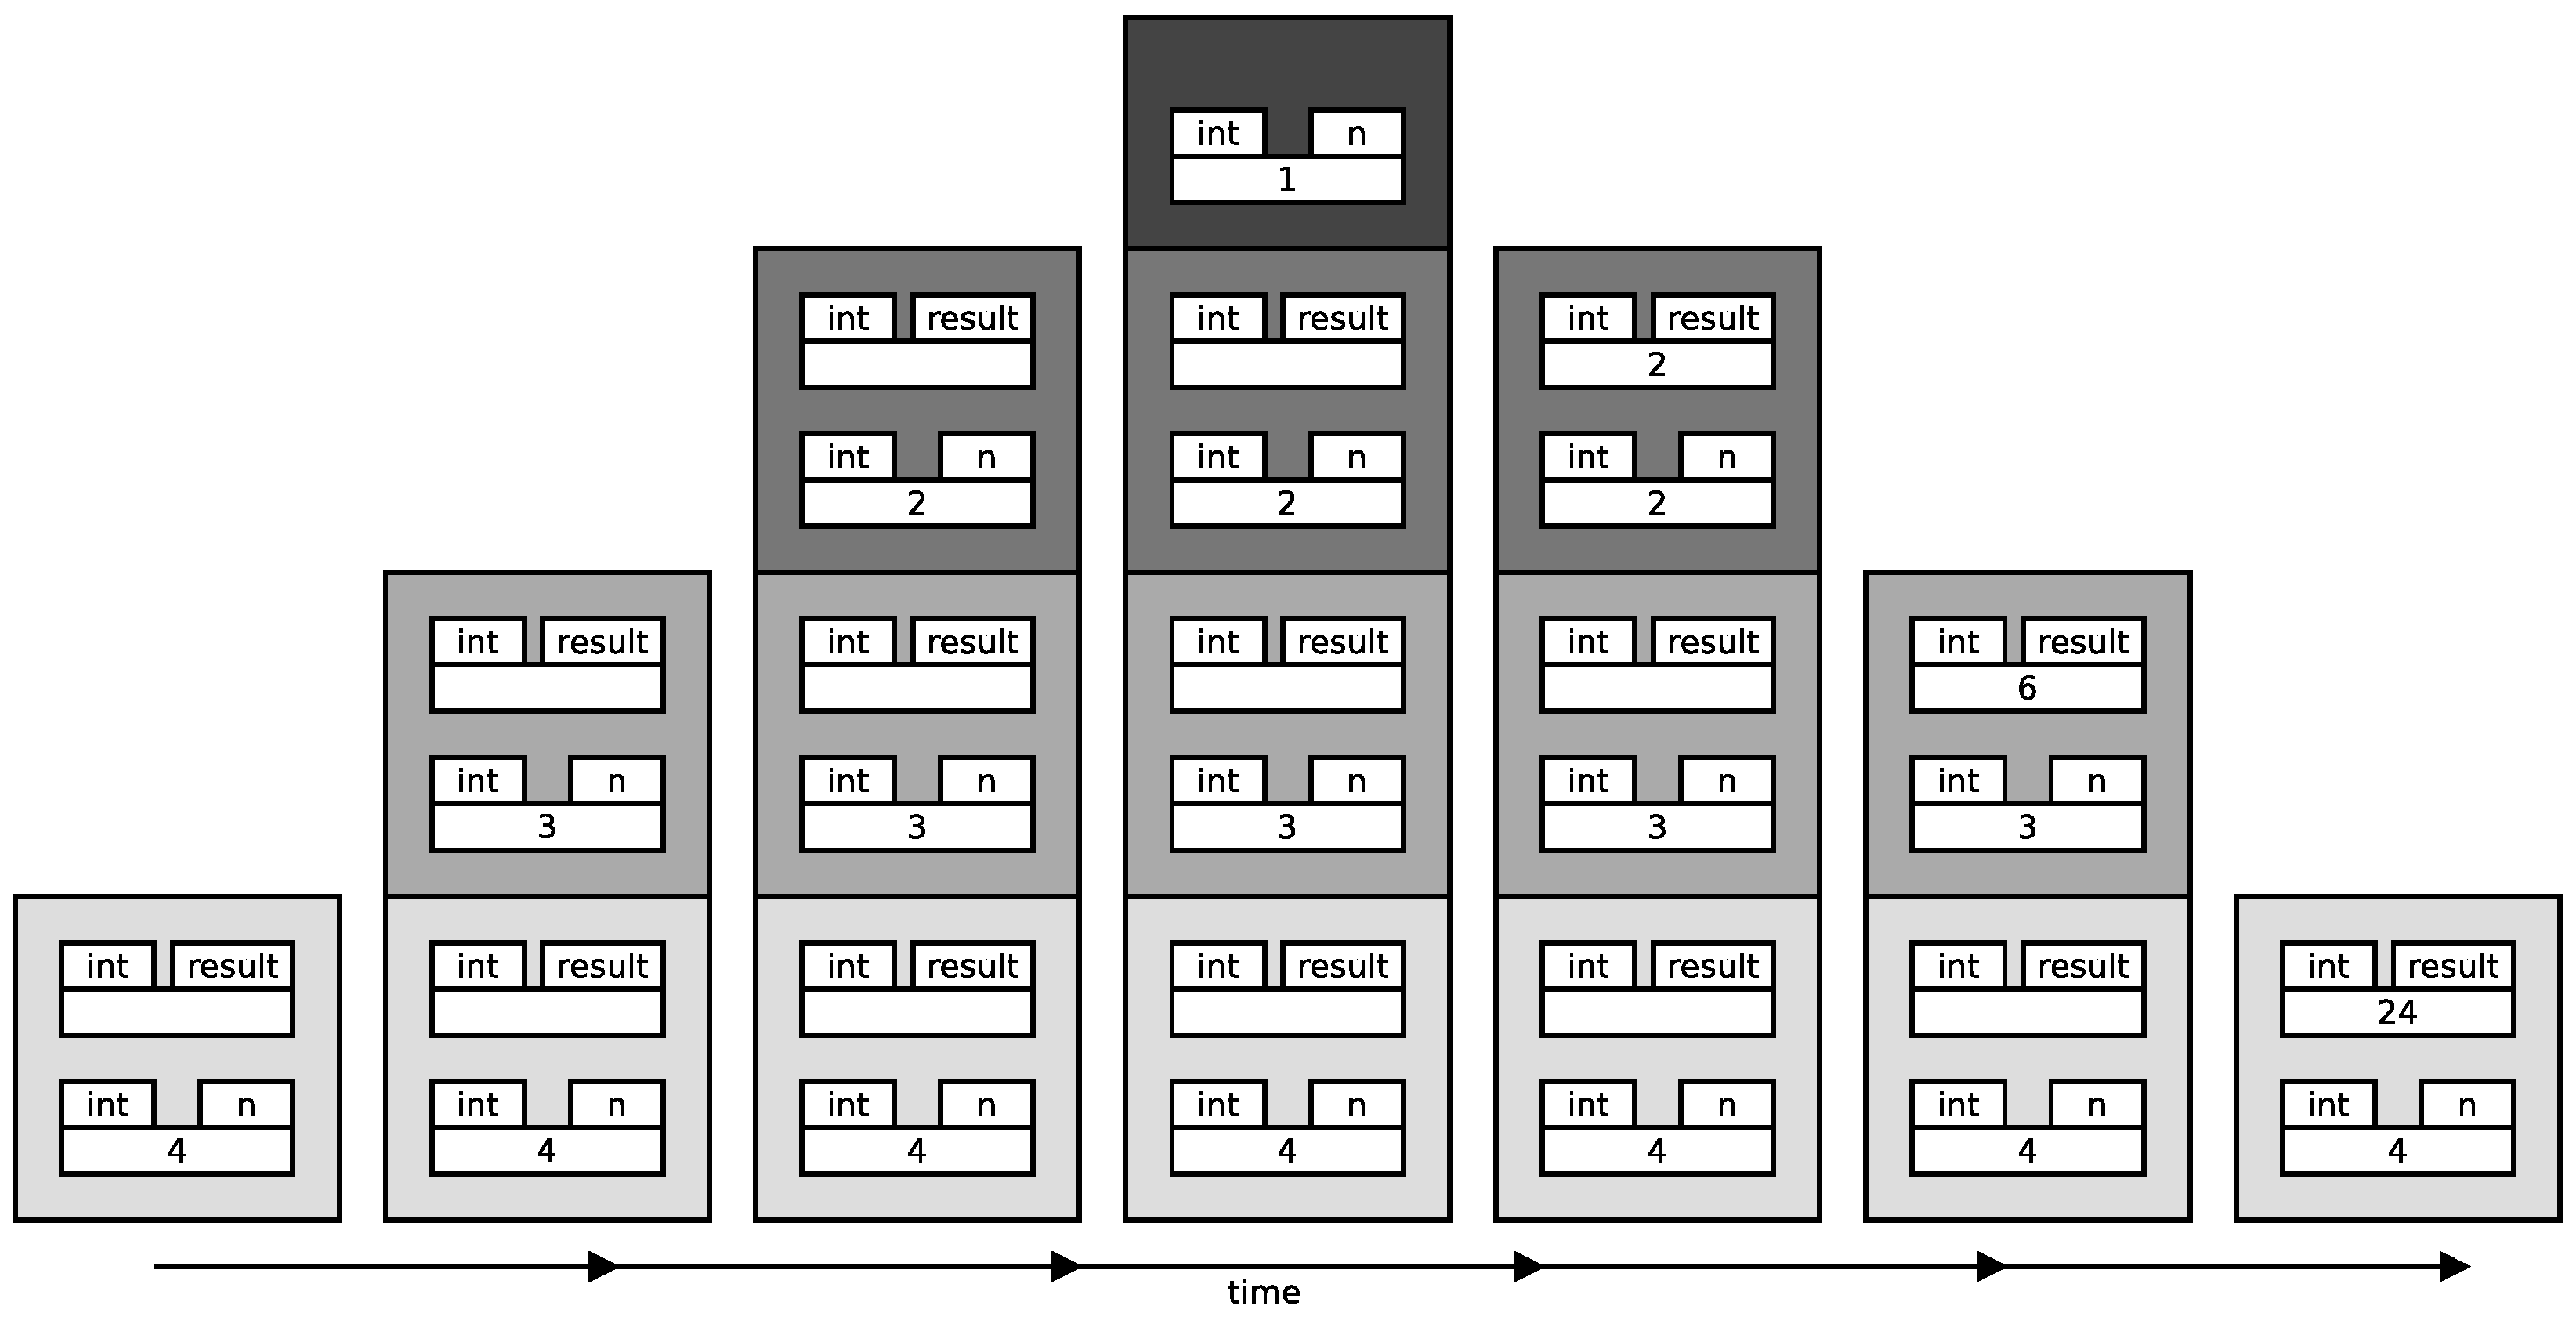
\includegraphics[width=\textwidth]{gfx/recursive-factorial}
  \caption{Evolution of the computer stack when factorial(4) is called.}
  \label{fig:fact}
\end{figure}

\subsection{Pitfalls}
\label{sec:pitfalls}

At this point you are familiar with loops (\verb+while+, \verb+for+,
\verb+do...while+) and you know that you must be careful with the
way you set the condition of a loop to prevent infinite loops that
block your programs. In a similar way, you must keep in mind a couple
of things when you write recursive code. 

\paragraph{Base case}
\label{sec:base-case}

Every recursive program or method must have a base case for which the
answer is known. In the case of the factorial, we know that~1! is~1;
in the case of the Fibonacci numbers, we know 
that the answer for F(1) and F(2) is~1; when we calculate the depth of
of a tree, we know that the depth of a tree with no descendants is 0;
when we add a new element to a a list recursively, we know that the
element will be added to the element were \verb+next+ is pointing to
\verb+null+. 

If a recursive method does not have a base case, the method will call
itself continuously until the stack is overflown, i.e.~until the
computer tries to add a new level to the stack (to execute the next
method) and find there is no more space to do it. At that point, the
Java Virtual Machine will throw a \verb+StackOverflow+ exception. 

\paragraph{No convergence}
\label{sec:no-convergence}

Apart from a base case, it is important that each iteration of a
recursive method tries to answer a simpler or more limited version of
the same question. In other words, every time a method is called again
its parameter must be a smaller number, or a shorter list, or ---in
general--- must be nearer to the base case. 

In simple cases like the factorial or the Fibonacci numbers, it is
easy to see that the method will converge. This can be more difficult
when the recursion involves more than one method, e.g.~method A calls
method B, and method B recursively calls A (A and B may be methods in
different classes\footnote{A real story: There was a project in which
  we had a window, and inside of it a canvas on which different
  objects were painted. Different elements of the application needed
  to know where the origin was; some of them asked the window and some
  of them asked the canvas. If the window did not know where the
  origin was (e.g.~at initialisation), it asked the canvas. The canvas
  set the origin at initialisation, and informed the window. If the
  user started a new canvas (e.g.~by opening a new file), the new
  canvas did not know the origin but it could as the window (which was
  already there). All was working well until the first day that a
  user, instead of starting the application and then a file, opened a
  file directly. The file opened in a canvas, that did not know where
  the origin was, so it asked the window; the window had not been told
  where the origin was, so it asked the canvas; and the recursive loop
  continued until the application crashed in front of the eyes of the
  (quite upset) user.}). You must be especially careful when you have
a loop of several methods calling each other recursively because it
may be quite complex to see whether they converge in all cases or not.

If your recursive method does not converge towards a base case, you
will overflow the stack and the Java Virtual Machine will throw a
\verb+StackOverflow+ exception. 



% Recursion
%   - takes more stack space, but usually improves legibility
%   - search for something that can only be done recursively
%     - there is no such thing, this is a consequence of the
%       Turing-Church conjecture.  
%   - when to go iterative and when to go recursive
%     - simplicity and clarity vs resources, the former win every day
%       (if they do not, they will soon)
%     - counter-example: fibonacci
%   - cpu vs memory: dynamic programming
%     - memoizing
%     - fibonacci example
%   - divide and conquer
%     - example in real life: sorting postal mail (thanks to Knuth)
%     - binary search
%     - quick sort
%     - Advantages: easier to parallelise -> will come to it again

% Exercises
%   - write numbers...  then check
%   - What is wrong with this exercise? (check for 0 is too late!)
%   - Factorial and fibonacci
%   - hanoi towers
%   - Greatest common divisor ( p > q => gcd(p,q) = gcd(q, p % q) )
%   - Anagrams of n letters
%   - adding elements / calculating length of queue
%     - Length of a queue
%   - Power of a number
%   - Koch star?
%   - Din-A4, etc
%   - merge sort
%   - Finding longest common subsequence
%   - Root finding for a polynomial (one between -1000 and 1000 if
%       sign(f(min)) != sign(f(max)) , as many as possible for **)
%   - Memoization: Collatz problem
%   - Memoization: McCarthy
%   - 8 dames on a chess board
%   - Increments and unfolding
%   - Towers of Hanoi variant: odd vs even
%   - Dominoes
%   - How big is your stack? 


%%% Local Variables:
%%% mode: latex
%%% TeX-master: "d13"
%%% End:


\section{Divide-and-conquer}
\label{sec:divide-conquer}

Some years ago, a guy called Julius Caesar conquered the Gaul in just
eight years; a remarkable feat at the time. He did not conquer the
whole Gaul in one go, but rather divided the problem (conquering the
Gaul) into smaller subproblems (conquering each small tribe) and then
solved the smaller problems to get to the final solution. 

We can use the same strategy in our programs. We can divide a problem
into smaller subproblems that we can attack more easily; once we have
the solution for the smaller subproblems, we can integrate those
solutions to get a general solution. This is called a
divide-and-conquer strategy and fits nicely with recursive
approaches. 

\subsection{More examples from the real world}
\label{sec:an-example-from}

Another example of divide-and-conquer in the real world (that, like
the Julius Caesar's example, seemed more interesting in the days before email
and twitter) is the postal mail system. The postal mail does not
deliver each letter individually, because that would be too
costly. Instead, the letter are roughly organised into zones, and then
send to the zone offices to be delivered. Zone offices do not deliver
letters individually either, but assign them to areas or postal codes,
and send them in big batches to the right local post office. The local
post office is then able to deliver all letter to their destinations. 

In the days of the internet, the Domain Name System is another example
of recursive divide-and-conquer. When you look for the server at
``www.bbk.ac.uk'', you start by asking the owner of the ``.uk''
domain. It does not have the address of every single machine in the
UK, but it knows which DNS servers are responsible of the top-level
subdomains (e.g.~co, ac, etc), so it can redirect you to the ``ac''
responsible. This server does not know every single machine in British
universities, but it know who is responsible of each subdomain
(e.g.~bbk, ox, cam, etc), and will send you to the server responsible
of ``bbk''. This server can tell you what is the address of
``www.bbk.ac.uk'' so that you can access the homepage of Birkbeck. 

As you can see, dividing the problems of postal mail delivery and
domain name resolution into smaller subproblems makes them more
manageable. You have also observed that the smaller subproblems are
basically smaller versions of the big problem. This is the type of
situation in which recursive approaches come naturally. 

\subsection{Programming example: depth and size of a tree}
\label{sec:progr-exampl-depth}

A divide-and-conquer strategy is defined by three steps: 

\begin{enumerate}
\item Division of the big problem into two or more subproblems.
\item Finding the solution of the smaller subproblems.
\item Integration of the subsolution into a solution to the big
  problem. 
\end{enumerate}

We have already seen an example of a divide-and-conquer strategy. When
we calculated the depth of a binary tree, we did not need to iterate through
all the nodes in the tree counting steps as we traversed the tree up
and down. Instead, we divided the problem into two smaller
subproblems: finding the size of the left subtree and the right
subtree. Once we found the solution of both subproblems, the
integration involved taking the maximum depth and add one to it. 

A related problem is finding the size of a tree, i.e.~the number of
elements it contains. First, we divide the problem into two smaller
subproblems: finding the size of the left and right subtrees. Once we
get the solution to those problems, we can combine them by adding them
up plus one (for the root). 



%%% Local Variables:
%%% mode: latex
%%% TeX-master: "d14"
%%% End:


% Day 15,16: Exceptions and (finally) I/O (files, mostly)
% \item Exception Handling
%   plus checked exceptions, runtime exceptions, and 
%        *never* do "catch (Exception e) {}"!
%   plus the 3 Abrahams guarantees

\section{Exception handling}
\label{sec:exception-handling}

If you try to parse as an integer something that is not an integer
number, you get a \verb+NumberFormatException+. If you try to call the
object of an object but the object is \verb+null+, you get a
\verb+NullPointerException+. But what are exceptions? And is there a
way to handle them so that they do not always crash a program? 

Exceptions represent exceptional circumstances that should never occur
in the normal (some would say \emph{ideal}) execution of a
program. When one of these exceptional circumstances ---like trying to
follow a \verb+null+ pointer--- happens, the Java Virtual Machine
throws an exception to indicate it. 

An exception interrupts the normal execution of the method where it
happened. It breaks the method where it was happening and moves up to
the calling method, where it may be caught. If it is not caught in the
calling method, it will go up again, and again, until it is caught. If
it is not caught, not even in the original \verb+main+ method, it will
be caught by the Java Virtual Machine and it will be printed on the
standard output as you have seen several times already. 

\begin{verbatim}
    Exception in thread "main" java.lang.NullPointerException
      at LinkedListNode.addNode(LinkedListNode.java:49)
      at LinkedList.addNode(LinkedList.java:30)
	at HospitalManager.launch(HospitalManager.java:71)
	at HospitalManager.main(HospitalManager.java:13)
\end{verbatim}

\subsubsection*{Reading a stack trace}

An exception contains information about the state of the Java Virtual
Machine when it was thrown. In particular, it contains the whole stack
of methods calls. This is very useful because it helps programmers to
find what went wrong (and maybe why). 

The most useful line of the stack trace is usually the first one,
because it says exactly where the exceptional situation happened. For
example, in the stack trace above we can observe that a
\verb+NullPointerException+ was thrown at line 49 of the code of class 
\verb+LinkedListNode+. With this information a programmer can look at
that specific line and try to understand why a null pointer was
accessed when this should not happen. 

If we want more information we just need to follow the stack trace
line by line. We can see that the program started at the main method
of class \verb+HospitalManager+, that the \verb+launch()+ method was
called on like 13, and that this method called the method
\verb+addNode()+ in class \verb+LinkedList+ (on line 71), which in
turn called the method \verb+addNode()+ of class \verb+LinkedListNode+
(on line 30), where the exception was thrown. 

There is no limit to the length of a stack trace. Then can have as
many steps as the size of your stack, which is several thousands of
calls deep (depending on the number of local variables per method
call). 

Sometimes the stack trace goes into code that has not been written by
us, as in the following example (comments ommitted for brevity): 

\begin{verbatim}
01    public class ExceptionThrower {
02       public static void main(String[] args) {
03          ExceptionThrower et = new ExceptionThrower();
04          et.launch();
05       }
06       private void launch() {
07          System.out.print("Write a number: ");
08          int n = getNumber();
09          String evenness = (n % 2 == 0) ? "even" : "odd";
10          System.out.println("You entered " + n + ", an " + evenness + " number."$
11       }
12       private int getNumber() {
13          String str = System.console().readLine();
14          int result = Integer.parseInt(str);
15          return result;
16       }
17    }
\end{verbatim}

If you enter numbers like 2 or 19, all will work well. However, if you
enter something like ``three'' you will get a detailed stack trace to
blame you for your incompetence typing integer numbers: 

\begin{verbatim}
    Exception in thread "main" java.lang.NumberFormatException: For input string: "three"
	at java.lang.NumberFormatException.forInputString(NumberFormatException.java:48)
	at java.lang.Integer.parseInt(Integer.java:449)
	at java.lang.Integer.parseInt(Integer.java:499)
	at ExceptionThrower.getNumber(ExceptionThrower.java:14)
	at ExceptionThrower.launch(ExceptionThrower.java:8)
	at ExceptionThrower.main(ExceptionThrower.java:4)
\end{verbatim}

We can see that the program started in the \verb+main+ method, that is called
the method \verb+launch()+, that this method called the method
\verb+getNumber()+, and then this method called
\verb+Integer.parseInt()+. From that point on, the stack trace shows
method calls happening inside classes of the basic Java Library, like
\verb+Integer+ and \verb+NumberFormatException+, but you can see that
the information is exactly the same: method calls and line numbers. If
you have access to the source code of those external classes, you will
see the line numbers and will be able to trace the stack of method
calls in detail. If you work with external libraries from which you do
not have the source code, you will only see the names of the methods
but not the line number. 

The example allows us to observer the ``interrupting'' nature of
exceptions. The \verb+NumberFormatException+ interrupted the execution
of method \verb+getNumber()+ (line 15 was not executed), then
interrupted the caller method \verb+launch()+ (lines 09--10 were never
executed), and then interrupted the \verb+main+ method. Since the
exception was never \emph{caught}, it went all the way up to the
\verb+main+ method and then was shown by the Java Virtual Machine. 

\subsection{Catching exceptions}
\label{sec:catching-exception}

Exceptions are handles by using try/catch constructs: you ``try'' some
code where exceptions may be thrown; if exceptions are thrown, you
``catch'' them and do something about them. See the following example: 

\begin{verbatim}
12    private int getNumber() {
13       int result = 0; // default
14       try { 
15          String str = System.console().readLine();
16          result = Integer.parseInt(str);
17          System.out.println("You entered " + result + ".");
18       } catch (NumberFormatException ex) {
19          System.out.println("You entered something that is not an integer number.");
20       }
21       return result;
22    }
\end{verbatim}

If a \verb+NumberFormatException+ is thrown at line 16, the normal
execution of the method is interrupted. Program execution jumps out of
the current \verb+try+ clause (i.e.~until the next closing curly
bracket). It is caught there ---there is a \verb+catch+ statement for
that type of exception---, and the code inside the \verb+catch+ clause is 
executed. Then the execution proceeds normally. 

If the exception jump up to the end of the scope and is not caught, it
will jump up to the end of the next scope. If it is still not caught,
it will jump up to the end of the next scope and so on. This usually
means that the exception is moving up the method stack from calling
method to calling method until it is caught. If it is never caught, it
will crash your program and appear on screen. 

In a way, you can think
of this as a huge \verb+catch+ statement just out of your main method
that only prints the stack trace.

\begin{verbatim}
    // WARNING: this is only a metaphore, not real code
    try {
        mainMethod();
    } catch (AnyException ex) {
        ex.printStackTrace().
        System.exit(0); // Stop the Java Virtual Machine
    }
\end{verbatim}

The method \verb+printStackTrace()+ is very useful, and is almost
always used in \verb+catch+ statements because it really helps in
debugging your program when a exception is thrown in an unexpected
place. The method prints the name of every single method that had been
called when the exception was thrown, including the line that was
being executed (if the source code for the class is known). 

A \verb+try+ clause can have many \verb+catch+ clauses associated to
it, as in the following example: 

\begin{verbatim}
12    private int getNumber() {
13       int result = 0; // default
14       try {
15           System.out.print("Enter a number with at least 3 digits: ");
16           String str = System.console().readLine();
17           result = Integer.parseInt(str);
18           System.out.println("You entered " + result + ".");
19           char thirdDigit = str.charAt(2);
20           System.out.println("The third digit is " + thirdDigit + ".");
21       } catch (NumberFormatException ex) {
22           System.out.println("ERROR 1: You entered something that is not an integer.");
23       } catch (IndexOutOfBoundsException ex) {
24           System.out.println("ERROR 2: You entered integer with less than three digits.");
25       }
26       return result;
27     }
\end{verbatim}

If a \verb+NumberFormatException+ is thrown on line~17, the execution
of the program will jump to line~21, where it will be caught. After
that \verb+catch+ clause is executed, the program will continue at the
end of the try/catch construct at line~26. If a
\verb+IndexOutOfBoundsException+ is thrown at line~19, the execution
of the program will jump to line~21, and then to line~23, where it
will be caught. After that \verb+catch+ clause is executed, the
program will continue at the end of the try/catch construct at
line~26.  
Once an exception is caught, it does not go ``up'' anymore. It
disappears. 


A \verb+try+ clause can also have a \verb+finally+ clause, which can
used for cleaning up resources. We will see more of this when we learn
about input/output. 

\subsection{Which methods throw exceptions?}
\label{sec:which-methods-throw}

The exceptions thrown by a method should be specified in the
documentation, in its JavaDoc comments. This is done by means of
\verb+@throws+. This is as important as describing the arguments for
the method or the return type. (Check the methods in the core Java
Library: they all document the exceptions they can throw). 

\begin{verbatim}
    /**
     * Gets a number as introduced by the user on the console, which
     * must be at least three digits long. Otherwise, an 
     * IndexOutOfBounds will be thrown.
     *
     * @return the number introduced by the user
     *
     * @throws NumberFormatException if the user types a not-number
     * @throws IndexOutOfBoundsException if the user types less than three digits
     */
\end{verbatim}

Additionally, many exceptions must be documented in the code
too. These are called \emph{checked exceptions}. 

\subsection{Checked and runtime exceptions}
\label{sec:check-runt-except}

All exceptions in Java extend class \verb+Exception+, in package
\verb+java.lang+. Many exceptions, including all you have met so far,
are in the same package. Classes from this package are automatically
imported, so you do not need to do import them explicitly. 

A subclass of \verb+Exception+ is \verb+RuntimeException+. Descendants
of the latter are called (unsurprisingly) \emph{runtime exceptions},
while all other descendants of \verb+Exception+ are called
\emph{checked exceptions}. The difference between these two types is
that checked exceptions \emph{must} be either explicitly declared or
explicitly caught. 

If a checked exception is thrown in some line of a method it must be
caught (by using a try/catch construct). If it is not caught, it must
be declared as (possibly) thrown up, as in the following example:

\begin{verbatim}
    /**
     * ...
     * @throws SomeCheckedException when that exceptional situation happens
     */
    public void doggyMethod() throws SomeCheckedException {
        // do things here that throw some checked exception
    }
\end{verbatim}

By declaring that the method throws \verb+SomeCheckedException+, the
programmer is telling the compiler to check that any method calling
\verb+doggyMethod+ is catching the exception\ldots or throwing it up
once again. If a checked exception can be thrown in a line, the line
must be inside a \verb+try+ block or the exception must be declared as
thrown. Otherwise, the compiler will complain. 

This does not happen with \verb+RuntimeException+. The reason is that
they are so common that it would be a lot of work to always declare
them or catch them.


\subsection{Mishandling exceptions}
\label{sec:mish-except}

There are two common mistakes when handling exceptions, and both of
them are related to laziness. As laziness is an essential part of
being human (or at least very common), it is important to be warned to
avoid the same mistakes that thousands of programmers have done in the
past (sometimes with terrible consequences). 

The first common mistake is not being specific enough when catching
exceptions. When you code throws three or four different exceptions,
it is quite tempting to use a quick \verb+catch(Exception)+ that will
work for all of them. This is usually a bad idea in the long run
because different exceptions happen in different circumstances and
should be dealt with in different ways. If you use the same code for
all of them, this may be confusing further down the line. As a rule of
thumb, it is better to catch different exceptions separately. 

The second ---and more dangerous--- mistake is not doing anything when
catching an exception. This is really bad. Once an exception is
caught, it disappears, it does not move up anymore. Unless you do
something about it, nobody will ever know that an exceptional
situation happened. For all your users know, your program may be
deleting money from their bank accounts without a hint that something
is wrong until it is too late. This is so important that I will write
it in big letter so that you do not ever forget. Repeat with me: 

\begin{center}  
{\large \bf Do not write empty \verb+catch+ blocks. Ever. }
\end{center}

Sometimes it is boring to write a \verb+catch+ block because you are
interested in the main algorithm and not the exceptional situations
along the borders of your problem. If you follow the Test Driven
Methodology we have seen in past weeks this will happen less often,
but it will happen, and you will be tempted many times to just write
an empty \verb+catch+ block and ``come later to write it
properly''. 

Believe me when I tell you that ``later'' never comes. If you cannot
think of anything reasonable for your \verb+catch+ block ---or do not
want to---, copy and paste either of the following two lines (or
both) in there and ``come later to write it properly'': 

\begin{verbatim}
    ex.printStackTrace();
    throw new RuntimeException(ex); // See more about this in next section
\end{verbatim}

If you leave empty \verb+catch+ blocks in your code you will face many
sleepless nights hunting missing exceptions and ghost bugs. You have
been warned. 

\subsection{Throwing your own exceptions}
\label{sec:throwing-your-own}

Creating your own exceptions is easy. Just create a class that extends
either \verb+Exception+ (for checked exceptions) or
\verb+RuntimeException+ (for runtime exceptions). It is rare that you
need to create additional exceptions, but in some cases it can be
useful to be more precise in your exception handling. 

Exceptions usually have three constructors: one without parameters,
one that takes a String (the message of the exception), and one that
takes another exception (so the new exception acts as a wrapper of the
old exception). 

Throwing an exception is also very easy. It is done by means of the
keyword \verb+throw+. 
(See the example below.)
Any exception can be thrown. 

\begin{verbatim}
    //...
    throw new SomeException();
    // ...
\end{verbatim}

This line creates a new exception (an object of class
\verb+RuntimeException+) and throws it. The exception can be created
in a different line, of course, and assigned to a variable. 



\paragraph{Re-throwing an exception}
\label{sec:re-throwing-an}

When an exception is caught, it disappears and does not go further up
in the method call stack. Unless we want it to happen, in which case
we can just either wrap it inside another exception and throw the
latter: 

\begin{verbatim}
    //...
    } catch(SomeException e) {
        throw new RuntimeException(e);
    }
    // ...
\end{verbatim}

or ---even simpler--- re-throw it directly (it is still an exception,
after all, so it can be thrown): 

\begin{verbatim}
    //...
    } catch(SomeException e) {
        throw e;
    }
    // ...
\end{verbatim}

The first option is quite better because it provides additional
information. I would not recommend to use the latter \emph{in any
  case}. It is only included here to illustrate the
relationship between exceptions and the \verb+throws+ keyword.

\subsection{Afterthoughts on exception handling}
\label{sec:afterth-except-handl}

\subsubsection{Should I create checked or runtime exceptions?}
\label{sec:should-i-create}

This is a difficult question, and there is not a clear answer for
it. Personally, I would recommend to make all new exceptions
\verb+RuntimeException+. 

Runtime exceptions will make your code easier to write
and not more difficult to read. They will go up your stack when thrown
and crash your program, which provides a good incentive to fix
the bug (probably by catching them at the right place). 
Not having checked and runtime exceptions (only the latter) seems
to be the route taken by more modern languages, including some very
popular ones like Python.

\subsubsection{Throw throws throwables}
\label{sec:throw-throws-throw}

The keyword \verb+throw+ can be used to throw other classes, not just
exceptions. In particular, any descendant of class \verb+Throwable+
can be thrown (and caught). 

There are two types of throwables in Java: \verb+Exception+ and
\verb+Error+. We already know exceptions. Errors are used to indicate
serious problems, like the \verb+StackOverflowError+ that is thrown
when the program runs out of stack space (e.g.~due to a buggy infinite
recursive call). It is not expected from normal applications to catch
errors, but it is possible. 

% \subsubsection{Exception handling error-checking}
% \label{sec:exception-handling-1}

% TODO: leave this section for next year



% Exercises: 
%  - Sequence flow with or without exception
%  - Read numbers. If not a number, show error message and start
%    again.



%%% Local Variables:
%%% mode: latex
%%% TeX-master: "d15"
%%% End:

% \item I/O in Java
% \item ASSIGNMENT: something that reads a CSV with rains in different
%    regions and returns a file that says who had more rains, what was
%    the average, etc

\section{Input/Output (I/O)}
\label{sec:inputoutput-io}

Computer programs are just processors of data. They take some data as
input, they return some data as output. Up to now, all the data that
our little programs have processed was either provided by a human user
or already included in the program. In the real world, however, the
most usual sources of data are computers; either the computer where
the program is running (local files), a computer in the vicinity (a
database server), or a remote computer (remote resources through the
net). 

We are going to learn now how to use the first of these three sources
of information: how to read from the local disk and how to write to
the local disk. 

\subsection{The basics}
\label{sec:basics}

\subsubsection{File systems}
\label{sec:filesystems}

Computers have different levels of memory, but there is a clear
separation between primary and secondary memory. Primary memory is
faster but requires electricity to run; if the computer is switched
on, the contents of the memory are lost. Secondary memory is slower,
but its contents are persistent, i.e.~they are still there when the
computer is switched off and on again. Seconday memory is usually
implemented in the form of a hard disk or so-called flash
memories. It is usually referred to as ``disk'', regardless of the
actual technology used for it. 

Data is stored in secondary memory in files\footnote{This name, as
  many others, comes from an ancient era where files, archives,
  directories, and folders were physical objects that contained
  documents or data.}  
The file system is a subsystem of the operating
systems that keeps all your files in place, and provides a way of
accessing them. Usually this is done by means of hierarchies: there is
one folder/directory at the top level of the hierarchy (called the
\emph{root}), which contains some files and subdirectories, each of
these subdirectories may contain files and/or subdirectories, etc. In
order to access a file \verb+taxForm2012.odt+ inside a folder
\verb+taxes+, inside a folder \verb+MyStuff+, you may access it with a
route like: 

\begin{verbatim}
    /home/john/MyStuff/taxes/taxForm2012.odt                     (unix)
    c:\Documents and Settings\john\MyStuff\taxes\taxForm2012.odt (windows)
    ./MyStuff/taxes/taxForm2012.odt
\end{verbatim}

Different operating systems use different conventions for the root of
the tree of subdirectories and the separation of the levels of
hieararchy. Unix systems (e.g.~Linux, MacOS/X) use a single root
(``/'') for the whole filesystem, and separate directories using a
slash (``/''). Windows use different roots, one per physycal device or
partition (C:, D:, etc) and separate directories with a 
backslash~(``\verb+\+''). 

File routes that start at the root are called \emph{absolute} and
those that do not are called \emph{relative} (because they point to
different files depending on the current directory). Absolute routes in
unix always start with ``/'', but in Windows they can start in
different ways (e.g.~''\verb+C:\+'', ''\verb+D:\+'', ''\verb+\+'',
etc) because there are many roots. Relative routes may start with
a dot (meaning ``current directory'') but they usually start with the
name of a file or directory. 


\subsubsection{Process}
\label{sec:process}

The process of reading from / writing to an external source always
follows the same sequence of steps:

\begin{enumerate}
\item Open the resource (e.g.~file). If it cannot be opened, finish.
\item Read from and write to the resource.
\item Close the resource. 
\end{enumerate}

This process is the basis of all interaction with external data
sources, including files, databases, and remote resources\footnote{As
  we will see, in the network resources this is usually hidden from
  the programmer.}.
It is \emph{very important to close the resource} (file, database
connection, remote connection / socket) at the
end. Otherwise, the resource may not be accessed by other programs (or
even by your same program in some situations). In a way, closing a
data source is like releasing memory that you no longer
used. Unfortunately, it is not possible to create something like a
garbage collector for data sources, so programmers have to close their
data sources manually.

\subsection{Files in Java}
\label{sec:files-java}

File names are represented in Java by the class \verb+File+ in package
\verb+java.io+. It is important to note that Java uses the unix
tradition of considering (almost) everything a file: letters and
spreadsheets are files, but so are directories for example. Therefore,
an object of class \verb+File+ can represent the name of an actual
file or the name of a directory.

This class implements a lot of methods that are useful when
interacting with the local disks. Some of the most commonly used
include: 
\verb+createNewFile()+, 
\verb+delete()+, 
\verb+exists()+, 
\verb+isDirectory()+, 
\verb+isFile()+, 
\verb+length()+, 
\verb+list()+ (lists all files in a directory), 
and
\verb+mkdir()+ (creates a directory). There are many other useful
methods, as you can see on the JavaDoc of \verb+File+\footnote{As you
  have done many times in the past weeks, you can find the JavaDoc of
  this class by searching for ``java file''. Usually the first link
  will be the documentation of the class. }, and most of them have
quite self-descriptive name. . 

Using the \verb+File+ class to get a pointer to a file (or directory)
on disk is really easy: 

\begin{verbatim}
    String filename = "filename.txt"; 
    File file = new File(filename);
\end{verbatim}

The name of the file (\verb+filename+) can be any valid route,
e.g. \verb+/home/john/file.odt+. However, there are two things that a
Java developer should keep in mind to make sure that Java programs can
run on any computer: 

\begin{description}
\item[Slash as separator] You should use slash (``/'') as a separator,
  as it works in both unix and windows systems. For extra security,
  you can use the static final field \verb+File.separator+ that always
  has the right value for the operating system the Java Virtual
  Machine is running on. Do not use names like \verb+.\myFile.txt+;
  use \verb+./myFile.txt+ instead or, to make sure it works in all
  computers:

\begin{verbatim}
    ''.'' + File.separator + ''myFile.txt''
\end{verbatim}

\item[Relative filenames: ] Your filenames should always be
  \emph{relative}, rather than absolute. Absolute routes will not work
  among different operating systems. For example, \verb+myFile.txt+ and
  \verb+./myStuff/myFile.txt+ are fine, but \verb+c:\myStuff\file.txt+
  is not. 
\end{description}

\subsection{Reading from and writing to files}
\label{sec:reading-from-writing}

Once we have a pointer to a file (through its name) we can try to open
it as we said in Section~\ref{sec:process}. Note that the file may or
may not exist. The \verb+File+ object is only a reference to the
name. If we want to know whether it exists, we can execute the
\verb+exists()+ method. 

\verb+File+ objects cannot be directly opened in Java. Instead, an
input source of data (a \verb+Reader+) can be created with a file and
it is this source that is opened (and closed at the end) to
read. Conversely, an output sink of data (a \verb+Writer+) can be
created with a file, opened, write to, and closed. 

% TODO: talk about streams?

\subsubsection{Reader}
\label{sec:reader}

\verb+Reader+ is the abstract class from which all other reader
classes descend, and it defines methods to read characters, either one
by one or many in one go. 
There are three main reader classes, each of them with
a different purpose: 

\begin{description}
\item[FileReader: ] The class for reading from text files\footnote{For
  binary files you use a FileInputStream.} (including
  common format like CSV and XML (and XML-based formats like
  OpenDocument). 
\item[BufferedReader: ] A general-purpose reader that reads characters
  from a character input stream, bufferring them for efficiency. This
  means that you do not need to read character by character. It
  provides useful methods like \verb+readLine()+.
\item[StringReader: ] A string-based reader that uses a string as the
  input source of data. Can be useful if the data is already stored in
  a String instead of being read from a file or network connection. 
\end{description}

\paragraph{Open data source}
\label{sec:open-data-source}

A \verb+Reader+ is automatically open at creation (with
\verb+new+). There is no need to explicitly open it with a method
call. 

The usual idiom to create an input source
combines a \verb+FileReader+ (to read from a
\verb+File+) with a \verb+BufferedReader+ to have access to buffered
data input and the \verb+readLine()+ method. If a \verb+FileReader+ is
directly used (without buffering), the performance of the application
may suffer. 

\begin{verbatim}
    File file = new File("here/be/the/route/to/the/file");
    BufferedReader in = new BufferedReader(new FileReader(file); 
\end{verbatim}

Creation of a \verb+FileReader+ may throw an
\verb+FileNotFoundException+, and this is a checked exception. This
means that the code above must be placed inside a \verb+try+/\verb+catch+
construct or the method must declare that it \verb+throws+ this
exception. 

\paragraph{Reading from the source}
\label{sec:reading-from-source}

Once the data source is opened, we can read from it line by line using
\verb+readLine()+. When we reach the end of the file,
\verb+readLine()+ returns \verb+null+. 


\paragraph{Closing the source}
\label{sec:closing-source}

When we have finished with reading from the file, we must close the
data source. This is easily done with the \verb+close()+ method. 

\begin{verbatim}
     in.close();
\end{verbatim}

Alert readers may have noticed that this poses a small problem. Look
at the following code: 

\begin{verbatim}
01    File file = new File("file.csv");
02    try {
03        BufferedReader in = new BufferedReader(new FileReader(file); 
04        while ((String line = in.readLine) != null) {
05            // ... do things with the data here
06        }
07        in.close();
08    } catch (IOException ex) {
09        ex.printStackTrace();
10    } catch (FileNotFoundException ex) {
11        System.out.println("File " + file + " does not exist.");
12    }    
\end{verbatim}

If a \verb+FileNotFoundException+ is thrown on line 03 nothing bad
happens; it is dealt with at the appropiate catch block. But what
happens if an \verb+IOException+ is thrown at line 04 or inside the
loop? The execution flow will jump to the catch clause on line 08,
skipping line 07 and the data source will never be closed! 

\begin{itemize}
\item We cannot move line 07 out of the \verb+try+ block because
  \verb+in+ is defined inside that scope.
\item We cannot move it to the \verb+catch+ block because that means
  \verb+in+ will not be closed if no exceptions occur, which is even
  worse. 
\item Another possibility would be to declare \verb+in+ out of the
  \verb+try+ block and initialise it inside, then closing it
  outside. However, this risks a \verb+NullPointerException+ if it is
  never initialised (e.g.~because the file does not exist or is not
  readable). 
\item Finally, a fourth possibility is to duplicate the \verb+close()+
  call, which is clearly suboptimal.
\end{itemize}

We just need a way to make sure that a data source is always closed. 

This is what \verb+finally+ is for. Every \verb+try+ can have a
\verb+finally+ block that is always executed after the \verb+try+
block; if an exception was thrown and caught, the \verb+finally+
method will be executed after the code in the \verb+catch+ block is
executed. The code would look like this: 

\begin{verbatim}
01    File file = new File("file.csv");
02    try {
03        BufferedReader in = new BufferedReader(new FileReader(file); 
04        while ((String line = in.readLine) != null) {
05            // ... do things with the data here
06        }
07    } catch (IOException ex) {
08        ex.printStackTrace();
09    } catch (FileNotFoundException ex) {
10        System.out.println("File " + file + " does not exist.");
11    } finally { 
12        in.close()
13    }
\end{verbatim}







% Talk about finally
%
% and the new way of doing finally in Java 7
% 
% Exercises: 
%
% - ls
% - cd
% - mkdir 
% - cat
% - tr
% - uniq (*)
% - sort (*)

%%% Local Variables:
%%% mode: latex
%%% TeX-master: "d16"
%%% End:


% Day 17,18: Concurrency
% Day 17:
% \item Concurrent programming
%       Thread, Runnable
%       Atomicity
%       synchronized: class and object locks 
% Day 18:
% \item package java.concurrency


% Day 19,20: Network programming (which means more I/O)
% \item OBSOLETE: Network programming: TCP, UDP
% \item Web services
% \item ASSIGNMENT: chat program

% Day 21, 22
% 
% Small mini-lecture on: how are things going to get better?
%     - No more creating your own data-structures: Java Collections Library
%     - No more modifying the classpath for JUnit -> Eclipse does it
%     - No more command-line Git (at least, not all the time)
%     - No more debugging-by-println: use the debugger
%     - Automatic indentation (and re-indentation)
%
%  - Think of a good exercise. If I take it, I will give you 5%. 



% Optional material for Day 20,21
% - Swing?
% - Reflection?
% - Regular expressions?
% - Basics of the JVM vs. other compiled languages
% - Composition over extension
% - JAR files: how to create one, how to use it from the cmd line
% - More Annotations: 
%     @SuppressWarnings
%     @Deprecated
% - Garbage collection, memory leaks, profiling... is this Tools'
%   material?
% - More of data structures: hash tables?
%  Optional (from D10):
%    Notes on optimization (use Kernigahn & Pike): 
%    - Early optimization: wrong
%    - Profiling to find *what* to optimise
%    - Techniques: 
%      - Cache or pre-computed results
%          Exercise: command-line montecarlo simulator: parse
%              expressions and execute, with and without cache
%


\appendix

\chapter{Obtaining, installing and running Groovy on a PC}
\label{sec:obta-inst-runn}
 
You can download a free copy of the Groovy compiler and runtime environment 
from the web:

\begin{verbatim}
    http://groovy.codehaus.org/Download
\end{verbatim}

Groovy can run on any computer with Java installed, including the main
operating systems like Windows, Linux, and Mac. If you do not have
Java installed in your computer, you can install it from the web:

\begin{verbatim}
    http://www.java.com/en/download/index.jsp
\end{verbatim}

Java will be used intensively in several of the MSc courses 
at Birkbeck, so it is a good idea to install it if you do not have it
yet.

If you do not know whether you have Java or Groovy installed in your
system, you can open a command prompt\footnote{You can find it in Windows in
  ``Accesories''} and type\footnote{In some systems, you can type
  ``-v'' instead of ``-version''.} \verb+java -version+ 
or \verb+groovy -version+. 

If they are installed, the result should be something similar to this:

\begin{verbatim}
    > java -version
    java version "1.6.0_23"
    OpenJDK Runtime Environment (IcedTea6 1.11pre) (6b23~pre11-0ubuntu1.11.10.1)
    OpenJDK Server VM (build 20.0-b11, mixed mode)

    > groovy -version
    Groovy Version: 1.7.10 JVM: 1.6.0_23
\end{verbatim}



\subsection*{Compiling and running Groovy programs}

The Groovy compiler is run from the command line.

You first type your program in a text editor. Notepad (in Windows) or
gedit (in Linux) are good options, but any simple editor will
do. Note: If you use a word-processor (like Microsoft Word or
LibreOffice Writer), make sure you save the file as text.

Give the filename a \texttt{.groovy} extension.

Open the command prompt. 
Go to the folder where you have saved your Groovy
program using the command ``cd'' (change directory). (You do not have to
do this but it is easier if you do, otherwise you would have to type the full
path for your source code file to compile it.)

Suppose your program is in a file called 
\texttt{Myprog.groovy} in the current folder. 
You can compile and run your program in one step by typing 

\begin{Verbatim}
    groovy  Myprog.groovy
\end{Verbatim}

If the compilation is successful, you will see the result of your
program on the screen.
%
If there are compilation errors, you will get error messages and you need
to go back to the text editor, correct the program and save it again,
then recompile it. 



\subsection*{If you cannot install Groovy\ldots}
\label{sec:if-you-cannot}

If you have problems installing Groovy, you may find this webpage useful:

\begin{verbatim}
   http://www.tutorialspoint.com/execute_groovy_online.php
\end{verbatim}

The page provides you with an editor at the top and a console at the
bottom. It will allow you to test your programs online. It is quite
slow compared to using a local machine, but it may help if you find
problems installing Groovy. 

Additionally, if you have any problem installing or running Groovy,
feel free to write to Dr. Sergio Gutierrez-Santos
(sergut@dcs.bbk.ac.uk). We will come back to you as soon as possible.

%%% Local Variables:
%%% TeX-master: "primer"
%%% End:



\chapter{Source code version control}
\label{sec:source-code-version}
%TODO: stress the point of initialising a REPO, not just I: or H:


\section{Version control}
\label{sec:version-control}

What is version control? It is something as simple (and as difficult
to make right) as keeping track of changes in some piece of work, over
time. You
are probably familar with some very rudimentary version of version
control. Have you ever listed the documents in a folder and seen
something similar to this?

\begin{itemize}
\item myDocument
\item myDocument-2
\item myDocument-3
\item myDocument-final
\item myDocument-final2
\item myDocument-final-final
\item myDocument-definitive
\item myDocument-defitive-USE-THIS-ONE
\end{itemize}

If so, you already understand the most important idea behind version
control: our work is never created in one go, it changes over time and
sometimes we want to make sure we can go back in time to a former
version of it\ldots just in case. 

Many modern programs have version control embedded into them,
e.g. word processors like Microsoft Word, OpenOffice Write, or Google
Docs (also known as Google Drive). Very often they just track the
changes made to the document, sometimes they allow the user to go back
and forth in time to review, accept, or discard changes. This is also
very common in wiki sites like the Wikipedia. 

% TODO: add a screenshot of the version control in wikipedia here. 

Version control systems were initially created to track changes in
\emph{source code}. They were created by programmers for
programmers. We have come a long way since those days, and now version
control is spread over many different applications, but they still
pursue the same two goals: 

\begin{description}
\item[Reversibility: ] the capacity of going back in time if you mess
  up and introduce bugs in your code (sorry, I meant \emph{when} you
  introduce bugs in your code).
\item[Concurrency: ] the capacity of working together with other
  people on the same project, on the same file, at the same time. 
\end{description}

These two capacities are basic for any modern programmer, and that is
why version control is (or should be) part of every programmer's daily
life. Modern programs are big and complex, and several programmers
work on them. Without appropriate version control, they cannot work at
the same time: they need to take turns, pass the baton\ldots this is
really unproductive, good programmers do not work like
that. Additionally, programmers ---even good programmers, as long as
they are human--- make mistakes all the time, sometimes serious
mistakes that break their programs completely, and they need to go
back in time to the point where everything was working fine and start
again (in large and complicated programs, this may mean a long time).

In this chapter we will learn to make version control on your source
code files \emph{right}, not as shown above (e.g. myProgramOLD.jdc,
etc). We will use a program for doing so called \emph{Git}.

\section{Git}
\label{sec:git}

There are many programs for performing source code version control
nowadays. For this course, we are using Git, a version control system
created by Linus Torvalds, the same guy that created Linux. It is not
difficult to use but it is very powerful. 

Other very common version control systems are Subversion (also known
as svn) and Mercurial. There are many more. There are many sources
online, starting with Wikipedia, that will tell you the history of
version control, the differences between different systems, and much
more. I encourage you to go and read about it if you think the topic
is fascinating. If you just want to learn to use Git normally in
your life as a programmer, this section will help you learn the
basics. 

As you can imagine, a full book could be written about all the
possibilities and options that come with Git ---actually, several ones
have been published already. In this section I will just present the
most important 10\% of Git, which is all 
you will need 90\% of the time.  

\subsection{Starting a new project}
\label{sec:starting-new-project}

Let's start by creating a new programming project. There are two ways
of doing this, locally and using an online repository manager. As the
latter is simpler from the point of view of sharing your code (more on
that later), we will explain that option here. 

We will use GitHub (www.github.com), 
one of the most well-knowned online repository
managers\footnote{There are many others: BitBucket, Google Code\ldots
  the list is endless.}. 
It is also costless to use, which is a big plus. 

\begin{figure}[htbp]
  \centering
  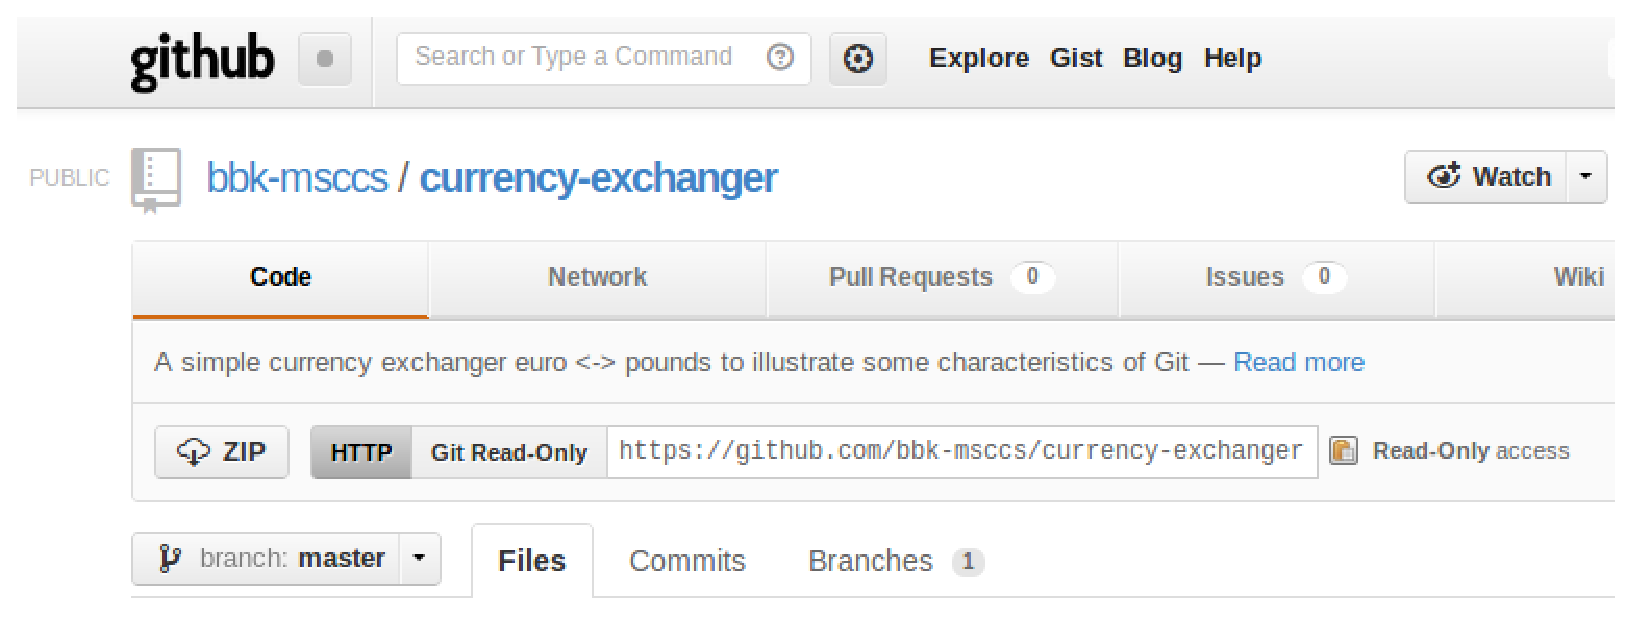
\includegraphics[width=\textwidth]{gfx/gitHubScreenshot.eps}
  \caption{Screenshot of GitHub. You can see the name of the user
    (``bbk-msccs''), the name of the repository
    (``currency-exchanger''), and the URL. 
    % You can use the URL both to
    % clone the reposity and to push your changes (as long as this
    % repository is yours, i.e. you can \emph{write} on it).
    }
  \label{fig:github}
\end{figure}

Creating an account on GitHub is easy and free. Click on the ``Create
a repo'' button, choose a name and a description, and you are ready to
go. It could not be easier. 

Now that you now how to create repositories, we will learn how use
them to keep track of the evolution of your source code. For the
purposes of the following discussion, I will assume that you have an
account at GitHub and that your account name is ``ilovegit''.  In some
cases I will need a sample repository to explain some of the features;
unless the text says otherwise, I will assume that you have created a
repository in GitHub called ``my-currency-exchange'' and the examples
will refer to this repository created by ``ilovegit''.

% REMOVED - FOR EXTRA INFO

% Create a new folder
% where you will put your programs. Now we want to start keeping track
% of all changes. Assuming Git is installed in your system, and that you
% are on the right folder, you only need to type \verb+git init+. With
% this simple command, you have told Git to \emph{be ready} to keep 
% track of whatever happens in this folder. So the full initialisation
% of a complex complete version control system with Git looks like this: 

% \begin{verbatim}
%     > mkdir MyProject
%     > cd MyProject
%     > git init
% \end{verbatim}

% That was easy, wasn't it? Now you can keep track of all changes to
% your files in this folder. Moving on\ldots

% \subsection{Name and email address}
% \label{sec:name-email-address}

% Every time somebody makes a change to a program, Git marks the change
% with the name and the email address of the person responsible for it. 
% As you do not want to do is writing your
% name and your email address every time you make a change, this is
% usually set up at the beginning. You can do it with the command 
% \verb+git config+. 

% \begin{verbatim}
%     > git config --global user.name "John Smith"
%     > git config --global user.email "john.smith@student-bbk-ac-uk"
%     > git config --global user.email "john.smith@gmail"
% \end{verbatim}

% These commands will set your name and email address for every (local)
% repository in your machine because you are using the \verb+--global+
% flag. 
% %
% Without the \verb+--global+ flag, 
% the command modifies the configuration of
% the current repository only. 
% Sometimes you want to have different names or
% emails on different repositories, although this is rare. 

% Note that the email address does not need to be valid. To avoid spam,
% it is not uncommon for users to use email addresses that are perfectly
% understandable for human beings but confusing for spambots, 
% e.g. removing the last \verb+.com+ (john.smith@gmail)
% or changing dots for dashes (john.smith@student-bbk-ac-uk).

\subsection{Think global, act local}
\label{sec:cloning-technology}

A repository is just a place (somewhere on the internet or in a
private intranet) where the source code for a software project is
stored. There are two types of repositories for any project:
\emph{local copies}, where you do the work; and \emph{one public
  copy}, that other people can look at.  Any machine on the internet
can be used to host a public copy of a Git project and GitHub
(\verb+www.github.com+) is a convenient place that many people use.

You cannot write your programs on GitHub, you can only do it in your
local copy. Therefore, the first thing you have to do after creating
your repository on GitHub is making a local copy, a process known as
\emph{cloning}. 

\begin{verbatim}
    > git clone https://github.com/bbk-myName/my-repository.git
\end{verbatim}

This will create a local copy of the remote repository you have just
created. You can now make changes to it: create new files, modify the
existing ones, etc.

(You can also clone repositories that were created long time ago and/or
by other people. More on that later.) 

\subsection{Keeping track of changes}
\label{sec:keep-track-chang}

Let's start by writing some code. For example, let's create a
simple \emph{Hello World} application in Groovy\footnote{Feel free to
  use Java Decaf or Java instead of Groovy for the following
  examples.}. In other words, we 
will edit a file called \verb+helloworld.groovy+ and write on it:

\begin{verbatim}
    print "Hello World!"
\end{verbatim}

If we execute this little program, it will print the words ``Hello
World!'' on the screen. So far, so good. Time to start filling up our
\emph{version journal}! 

The first step is to tell Git that we want to keep track of this
file. In other words, we \emph{add} it to the list of files under
Git's responsibility. 

\begin{verbatim}
    > git add helloworld.groovy
\end{verbatim}

And now we must perform the most important operation in any version control
system: \emph{committing} our changes. 

\begin{verbatim}
    > git commit
\end{verbatim}

You will be asked to introduce some description of what this \emph{commit}
is about. Git automatically adds information about which files are
committed and what changes have been performed on them. The programmer
must provide some additional information: a short message to explain
to other programmers what the changes are about. Note that ``other
programmers'' can mean yourself in two weeks time ---when you have
forgotten what you committed at this point. Typical messages are
``First commit'', ``Fixed bug \#1304'', ``Added a new feature
for\ldots''; examples of bad non-informative commit messages are ``new
commit'', ``More code'', or ``Fixed it AT LAST!'' (what is
\emph{it}?). Write whatever you 
want, but make a (small) effort to think what message will be useful
for people reading it in the future.

When you finish writing your commit description, save it and close the
editor. The commit will be performed, and you will be given some
output from Git. That output will include information about the
branch (by default, it is called \emph{master}), the identifier for
this commit (a unique identifier similar to ``12a0006''), 
your commit text, and some 
statistics about what the commit did: lines added, edited, or removed,
files added or removed, etc (\emph{see
  Figure~\ref{fig:git-example-output}}). 

\begin{figure}[htbp!]
  \centering
  \begin{framed}
    \begin{verbatim}
   > git commit
   [master 12a0006] Added first line: just says "Hello World!"
   1 file changed, 7 insertions(+), 1 deletion(-)
   >
   \end{verbatim}
  \end{framed}
  \caption{Example of Git's output after a commit.}
  \label{fig:git-example-output}
  % TODO: add hand-written tags to screenshot
\end{figure}

Now your project has a history! 
It looks more or less like Figure~\ref{fig:git-example-1}.
Not very impressive, but we are just starting.

\begin{figure}[htbp!]
  \centering
  \includegraphics[width=\textwidth]{gfx/commit_history_1.eps}
  \caption{Initial history of this project}
  \label{fig:git-example-1}
\end{figure}


\subsubsection*{What to do when you mess up}
\label{sec:what-do-when}

Let's say we are not happy with our program. It does not do much. We
can modify the program to look like this:

\begin{verbatim}
    println "Hello World!"
    println "What's your name?"
    String s = System.console().readline()
    println "Hello " + s + "!"
\end{verbatim}

Once we have saved the changes, we can commit again (\verb+git add
helloworld.groovy+; \verb+git commit+, plus a commit description). 

However, if we try to run the program, Groovy will complain. 
We have messed up! At this point, we have two options:

\begin{itemize}
\item If we know where the problem is (and in this simple example, we
  do) we can just fix it and commit again. A good commit message would
  be ``Fixed typo in line 3: readline() should be readLine()''. The
  history of the project is represented in
  Figure~\ref{fig:git-example-2}. 
\item If we did not know where the problem is, as it is usually the
  case in big programs, we can go back in time
  until we find the commit in
  which the problem started. Looking at the changes on that commit we
  can see how the \emph{bug} was introduced. Thanks to version
  control, finding bugs is much easier (and 
  finding bugs is 80\% of the job). 
\end{itemize}

\begin{figure}[htbp!]
  \centering
  \includegraphics[width=\textwidth]{gfx/commit_history_2.eps}
  \caption{History of this project after second commit}
  \label{fig:git-example-2}
\end{figure}

The simplest way to travel in time is by looking at the change log of
a file, and we are going to see how to do that in the next section. 

\subsection{Looking into the past}
\label{sec:looking-into-past}

Contrary to most novelists, professional programmers do not usually
start working on a project from a blank editor page. 
The most common situation is to work
on a project that has already been going on for some time. Maybe the
programmer is a new employee in the company, or has been transferred
to a different project, or has ``inherited'' a project that somebody
else started. Or it may be that the programmer wants to contribute to
another project because the project is appealing or
famous\footnote{Examples of interesting free/open-source projects with
  many contributors include web browsers like Firefox or Chrome, the
  Linux kernel, the Android operating system (based on Linux), the
  LibreOffice suite of applications, mail programs 
  like Thunderbird, and many others.}. Or maybe the programmer starts a
project from scratch and then realises that somebody else is doing the
same thing, only they started long ago and have made a lot of
progress, so it makes sense to join their team instead of reinventing
the wheel. For any of these reasons ---and many others--- you will
find yourself in a situation where you want to get a copy of the
source code that other people have written. This is very easy to do in
Git. You just need to be given a URL\footnote{A Uniform
  Resource Locator (URL) is a specific character string that
  constitutes a reference to an Internet resource. Examples of URLs
  are \texttt{http://www.bbk.ac.uk} and
  \texttt{ftp://gb.archive.ubuntu.com/ubuntu/}.
} to the source code, and clone it. Cloning other people's project
works in the same way as cloning your own project: 

\begin{verbatim}
    > git clone https://github.com/bbk-msccs/currency-exchanger.git
\end{verbatim}

Now that we have a copy of the Currency Exchanger project, let's look
at it. You will see that it has only two files: a ``read me'' file
called \verb+README.md+ (that explains what the project is about) and
a Groovy file called \verb+currencyConverter.groovy+. This is the
interesting one. 

Look at the code of \verb+currencyConverter.groovy+ and understand
what it does and how it works. Then come back and continue reading. Go
on, I will wait for you here. 

As you can imagine, this little program was not written in one go. You
can see a summary of the history of the file by looking at its
\emph{commit log}: 

\begin{verbatim}
    > git log currencyConverter.groovy
\end{verbatim}

This will show the list of commits on your screen, ordered
chronologically. For every commit, you can see the commit ID, the
author, and the date and time on which the commit was made. You can
also read the commit message. 

You can pass arguments to \verb+git log+ so that Git only shows you
commits for one author, or between two specific dates, and many
other options. Type \verb+git help log+ for more information. You can
use \verb+git help <command>+ to get help on any other command. 

The problem with \verb+git log+ is that it does not show how the code
changed from one commit to the next. But there is a way to do this:
\verb+git diff+. Let's have a look at an example: 

\begin{verbatim}
    > git diff ab9d6 9ecf9
\end{verbatim}

This command shows the changes between those two commits. Note that I
did not have to write the whole commit ID (40 characters!) but only
the first five are fine \emph{as long as they are unique}. If the
shortened IDs you use are not unique, Git will complain. In this case,
the short IDs are unique and Git tells that only one line was changed: 

\begin{verbatim}
    index 2d97cf4..5650842 100644
    --- a/currencyConverter.groovy
    +++ b/currencyConverter.groovy
    @@ -23,7 +23,7 @@ while (!finished) {
        case 2: 
            print "How many euro would you like to convert? ";
            double euro   = Double.parseDouble(System.console().readLine());
    -       double pounds = euro * poundOverEuroRatio;
    +       double pounds = pounds * euroOverPoundRatio;
            println euro + "€ will give you £" + pounds;
            break;
         case 0:  
\end{verbatim}

The ``-'' sign on the margin shows a deleted line while the ``+'' sign
shows an added line; the other lines were not changed. 
If you take everything into account, the only thing that changed
in this commit was the name of two variables on that line. 

You can also use some special tag names for referring to a commit, as
shown on Figure

\begin{table}[hbtp]
  \centering
  \begin{tabular}{p{2cm}p{8cm}}
    ID & Identifies\ldots \\
    \hline
    9ecf9 & \ldots any commit as long as the string is unique \\
    HEAD & \ldots the latest commit done \\
    ^ & \ldots this suffix identifies the commit before another one \\ 
    HEAD^ & the commit before the latest \ldots \\
    9ecf9^^ & \ldots the commit before the commit before \emph{9ecf9} \\
  \end{tabular}
  \caption{Commit names in Git}
  \label{tab:tagnames}
\end{table}

\subsection{Sharing is caring}
\label{sec:sharing-caring}

\subsubsection{Push}
\label{sec:push}

If you wanted to improve this program, you could edit it yourself, add
new features, change some code, etc. You would commit regularly to
make sure you always have the history of your project up to date, so
you can see what changes you introduced over time. 

At some point you will want to make your changes public (in Git
jargon, this is called \emph{pushing your changes}), e.g. to allow
other members of your team to see what you have done. To make your
changes public, you usually need a place to put your \emph{public
repository} (as opposed to your \emph{local copy}, where you
work). You can host your public repository anywhere you want, but
GitHub is a convenient, well-known, and costless possibility. For the
purposes of this discussion, I will assume that you have an account at
GitHub, that your account name is ``ilovegit'', and that you have
created a repository in GitHub called ``my-currency-exchange''. 

% The first thing you have to do (but you only need to do this the first
% time) is telling Git where to push the changes. This is done by adding
% a remote site (with the command\ldots \verb+git remote+, surprise!):

% \begin{verbatim}
%     > git remote add origin https://github.com/sergutsan/groovyck.git
% \end{verbatim}

% There are many things on that line that need explaining. First,
% ``add'' tells git that you want to add a new remote site; you can also
% remove (``rm'') and rename (``rename'') remote sites. By default,
% \verb+git remote+ will just show a list of your remote sites (name,
% url\ldots). The word ``origin'' is just a name for the new remote site
% to be used locally; origin is a common name for the main repository
% where you push your changes. We could have used ``my-projects'', or
% ``myRemoteSite'', or any other name as long as we have not used it
% yet. Finally, the URL is where the remote site
% is. GitHub\footnote{GitHub does give you much more than just hosting
%   your repositories: issue tracker, statistics, graphs, and limited
%   social networking capabilities are some of the features you can use
%   easily from their webpage. Not bad for a free service. Another good
%   option is Google Code.} will give
% you a URL that you can copy and paste (see Figure~\ref{fig:github}).

% \begin{figure}[htbp]
%   \centering
%   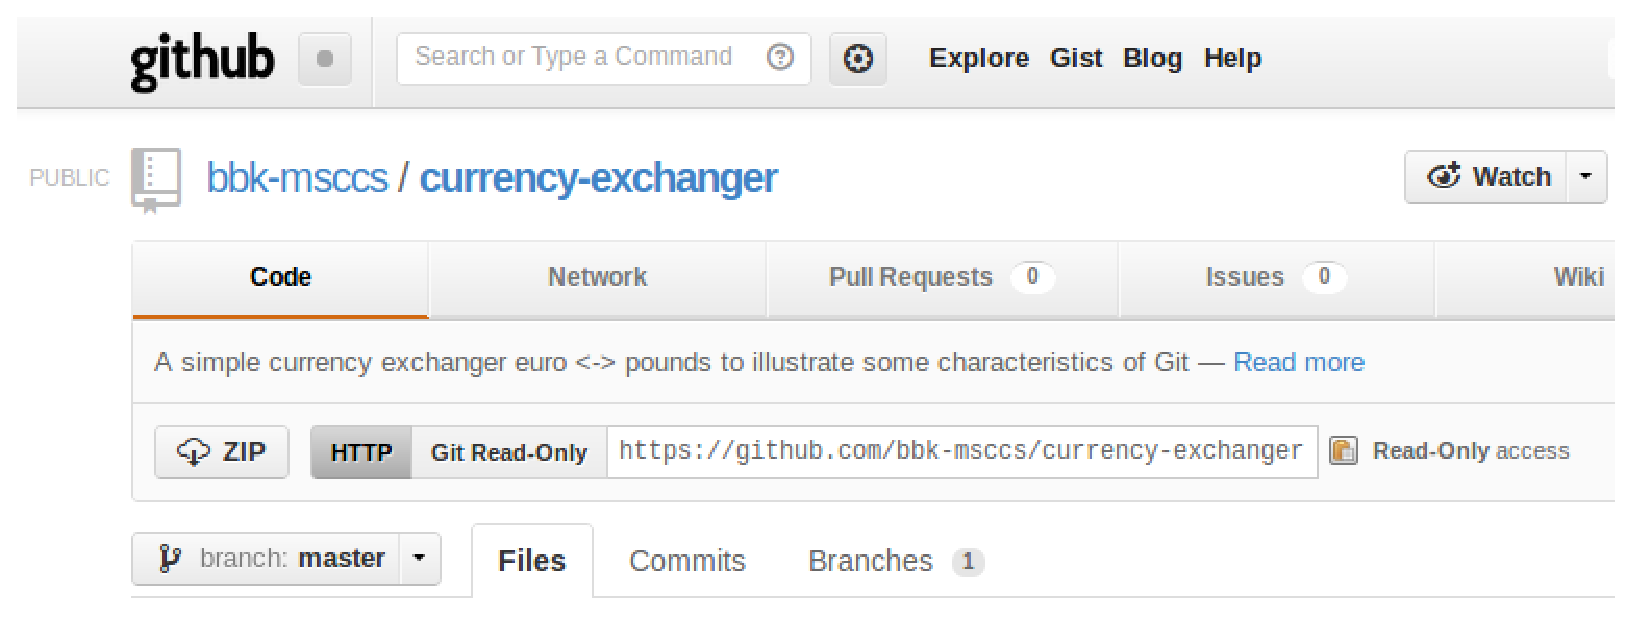
\includegraphics[width=\textwidth]{gfx/gitHubScreenshot.eps}
%   \caption{Screenshot of GitHub. You can see the name of the user
%     (``bbk-msccs''), the name of the repository
%     (``currency-exchanger''), and the URL. You can use the URL both to
%     clone the reposity and to push your changes (as long as this
%     repository is yours, i.e. you can \emph{write} on it).}
%   \label{fig:github}
% \end{figure}

% Once you have configured your remote repository or repositories,
% pushing your changes is very easy: you only need to say where to push. 

\begin{verbatim}
    > git push origin 
    Username for 'https://github.com': ilovegit
    Password for 'https://ilovegit@github.com':
    To https://github.com/ilovegit/my-currency-exchange.git
    6457568..55ca3da  master -> master
\end{verbatim}

The system will ask for your username (``ilovegit'' in this example)
and your password. Then, if everything goes according to plan, 
it will inform you that it has pushed your commits. Note that 
this step could
fail for several reasons, like your network connection going down. 

\subsubsection{Pull}
\label{sec:pull}

Once you have pushed your changes, how do other people see them? How
do they take the code you have \emph{pushed} into your remote
repository and put in their local copies of the source code? As you
can imagine, they \emph{pull} it. 

\begin{verbatim}
    > git pull origin master
\end{verbatim}

When you pull, you have to specify the remote repository you are
pulling from (``origin'' in this case) and the branch you are pulling
from. We will talk later about branches, but for now it suffices to
say that the default branch in most projects is called ``master'', and
sometimes it is the only one. If you are not sure which branch you are
pulling from, ``master'' is usually a good guess.

Once you pull, Git will download the changes made public at that
public repository and merge them with your local copy. At this point,
you have the latest copy of the project's source code, including those
changes that somebody else (maybe you) made in a different computer. 

At this point, you have surely noticed that Git can be used to
synchronise with other team members, each other pulling whatever
changes others have pushed so that everybody is up to date; but it can
also be used to keep up to date with yourself: you can work on
different computers (at home, at the office, on your laptop on a
plane) and you can push your changes and then pull them from the other
computers. There is no need to carry around USB sticks with folders
called ``currencyExchangev2'', ``currencyExchangev3'', or
``currencyExchangev4usethisnottheother''. Git will always have the
latest version as long as you do not forget to commit and push
timely (Figure~\ref{fig:pushpull}). 

\begin{figure}[htbp!]
  \centering
  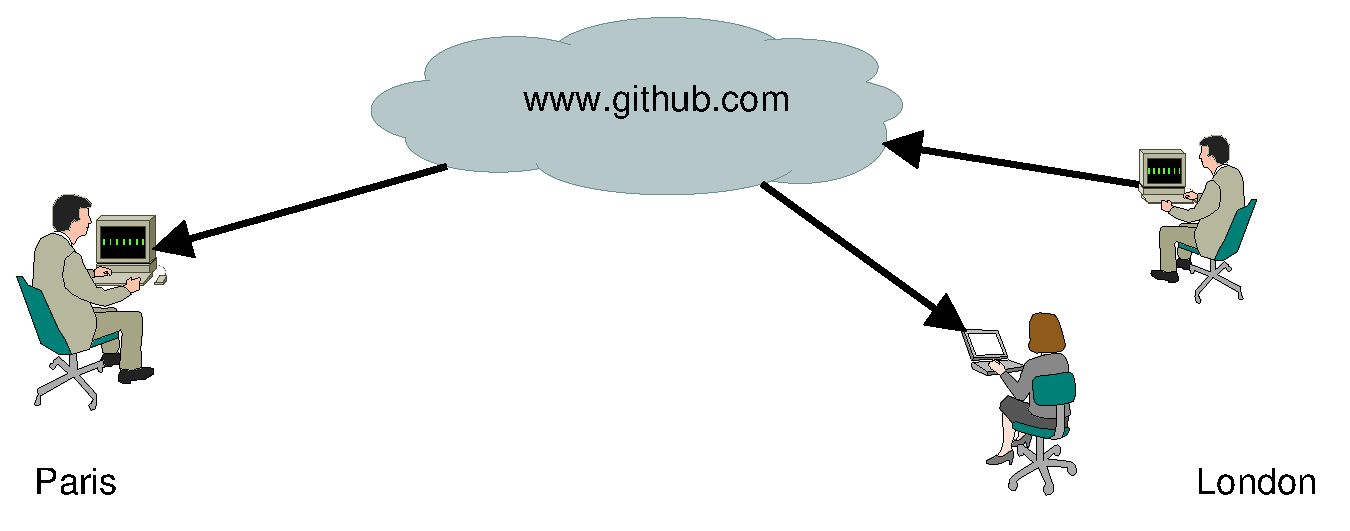
\includegraphics[width=\textwidth]{gfx/pushpull}
  \caption{Pushing and pulling: when Alfred pushes his changes to make
    them public, Bertha will be able to pull them and work on the last
    version of the software. If Alfred takes a plane to Paris, he will
    be able to pull the changes from Paris to get the last
    version\ldots including any changes that Bertha and other
    co-workers may have pushed while he was on the plane!}
  \label{fig:pushpull}
\end{figure}

\subsection{When should I commit?}
\label{sec:when-should-i}

As a general rule: \emph{commit early, commit often}. It is generally
a good idea to make small commits so that it is easier to go through
the history of your code and understand every step if you have to. The
cost of 
committing is almost zero so you should not be afraid of having too
many commits. There is no such thing. 

Of course, this does not mean that you commit every single character
that you write. Committing every single line is also probably too
much, unless those lines are really special (e.g.~they fix a bug). 
\emph{Do not spend more time
writing commit messages than writing code}. That said, if you have not
committed for the last half hour, either you have written a lot of
code and you should commit early (as in \emph{now}); or you are tired
or distracted, and not really programming, so maybe you should have a
break.

If you are not sure what you have changed since the last commit, 
you can use \verb+git diff+. Another ---less verbose--- possibility
is to use \verb+git status+. The latter will tell you
which files have changed since the last commit, without details of the
changes.

Additionally, you should \emph{push} your changes to your public
repository fairly often. Some people say \emph{push early, push
  often}, but it does not mean that you need to push after every
commit. Sometimes 
you cannot even push because you do not have a network connection,
although this is becoming more and more uncommon these days, where you
can connect to the internet from planes, submarines, and almost a
robot wandering around Mars\footnote{Actually, a robot in Mars cannot
  connect to the internet, at least not what we call ``the Internet'' 
  in 2012 (computers interconnected using the TCP/IP and related protocols). 
  Radio waves travel \emph{only} as fast as light-speed, and it
  takes them so long to reach the Earth that internet hosts would
  timeout before a connection could be stablished. 
  You \emph{could} connect to
  the Internet from the Moon, though, but your bandwitdh would be
  very poor compared to your home connection.}. 
As a rule of thumb, push every time you 
have finished a coding session (e.g. before turning off the computer
or standing up to grab some lunch), or as soon as possible after that.

\subsection{Back to the past\ldots}
\label{sec:branching}

If you have been reading carefully until now, you will have noticed
that we do not know yet how to \emph{move back in time}. So far we
have only learnt how to look into the past using \verb+git log+. In
order to be able to \emph{roll back} when we mess up things, we need
to do one of two things: either we can \emph{revert} changes or we can
\emph{branch} the history of our source code
(Section~\ref{sec:branch-branch-everyw}).

\subsubsection{Time reversal}
\label{sec:time-reversal}

The simplest form of time reversal is by using the command 
\verb+git revert+. This command makes a commit 
that cancels all the commits that
you specify. Confusing? 

Maybe, but think that the typical use case is cancelling just the last
commit: you make some changes, you commit them, and then you realise
that you forgot to do something before committing\ldots maybe you
forgot to add a file, or something of the sort. At this point, you can
follow two courses of action. Either you do the things you had
forgotten and then commit them (using a message like ``this is what I
forgot to do in commit 25cec5a... 4''), which is not optimal; or you
revert and then commit again, like in this example.

\begin{verbatim}
    (modify file1 and file2)
    > git add file1
    > git commit 
    (realise you forgot to add file2)
    > git revert HEAD
    > git add file2
    > git commit
\end{verbatim}

HEAD is a special tag that means\footnote{Strictly speaking, it means
  the last commit \emph{for the current branch}, but for now we are
  assuming we only have one branch, called \emph{master}.} ``the last
commit''. Git will ask you 
to introduce a commit message to explain why you are reverting that
change. You are not limited to revert the last commit. You can revert
many commits, as in this example that reverts the last four commits
(you will need to add a message for each reverting commit): 

\begin{verbatim}
    > git revert HEAD HEAD^ HEAD^^ HEAD^^^
\end{verbatim}

Git will take care of all the changes to the source code for you. 

\subsubsection{Conflicts}
\label{sec:conflicts}

You can also revert any combination of commits that you want. 

\begin{verbatim}
    > git revert a827e5fe 067cac919 938f6821a
\end{verbatim}

Usually, Git will do all the necessary changes to revert all those
commits and give the resulting files. 
However, reverting arbitrary commits
 may result in a conflict. A conflict happens when Git
cannot reliably make a change in the code to accommodate your
wishes. This is uncommon, but may happen if you are not careful when
reverting changes or merge two very different pieces of code. 

When a conflict happens, Git will tell you which files have conflicts
so that you can fix the source files yourself. A file with a conflict
looks like this: 

\begin{verbatim}
    (some source code here)
    <<<<<<< comit-ID-1
    (source code as in ID-1
    =======
    (source code as in ID-2
    >>>>>>> commit-ID-2
    (more source code here)
\end{verbatim}

Your role as programmer gifted with a human intelligence ---Git is
able to solve most conflicts itself, but not all--- is to decide
which code should stay: the code between \verb+<<<<+ and \verb+=====+
or the code between \verb+====+ and \verb+>>>>+. Maybe none is
correct and you need to write new code to fix the conflict (and remove
the \verb+<+, \verb+=+, and \verb+>+ symbols, of course). 

In any case, once the conflict is resolved, you have to commit the
changes. 


\subsection{Branches, branches everywhere\ldots}
\label{sec:branch-branch-everyw}

Last, but definitely not least, we need to learn about branches. You
have already met the most important one, called \emph{master}. This is
the default branch in any Git repository, and sometimes it is the only
one. But a Git repository can have an unlimited number of branches,
and this is very common for large projects. 

Branches are important in Git, and in any version control
system. Branches allow programmers to advance development without
compromising the stability of the code released to clients, to try
experimental features that may or may not be worth been added to the
project, and to collaborate with external programmers that want to
help in the development. 

There are many interesting things that you can do with branches, and
this is one of the most important features of Git. However, for the
moment we are going to see just the basic functionality. 

You create a new branch with the command 
\verb+git branch <branch_name>+, and change branches with the command
\verb+git checkout <branch_name>+. Whatever you commit to a branch is
only visible to that branch, at least until you merge it with another
branch. 

Let's see what branches are about with a small step-by-step example: 

\begin{enumerate}
\item Create a new empty Git repository. Clone it.
\item Create a new file called \verb+mainFile+ inside 
  the local copy of the repository, and then make some
  simple changes to it (e.g. add a few lines of text). 
  Commit your changes (to \emph{master}). 
\item Create a new branch: \verb+git branch testing+. Change to the
  new branch: \verb+git checkout testing+.
\item You are now in \verb+testing+. Create a new file
  \verb+experimentalFile+ and add some lines to it. Commit. 
  Add some lines
  to \verb+mainFile+ too. Commit.
\item See the history of your files using \verb+git log+.
\item Go back to the \emph{master} branch: 
  \verb+git checkout master+. 
\item See the history of your files using \verb+git log+. Do you see
  any difference?
\item Add some lines (different from before) to
  \verb+mainFile+. Commit.
\item Change branches again: \verb+git checkout testing+. Read the
  content of mainFile. Check the history: \verb+git log mainFile+. Is
  it the same history as in the other branch?
\end{enumerate}

As you can see, opening branches allows you to do experimental or
not-well-tested code without compromising your main line of
development (see Figure~\ref{fig:git-example-3}). 
After branches diverge, any new commits you make in \verb+testing+ are not
visible in \verb+master+ and viceversa. 

\begin{figure}[htbp!]
  \centering
  \includegraphics[width=\textwidth]{gfx/commit_history_3.eps}
  \caption{Project with two branches: master and experimental}
  \label{fig:git-example-3}
\end{figure}

If at a later point you become convinced that your work
in testing is worth being merged into the main branch, you can do so
with:

\begin{verbatim}
    > git checkout master
    > git merge testing
\end{verbatim}

This will merge both branches and create a new commit in \emph{master}
that includes all the changes from \emph{testing}. Note that,
depending on the changes you have made in both branches since they
separated, a conflict may arise and you will need to 
fix it (and then commit) manually (see Section~\ref{sec:conflicts}).

\begin{figure}[htbp!]
  \centering
  \includegraphics[width=\textwidth]{gfx/commit_history_4.eps}
  \caption{Merging branch ``experimental'' into ``master''}
  \label{fig:git-example-4}
\end{figure}

\subsubsection*{Replacing a branch}
\label{sec:exercise-1ff}

You can also use branches to go back in time and change the way you
are doing things. For instance, think of a situation where your work
in \emph{master} was based on one technology and, further down the
line, you discover another technology that is much better. Another
possibility is that you messed up but do not realise until several
commits laters. 

You could of course just delete the code of the old technology and
start writing your new code for the new technology. But there is a
better way. You can move back in time, branch, and then continue your
development in the new branch\ldots and call it \emph{master}. The
process would be as follows: 

\begin{verbatim}
    > git checkout 33gfg32    [1]
    > git branch newMaster    [2]
    > git branch -m oldTech   [3]
    > git branch newMaster    
    > git branch -b master    [4]
\end{verbatim}

The first command [1] puts you at the right point where you want to
start a new branch. Note that you can use \verb+git checkout+ to
change branches or to change to a specific commit\footnote{Actually,
  branches in Git are implemented as aliases of commits, so it is
  basically the same thing. In other words, a branch is just a pointer
  that points to a commit and that gets updated every time there is a
  commit and that branch is active.}. Then you create a new branch [2]
as we have seen before. Then you change the name of the current
branch [3], using \verb+git branch -b+ (look up the help for more
details). Finally, you change branches and rename the new branch to
\emph{master} [4]. Then you continue your development in the new
branch. 

There is much more that can be said about branches and how they make
it easy to have several levels of development in your projects, and
how they make it easy for many programmers to work on the same
project, but we will see all of that at a later point. 

\subsection{Ignoring files}
\label{sec:ignoring-files}

Sometimes you want Git to ignore some files. You do not want to keep
them under version control, cannot delete them, and do not want to
have them appearing on the screen every time that you check the status
of the repository. This is a common occurrence for temporary files
like \verb+.o+ files in C/C++, \verb+.class+ files in Java,
\verb+.dvi+ files in \LaTeX, automatic backup files, etc.

The way to tell Git to ignore these files is by listing them in a file
called \verb+.gitignore+ at the root of the repository. This file can
contain name files, but can also include wildcards. The typical
content of a \verb+.gitignore+ file can look like this:

\begin{verbatim}
    *.o
    *.class
    *~
\end{verbatim}

You can add comments to a \verb+.gitignore+ file (with ``\#''), add
exceptions to wildcard rules (with ``!''), and many more useful
tricks. Remember, \verb+git help gitignore+ is a good place to start
looking for help. 

The file \verb+.gitignore+ can (and should) be added and 
committed to your repository like any other file.




%%% Local Variables:
%%% mode: latex
%%% TeX-master: "main"
%%% End:



\end{document}  

